%%%%%%%%%%%%%%%%%%%%%%%%%%%%%%%%%%%%%%%%%%%%%%%%%%%%%%%%%%%%%%%%%%%%%%%%%%%%%%%%
%%
%% Para utilizar ese modelo sao necessarios os seguintes arquivos:
%%
%% copin.cls
%% copin.sty
%% mestre.sty
%%
%%%%%%%%%%%%%%%%%%%%%%%%%%%%%%%%%%%%%%%%%%%%%%%%%%%%%%%%%%%%%%%%%%%%%%%%%%%%%%%%

\documentclass[a4paper,titlepage]{copin}
\usepackage[portuges,english]{babel}
\usepackage{copin,doutor,epsfig}
\usepackage{times}
%\usepackage{kpfonts}
%\usepackage{fouriernc}
\usepackage{acronym}
\usepackage{amsmath}

%-------------------------- Para usar acentuacaoo em sistemas ISO8859-1 ------------------------------------
% Se estiver usando o Microsoft Windows ou linux com essa codificacao, descomente essa linhas abaixo
% e comente as linhas referentes ao UTF8
%\usepackage[latin1]{inputenc} % Usar acentuacao em sistemas ISO8859-1, comentar a linha com  \usepackage[utf8x]{inputenc}
%-----------------------------------------------------------------------------------------------------

%-------------------------- Para usar acentuacao em sistemas UTF8 ------------------------------------
% Para a maior parte das distribuicoes linux, usar a opcao utf8x (lembrar de comentar as linha referente a ISO8859-1 acima)
%\usepackage{ucs}
\usepackage[utf8x]{inputenc}
% \usepackage[utf8]{inputenc}
\usepackage[T1]{fontenc}
%-----------------------------------------------------------------------------------------------------


\usepackage{fancyheadings}
\usepackage{graphicx}
\usepackage{caption}
\usepackage{subcaption}
\usepackage{longtable} %tabelas longas, para tabelas que ultrapassam uma pagina
\usepackage{placeins}

%\usepackage{abntex2cite}
%\usepackage[num]{abntex2cite}

\usepackage{babelbib}

%\input{psfig.sty}

\usepackage{multirow}
% ----------------- Para inserir codigo fonte de linguagens de programacao no documento -------------
\usepackage{listings}
\lstset{numbers=left,
stepnumber=1,
firstnumber=1,
%numberstyle=\tiny,
extendedchars=true,
breaklines=true,	
frame=tb,
basicstyle=\footnotesize,
stringstyle=\ttfamily,
showstringspaces=false
}
\renewcommand{\lstlistingname}{C\'odigo Fonte}
\renewcommand{\lstlistlistingname}{Lista de C\'odigos Fonte}
% ---------------------------------------------------------------------------------------------------

\selectlanguage{portuges}
\sloppy

\begin{document}

%%%%%%%%%%%%%%%%%%%%%%%%%%%%%%%%%%%%%%%%%%%%%%%%%%%%%%%%%%%%%%%%%%%%%%%%%%%%%%%%
%\Titulo{Abordagem não Invasiva de Monitoramento de Sinais Biomecânicos Baseada em Jogos Eletrônicos: Um Estudo de Caso com a Doença de Parkinson}
%\Titulo{Abordagem de Monitoramento de Sinais Motores da Doença de Parkinson Baseada em Jogos Eletrônicos} \Autor{Leonardo Melo de Medeiros} \Data{Março de 2014}
\Titulo{Uma Abordagem de Monitoramento dos Sinais Motores da Doença de Parkinson Baseada em Jogos Eletrônicos}
\Area{Ciência da Computação}
\Pesquisa{Engenharia de Software}
\Autor{Leonardo Melo de Medeiros}
\Orientadores{Leandro Dias da Silva (Orientador)\linebreak
Hyggo Oliveira de Almeida (Orientador)
\Data{2016}}

\newpage
\cleardoublepage	

\PaginadeRosto

%%%%%%%%%%%%%%%%%%%%%%%%%%%%%%%%%%%%%%%%%%%%%%%%%%%%%%%%%%%%%%%%%%%%%%%%%%%%%%%%
\begin{resumo} 
%A Doença de Parkinson (Parkinson) é uma doença neurodegenerativa que causa sintomas motores como: tremor de repouso, bradicinesia e anormalidade na marcha. A natureza progressiva da doença requer um monitoramento contínuo dos sintomas motores para auxiliar o neurologista no gerenciamento medicamentoso. Com este propósito, os Sistemas de Monitoramento da Saúde (SMS) são utilizados para prover esse cuidado com a saúde de forma descentralizada dos hospitais e ambientes clínicos. Todavia, a maioria dos pacientes rejeitam as soluções de SMS atuais, porque as consideram invasivas e estigmatizadas. Neste trabalho, é apresentado uma abordagem não-invasiva de SMS baseada em jogos eletrônicas voltada para o monioramento dos sintomas motores do Parkinson. Devido a natureza lúdica dos jogos eletrônicos, esta abordagem permite coletar dados dos pacientes sem relembrá-los que estão sob o tratamento da doença. Nós validamos esta abordagem junto a 30 sujeitos de pesquisa dividos em Grupo de Parkinson e Grupo Controle. A 
%aplicação dos dados numa Máquina de Vetor Suporte (SVM) identificou a ocorrência do sintoma motor da bradicinesia no Grupo de Parkinson obtendo uma acurácia de 86,66\%. Além disto, 90\% dos pacientes aprovaram a solução de SMS considerando-o não-invasivo e de fácil integração à rotina dos usuários.



Os Sistemas de Monitoramento da Saúde (SMS) podem melhorar a qualidade de vida dos usuários ao fornecer remotamente informações sobre o estado de saúde. Por outro lado, a concepção de um SMS dados motores não invasivo, ainda é um grande desafio multidisciplinar. Estes sistemas, apesar do avanço na tecnologia, ainda são visíveis e estereotipados, o que dificulta sua disseminação. Portanto, o uso destes sistemas não tem sido incorporado na rotina dos usuários, inviabilizando o monitoramento dos sintomas motores.
 
Diante da dificuldade de desenvolver um sistema com as características descritas, neste trabalho, propõe-se utilizar jogos eletrônicos para motivar e abstrair o monitoramento de dados de saúde. Estatísticas da indústria americana de jogos constataram que, em 2015, os jogadores de videogame possuíam em média 35 anos e, 27$\%$  estão acima dos 50 anos. Desde 2005, os jogos eletrônicos utilizam sensores de detecção de movimento para capturar as ações cinéticas do usuário. Desta forma, na abordagem proposta neste trabalho, o usuário executa movimentos específicos, em um jogo eletrônico para quantificar seus sinais motores e monitorar seu estado de saúde.

A relevância deste trabalho foi validada por meio de pesquisa qualitativa, na qual foi realizada uma entrevista semiestruturada junto a profissionais de saúde. Para a validação da abordagem, foi realizado um estudo analítico de caso-controle para detectar indivíduos diagnosticados com a Doença de Parkinson (Parkinson), utilizando sensores de captura de movimento em jogos eletrônicos. Buscou-se avaliar as possibilidades de aquisição de dados de saúde, baseada nas características de Cinemática Angular do Movimento Humano. Estes dados foram aplicados em uma Máquina de Vetor de Suporte (SVM) para classificação dos dados. Como resultado, foi obtida uma taxa de identificação com acurácia de 86,67\% e falsos positivos de 6,67\%. Desta forma, concluiu-se que a abordagem proposta permite desenvolver jogos eletrônicos que servem como uma forma não invasiva para monitorar dados motores.




\end{resumo}

%%%%%%%%%%%%%%%%%%%%%%%%%%%%%%%%%%%%%%%%%%%%%%%%%%%%%%%%%%%%%%%%%%%%%%%%%%%%%%%%
\begin{abstract}
The use of Health Monitoring System (HMS) can improve the patients' quality life by allowing the physician to have access to information of patients' health status. This allows early identification of symptoms or identify the occurrence of health critical situations. However, the motor monitoring requires a motor evaluation of the the patient's motility through movement wich allows an motor assessment. This is a real challenge to design a noninvasive and engaged HMS into users' daily routine.
The proposed system architecture, allows a HMS to electronic games that uses motion detection sensors to acquire motor signals from the kinetic actions of the user. Thus, within the context of an electronic game, the user is induced to perform movements that assess their health status in a playful environment and away from the health care context. To evaluate this architecture, it was developed an electronic game using this architecture and held an analytical case-control study to detect individuals diagnosed with Parkinson's disease (Parkinson). So, in this experiment we quantified the motion characteristics using the angular kinects of the human movement, where the acquired data were applied to a Support Vector Machine (SVM) responsible to identify the occurrence of a Parkinson's motor symptom. In our results, we obtained a data classification accuracy of 86.67\% and false positive rate of 6.67\% Moreover, in users' acceptance evaluation, 90\% felt motivated with the developed game and 
aswered they would integrate this HMS into his daily routine. So, according this experiments, we system architecture allows the development of games with the monitoring purpose of the users' motor evaluation integrated into his daily routine.




%VERSÂO ANTERIOR
Health Monitoring Systems (HMS) can improve users' quality life by remotely providing information to remotely provide information about the health status, allowing early identification of critical situations. However, to monitor the users' motor health is necessary to perform clinical movements that allow the motor evaluation. For this reason, the design of a noninvasive SMS for motor health is still a multidisciplinary challenge.


However, the developemnt of a non-invasive health monitoring system for motor data is a multidisciplinary challenge. These systems, despite technology advancements, are still invasive and stereotyped, what makes difficult their dissemination. So, these systems have not been applied to the users daily activities, undermining motor symptoms monitoring.

This work proposes the use of video games to motivate and disregard health monitoring, integrating it in users daily routine. The proposed approach allows integrating the HMS architecture to electronic games that use motion detection sensors to capture users' kinetic actions. This way, the user performs specific movements inside the context of an electronic game that quantifies motion signals and monitors health.

To validate the approach, we performed a case-control analytic study to detect individuals diagnosed with Parkinson's Disease (PD) using motion capturing sensors through video games. We evaluated health data acquisition possibilities based on Human Motion Angular Kinetic characteristics. The data was applied in a Support Vector Machine (SVM) to classify the data. As a result, we had an accuracy rate of 86.67\% true positive identification and 6.67\% rate of false positive. This way, we concluded that the proposed approach allows developing video games to monitor motion data non-invasively.
\end{abstract}

\newpage	
\cleardoublepage	

% %%%%%%%%%%%%%%%%%%%%%%%%%%%%%%%%%%%%%%%%%%%%%%%%%%%%%%%%%%%%%%%%%%%%%%%%%%%%%%%%
% \begin{resumo} 
% %A Doença de Parkinson (Parkinson) é uma doença neurodegenerativa que causa sintomas motores como: tremor de repouso, bradicinesia e anormalidade na marcha. A natureza progressiva da doença requer um monitoramento contínuo dos sintomas motores para auxiliar o neurologista no gerenciamento medicamentoso. Com este propósito, os Sistemas de Monitoramento da Saúde (SMS) são utilizados para prover esse cuidado com a saúde de forma descentralizada dos hospitais e ambientes clínicos. Todavia, a maioria dos pacientes rejeitam as soluções de SMS atuais, porque as consideram invasivas e estigmatizadas. Neste trabalho, é apresentado uma abordagem não-invasiva de SMS baseada em jogos eletrônicas voltada para o monioramento dos sintomas motores do Parkinson. Devido a natureza lúdica dos jogos eletrônicos, esta abordagem permite coletar dados dos pacientes sem relembrá-los que estão sob o tratamento da doença. Nós validamos esta abordagem junto a 30 sujeitos de pesquisa dividos em Grupo de Parkinson e Grupo Controle. A 
%aplicação dos dados numa Máquina de Vetor Suporte (SVM) identificou a ocorrência do sintoma motor da bradicinesia no Grupo de Parkinson obtendo uma acurácia de 86,66\%. Além disto, 90\% dos pacientes aprovaram a solução de SMS considerando-o não-invasivo e de fácil integração à rotina dos usuários.



Os Sistemas de Monitoramento da Saúde (SMS) podem melhorar a qualidade de vida dos usuários ao fornecer remotamente informações sobre o estado de saúde. Por outro lado, a concepção de um SMS dados motores não invasivo, ainda é um grande desafio multidisciplinar. Estes sistemas, apesar do avanço na tecnologia, ainda são visíveis e estereotipados, o que dificulta sua disseminação. Portanto, o uso destes sistemas não tem sido incorporado na rotina dos usuários, inviabilizando o monitoramento dos sintomas motores.
 
Diante da dificuldade de desenvolver um sistema com as características descritas, neste trabalho, propõe-se utilizar jogos eletrônicos para motivar e abstrair o monitoramento de dados de saúde. Estatísticas da indústria americana de jogos constataram que, em 2015, os jogadores de videogame possuíam em média 35 anos e, 27$\%$  estão acima dos 50 anos. Desde 2005, os jogos eletrônicos utilizam sensores de detecção de movimento para capturar as ações cinéticas do usuário. Desta forma, na abordagem proposta neste trabalho, o usuário executa movimentos específicos, em um jogo eletrônico para quantificar seus sinais motores e monitorar seu estado de saúde.

A relevância deste trabalho foi validada por meio de pesquisa qualitativa, na qual foi realizada uma entrevista semiestruturada junto a profissionais de saúde. Para a validação da abordagem, foi realizado um estudo analítico de caso-controle para detectar indivíduos diagnosticados com a Doença de Parkinson (Parkinson), utilizando sensores de captura de movimento em jogos eletrônicos. Buscou-se avaliar as possibilidades de aquisição de dados de saúde, baseada nas características de Cinemática Angular do Movimento Humano. Estes dados foram aplicados em uma Máquina de Vetor de Suporte (SVM) para classificação dos dados. Como resultado, foi obtida uma taxa de identificação com acurácia de 86,67\% e falsos positivos de 6,67\%. Desta forma, concluiu-se que a abordagem proposta permite desenvolver jogos eletrônicos que servem como uma forma não invasiva para monitorar dados motores.




% \end{resumo}
% 
% \newpage
% \cleardoublepage
% 
% %%%%%%%%%%%%%%%%%%%%%%%%%%%%%%%%%%%%%%%%%%%%%%%%%%%%%%%%%%%%%%%%%%%%%%%%%%%%%%%%
% \begin{summary}
% The use of Health Monitoring System (HMS) can improve the patients' quality life by allowing the physician to have access to information of patients' health status. This allows early identification of symptoms or identify the occurrence of health critical situations. However, the motor monitoring requires a motor evaluation of the the patient's motility through movement wich allows an motor assessment. This is a real challenge to design a noninvasive and engaged HMS into users' daily routine.
The proposed system architecture, allows a HMS to electronic games that uses motion detection sensors to acquire motor signals from the kinetic actions of the user. Thus, within the context of an electronic game, the user is induced to perform movements that assess their health status in a playful environment and away from the health care context. To evaluate this architecture, it was developed an electronic game using this architecture and held an analytical case-control study to detect individuals diagnosed with Parkinson's disease (Parkinson). So, in this experiment we quantified the motion characteristics using the angular kinects of the human movement, where the acquired data were applied to a Support Vector Machine (SVM) responsible to identify the occurrence of a Parkinson's motor symptom. In our results, we obtained a data classification accuracy of 86.67\% and false positive rate of 6.67\% Moreover, in users' acceptance evaluation, 90\% felt motivated with the developed game and 
aswered they would integrate this HMS into his daily routine. So, according this experiments, we system architecture allows the development of games with the monitoring purpose of the users' motor evaluation integrated into his daily routine.




%VERSÂO ANTERIOR
Health Monitoring Systems (HMS) can improve users' quality life by remotely providing information to remotely provide information about the health status, allowing early identification of critical situations. However, to monitor the users' motor health is necessary to perform clinical movements that allow the motor evaluation. For this reason, the design of a noninvasive SMS for motor health is still a multidisciplinary challenge.


However, the developemnt of a non-invasive health monitoring system for motor data is a multidisciplinary challenge. These systems, despite technology advancements, are still invasive and stereotyped, what makes difficult their dissemination. So, these systems have not been applied to the users daily activities, undermining motor symptoms monitoring.

This work proposes the use of video games to motivate and disregard health monitoring, integrating it in users daily routine. The proposed approach allows integrating the HMS architecture to electronic games that use motion detection sensors to capture users' kinetic actions. This way, the user performs specific movements inside the context of an electronic game that quantifies motion signals and monitors health.

To validate the approach, we performed a case-control analytic study to detect individuals diagnosed with Parkinson's Disease (PD) using motion capturing sensors through video games. We evaluated health data acquisition possibilities based on Human Motion Angular Kinetic characteristics. The data was applied in a Support Vector Machine (SVM) to classify the data. As a result, we had an accuracy rate of 86.67\% true positive identification and 6.67\% rate of false positive. This way, we concluded that the proposed approach allows developing video games to monitor motion data non-invasively.
% \end{summary}


\newpage
\cleardoublepage

%%%%%%%%%%%%%%%%%%%%%%%%%%%%%%%%%%%%%%%%%%%%%%%%%%%%%%%%%%%%%%%%%%%%%%%%%%%%%%%%
% \begin{agradecimentos}
% Agrade�o aos meus pais e fam�lia, pois devo a eles tudo o que alcancei e me tornei.
� minha namorada, Mayelli, pela paci�ncia, cumplicidade e apoio incondicionais durante todo o tempo em que estivemos juntos. Obrigado por me entender nos momentos em que mais necessito e por estar sempre ao meu lado.
Aos amigos que fiz em Campina Grande, estudantes como eu, que dividiram comigo os momentos felizes e n�o t�o felizes da vida acad�mica. Agrade�o especialmente a Leonardo e Rafael, por sua contribui��o direta, indispens�vel para a realiza��o deste trabalho. Tamb�m a Romeryto e Maur�lio, grandes amigos e companheiros de sala.
�s funcion�rias da COPIN, por sua disposi��o a sempre ajudar n�s alunos da p�s-gradua��o.
Aos meus orientadores Angelo e Hyggo, por sua participa��o essencial neste trabalho, especialmente pela paci�ncia, aux�lio e id�ias valiosas.
� CAPES, pelo apoio financeiro.
% \end{agradecimentos}

\clearpage


%--- Acronyms -----------------------------------------------------------------%
% how to use acronyms:
% \ac = use acronym, first time write both, full name and acronym
% \acf = use full name (text + acronym)
% \acs = only use acronym
% \acl = only use long text
% \acp, acfp, acsp, aclp = use plural form for acronym (append 's')
% \acsu, aclu = write + mark as used
% \acfi = write full name in italics and acronym in normal style
% \acused = mark acronym as used
% \acfip = full, emphasized, plural, used


%%%%%%%%%%%%%%%%%%%%%%%%%%%%%%%%%%%%%%%%%%%%%%%%%%%%%%%%%%%%%%%%%%%%%%%%%%%%%%%%
%% Definicao do cabecalho: secao do lado esquerdo e numero da pagina do lado direito
\pagestyle{fancy}
\addtolength{\headwidth}{\marginparsep}\addtolength{\headwidth}{\marginparwidth}\headwidth = \textwidth
\renewcommand{\chaptermark}[1]{\markboth{#1}{}}
\renewcommand{\sectionmark}[1]{\markright{\thesection\ #1}}\lhead[\fancyplain{}{\bfseries\thepage}]%
	     {\fancyplain{}{\emph{\rightmark}}}\rhead[\fancyplain{}{\bfseries\leftmark}]%
             {\fancyplain{}{\bfseries\thepage}}\cfoot{}

%%%%%%%%%%%%%%%%%%%%%%%%%%%%%%%%%%%%%%%%%%%%%%%%%%%%%%%%%%%%%%%%%%%%%%%%%%%%%%%%
\selectlanguage{portuges}

\Sumario
%\ListadeSimbolos
%\section{Lista de Acrônimos}
\ListadeSimbolos
%\newpage
%\textbf{Lista de Acrônimos} \\
\begin{acronym}
%         \acro{ban}[BAN]{Body Area Network}
	\acro{cep} [CEP] {Comitê de Ética em Pesquisa}
	%\acro{cbse} [CBSE] {Component Based Software Engineer}
	\acro{dp}[Parkinson]{Doença de Parkinson}
	\acro{er}[ER]{Engenharia de Requisitos}
	%\acro{ecg} [ECG] {Eletrocardiograma}
	%\acro{epf}[EPF]{\textit{Eclipse Process Framework}}
	%\acro{fps} [FPS] {First-person shooter}
	\acro{gqm} [GQM] {\textit{Goal-Question-Metric}}
	\acro{oms} [OMS] {Organização Mundial de Saúde}	
	%\acro{spem} [SPEM]{\textit{Software Process Engineering Metamodel}}
	\acro{sms} [SMS]{Sistemas de Monitoramento da Saúde}
	\acro{svm} [SVM]{Máquina de Vetor de Suporte}
	%\acro{fvrs} [FVRS] {Força Vertical de Reação do Solo}
	\acro{jogue-me} [JOGUE-ME] {Jogo com Monitoramento de Saúde Embutido}
	\acro{pca} [PCA] {Análise de Componentes Principais}
	
	
% 	\acro{ecg}[ECG]{Eletrocardiograma}
% 	\acro{eeg}[EEG]{Eletroencefalograma}
% 	\acro{emf}[EMF]{Eletromagnetic Fields}        
% 	\acro{hcd}[HCD]{Human Centered Design}               
% 	\acro{hci}[HCI]{Human Computer Interaction}
% 	\acro{jss}[JSS]{Jogos Sérios Aplicados a Saúde}
% 	\acro{msn} [MSN] {Mobile Sensor Network}
% 	\acro{marks} [MARKS] {Middleware Adaptability for Resource Discovery, Knowledge Usability and Self-healing}
% 	\acro{pan} [PAN] {Patient Area Network}        
%         \acro{nfc}[NFC]{Near Field Communication}
% 	\acro{rfid}[RFID]{Radio Frequency IDentification}
%         \acro{wan}[WAN]{Wide Area Network}
\end{acronym}

\listoffigures
\listoftables
\lstlistoflistings %lista de codigos fonte - Para inserir a listagem de codigos fonte
\newpage
\cleardoublepage

\Introducao


%%%%%%%%%%%%%%%%%%%%%%%%%%%%%%%%%%%%%%%%%%%%%%%%%%%%%%%%%%%%%%%%%%%%%%%%%%%%%%%%
%
% Hifenizacao - Colocar lista de palavras que nao devem ser separadas e que 
% nao estao no dicionario portugues.
% As palavras do dicionario portugues ja sao separadas corretamente pelo lateX
%
\hyphenation{ Hardware Software etc  }

\chapter{Introdu\c{c}\~{a}o} \label{chapter:intro}

A idade média da população mundial está aumentando progressivamente devido a melhora da expectativa de vida. No entanto, têm-se um aumento da população idosa e segundo estudos da~\ac{oms}~\cite{ageing2011} muito em breve, teremos mais idosos do que crianças. Considerando que a população idosa possui uma maior incidência de doenças crônicas~\cite{prevcronica2009}, é necessário melhorar o monitoramento do estado da saúde dessa população. Portanto, diante do crescimento da quantidade de pacientes crônicos e da iminente redução do número de leitos hospitalares disponíveis, e da insuficiência de profissionais especializados para atender esta demanda~\cite{healthmonitoring2013}, faz-se necessário transpor serviços de monitoramento dos pacientes crônicos dos leitos hospitalares para o acompanhamento domiciliar~\cite{homecarebrazil2011}. 

Na investigação desta demanda, pesquisadores da computação aplicada à saúde buscam prover mecanismos de monitoramento da saúde~\cite{healthmonitoring2013,bardram2010,aarhus_negotiating_2010} como os ~\ac{sms}. Os~\ac{sms} permitem ao médico acompanhar à distância o estado de saúde de seus pacientes de maneira colaborativa~\cite{healthmonitoring2013}. Atualmente, os~\ac{sms} realizam tratamento preventivo e pró-ativo do estado de saúde~\cite{bardram2010}; suporte à reabilitação do paciente~\cite{sacbespoke2014}; e auxílio para o paciente atingir uma melhor qualidade de vida~\cite{sacsvmhms2014}. Referente ao monitoramento dos sinais motores, os~\ac{sms} e conseguem quantificar as habilidades motoras~\cite{manumeterjbhi2014,patel_monitoring_2009}, efetuar análise da marcha \cite{robotgait2014} e identificar sinais de bradicinesia~\footnote{Sintoma do Parkinson que consiste na lentidão da execução dos movimentos.}~\cite{ambulatoryparkinson2010}. Contudo, o maior desafio dessas abordagens é motivar e induzir o usuário a executar movimentos específicos para o monitoramento da habilidade motora.

Na busca por motivar os usuários a fornecer seus sinais motores, foi identificado que os jogos eletrônicos encontram-se presentes na rotina diária de 26\% da população americana acima dos 50 anos~\cite{esa2016}. Com base nesse número, têm-se um público de jogadores idosos que podem ser beneficiados por uma abordagem de monitoramento de dados de saúde embutida num jogo eletrônico. Aliado a esse estudo, foi encontrado jogos voltados para o público idoso aplicados à melhoria do estado de saúde, tais como jogos para a persuasão da prática de atividades físicas~\cite{seriousgameolder2015} e jogos para a melhoria das capacidades físicas e cognitivas~\cite{arntzen2011}. 

Dentro deste contexto, é que os jogos eletrônicos serão utilizados como um mecanismo para motivar a frequência do monitoramento da saúde, e induzir a execução dos movimentos específicos necessários para o monitoramento da saúde motora. Mais especificamente, busca-se uma integrar os~\ac{sms} na vida diária de indivíduos através dos jogos, com foco em doenças motoras. Nesta tese, o~\ac{dp} foi escolhido como objeto de estudo devido a suas características: doença neurodegenerativa crônica, progressiva, que possui sintomas motores que são reduzidos por meio de tratamento medicamentoso. 

O~\ac{dp} é uma doença mais comum em idosos, no entanto, existem casos precoces em indivíduos antes dos 40 anos ou até mesmo abaixo dos 21~\cite{menezes2003}. A incidência da doença é estimada entre 100 a 200 casos por 100.000 habitantes e, com o envelhecimento da população, o contingente de pessoas diagnosticadas com~\ac{dp} tende a aumentar nos próximos anos. Após os 10 anos de tratamento, a doença leva o indivíduo a irreversíveis debilidades: motoras e cognitivas. Logo, a abordagem de monitorar os sinais em diferentes momentos do dia permite um melhor gerenciamento da doença e, por consequência, melhora a qualidade de vida destes indivíduos.


\section{Relevância da Tese}\label{section:relevancia}
Nos últimos anos, a criação de tecnologias computacionais para o monitoramento da saúde~\cite{bardram2008} tem sido tema relevante e recorrente na computação~\cite{bradmonitor2015,compapproachparkinson2015,mazilu2015}. Uma área de grande interesse, nestas comunidades científicas, é o monitoramento não invasivo dos sinais vitais dos pacientes com~\ac{dp} para aquisição de dados como valores de: pressão sanguínea, batimentos cardíacos, glicemia entre outros~\cite{autonomparkin2015,bloodparkinsonsonivansive2015,bloodnoninvasiveparkinson2013}, e sua classificação entre indivíduos normais e portadores de Parkinson usando máquinas de aprendizagem~\cite{compapproachparkinson2015}. O uso dos~\ac{sms} para pacientes com Parkinson permitem:mensurar, identificar e quantificar sintomas do~\ac{dp} para auxiliar o médico no acompanhamento do estado de saúde de seus pacientes~\cite{bradmonitor2015}. Além disto, o uso disseminado destes sistemas podem aumentar a compreensão clínica da evolução da doença e até mesmo identificar um diagnóstico completo da doença, o qual ainda não foi completamente estabelecido~\cite{parkinsondiag2015}, baseado nas evidências identificadas pelo uso de soluções computacionais~\cite{compapproachparkinson2015}. 


%BaseadoSen Desta maneira, identifica-se a importância da intersecção da Ciência da Computação com outras áreas de conhecimento como a medicina~\cite{bardram2008}, por exemplo.


%O principal objetivo destes trabalhos é permitir um monitoramento da saúde de uma maneira não invasiva e integrada à rotina diária de seus usuários~\cite{bardram08}. 

Atualmente, entidades internacionais de fomento industrial e científico da computação como IEEE~\cite{ieee2016} e ACM~\cite{acm2016} promovem simpósios como o \textit{Computer Based Medical Systems} (CBMS)~\cite{cbms2016}, \textit{Symposium On Applied Computing} (SAC) (\textit{track on Healthcare})~\cite{sachealth2016}, conferências como \textit{Healthcare Conference} (HEALTHCON)~\cite{healthcon2016} e \textit{International Conference on Pervasive Computing Technologies for Healthcare} (PervasiveHealth)~\cite{pervasivehealth2016} e até mesmo revistas científicas como \textit{Journal of Biomedical and Health Informatics} (JBHI)~\cite{jbhi2016}, \textit{IEEE Transactions on Biomedical Engineering}~\cite{tbe2016} (TBE). Em 2015, o Journal of Biomedical and Health Informatics (JBHI) publicou uma \textit{special issue} cujo tema foi sobre tecnologias para o gerenciamento do~\ac{dp}~\cite{specjbhi2015}. No Brasil, a Sociedade Brasileira de Computação (SBC)~\cite{sbc2016} promove o \textit{Workshop} de Informática Médica (WIM)~\cite{wim2016} em seu principal congresso Congresso Brasileiro da Sociedade Brasileira de Computação (CSBC)~\cite{csbc2016}, que tem como objetivo reunir: pesquisadores, estudantes, professores, empresários e profissionais da computação aplicada à Saúde. Desta maneira, evidencia-se a importância desta tese tanto nas comunidades científicas nacionais quanto internacionais.


Por fim, a elaboração desta tese gerou desdobramentos e discussões científicas no grupo de pesquisa na área de computação aplicada à saúde dentro da UFCG. Como resultado desta sinergia, foi possível colaborar com duas defesas de mestrado~\cite{antonio2013,gustavo2014}. 


\section{Trabalhos Relacionados}\label{section:trabalhos_relacionados}
Nesta seção, serão apresentados os trabalhos relacionados e os benefícios providos por estes.

Devido ao aumente do número de indivíduos sedentários, as pesquisas para a promoção da atividade física têm se tornado tópico de interesse para a comunidade científica~\cite{bartolome11,Mandryk2014}. Atualmente, os dispositivos de sensores de movimento permitem desenvolver jogos que promovem a saúde e o bem estar de forma promissora~\cite{seriousgameolder2015}. Por esse motivo, houve um aumento significativo de jogos comerciais com o propósito de promover a saúde e o bem-estar da população~\cite{wiiassesspark2016}. Nos últimos anos~\cite{physicalactivityolder2014}, os idosos ficaram motivados a usar jogos eletrônicos que promovem a prática da atividade física e trazem benefícios à saúde. Por este motivo, foram desenvolvidos jogos para o público idoso com o objetivo de: promover a reabilitação motora~\cite{cloudrehabi2014}, auto-gerenciamento da saúde~\cite{seriousgameolder2015} e até mesmo acompanhar a saúde pacientes portadores de doenças crônicas como o ~\ac{dp}~\cite{synnott_wiipd_2012,sacbespoke2014}. 

Helmman \textit{et. al.}~\cite{autonomparkin2015} realizou um estudo com o monitoramento contínuo não-invasivo da pressão arterial, alterações nos batimentos cardíacos e pressão sanguínea para encontrar potenciais evidências de disfunções autonômicas cardíacas\footnote{Distúrbio funcional, de natureza primária ou secundária, resultante de alterações  puramente funcionais ou orgânicas localizadas em um  ou em ambos os componentes do sistema nervoso autônomo.} em indivíduos com~\ac{dp}, justamente para melhorar o diagnóstico e compreender os sintomas não motores da doença. No entanto, realizar o monitoramento não-invasivo dos sinais motores ainda é um desafio~\cite{wiiassesspark2016,reviewassesenspark2015}. Por este motivo, nesta tese, foi desenvolvida uma arquitetura de software que permite usar jogos eletrônicos que induzem e motivam a execução de movimentos para monitoramento dos sinais motores de uma maneira não-invasiva.

%~\cite{ambientgameolder2012}
Zavala-Ibarra e Favela~\cite{ambientgameolder2012} propuseram uma arquitetura de monitoramento da saúde usando jogos com o objetivo de monitorar a força dos usuários. Além do jogo, os autores criaram um dispositivo de aquisição de força para avaliar a proposta. A avaliação foi realizada 5 idosos para avaliar a usabilidade e o interesse do jogo proposto. Além disto, os resultados obtidos foram comparados aos métodos clínicos tradicionais que utilizam instrumentos clínico como um dinamômetro. Os resultados identificaram que o dispositivo proposto mediu a pressão com exatidão. No entanto, esta proposta é dependente do dispositivo e isto impacta na replicação dos resultados. 
 

Atkinson e Narasimhan~\cite{atkinson2010} desenvolveram um jogo que utiliza um sensor de toque para quantificar a habilidade motora do paciente com~\ac{dp}. Teoricamente, esta abordagem auxilia no diagnóstico do~\ac{dp}. No entanto, não foi realizado nenhum estudo com os pacientes para avaliar sua eficácia. Synnott \textit{et al.}~\cite{synnott_wiipd_2012} desenvolveu um sistema de gerenciamento medicamentoso e um jogo, utilizando um sensor de captura de movimentos, para identificar o sinal de tremor de~\ac{dp}. No entanto, o tremor de~\ac{dp} é de repouso~\cite{national2006parkinson}. Logo, quando o usuário está concentrado, entra no estado de ação e reduz drasticamente o tremor.

Papastergiou \textit{et al.}~\cite{Papastergiou:2009:EPC:1570538.1570707} identificaram efeitos positivos para a reabilitação através do uso do jogo \textit{Wii Sports} e um potencial mecanismo de prevenção e reeducação motora com o uso do \textit{Wii Fit}. Porém, esses jogos possuem suas limitações e não são substitutos dos esportes reais. Ainda assim, o autor salienta que um ambiente mais controlado, que permite a execução de atividades físicas, inibe a ocorrência de situações de risco como um movimento brusco e que venha causar um dano físico maior. Baseado nessas observações, esse trabalho primou por demonstrar as dificuldades e os efeitos positivos em combinar os jogos sérios de esportes e saúde com as tecnologias de sensores, para a personalização e adaptação dos jogos. Paraskevopoulos \textit{et al.}~\cite{sacbespoke2014} propõem um conjunto de diretrizes para o desenvolvimento de jogos com o objetivo de acompanhar o tratamento fisioterápico dos pacientes com~\ac{dp} e dar suporte à reabilitação destes.

Sinclair \textit{et al.}~\cite{Sinclair:2009:UVB:1515604.1515617} consideram que os jogos comerciais para prática de exercício físico (\textit{exergames}) não devem ser usados apenas como um motivador para a prática, mas também podem ser usados para monitorar sinais vitais como batimento cardíaco e reconhecer atividades via acelerômetros. Arntzen~\cite{arntzen2011} se preocupou com os aspectos cognitivos e físicos da aprendizagem baseada em jogos para idosos~\cite{arntzen2011}, defendendo que é necessário identificar quais habilidades cognitivas e físicas precisam ser desenvolvidas, além de considerar a limitação do idoso em relação aos movimentos bruscos no intuito de evitar lesões.

LeMoyne~\cite{lemoyne2010} quantificou os sinais de tremores de~\ac{dp} usando um \textit{smartphone} (Figura~\ref{fig:iphone-tremor}). Ele considerou que os \textit{smartphones} estão presentes na rotina dos pacientes e que estes iriam mensurar seus tremores em diferentes momentos do dia. No entanto, o principal problema em mensurar o tremor usando \textit{smartphones} é que o tremor do~\ac{dp} é de repouso~\cite{jankovic2008}. Logo, os pacientes reduzem drasticamente o sinal, o que impacta diretamente na coleta dos dados. Deve-se considerar também que LeMoyne~\cite{lemoyne2010} não realizou avaliações com pacientes ou estudo de caso-controle. 

\begin{figure}
\centering
  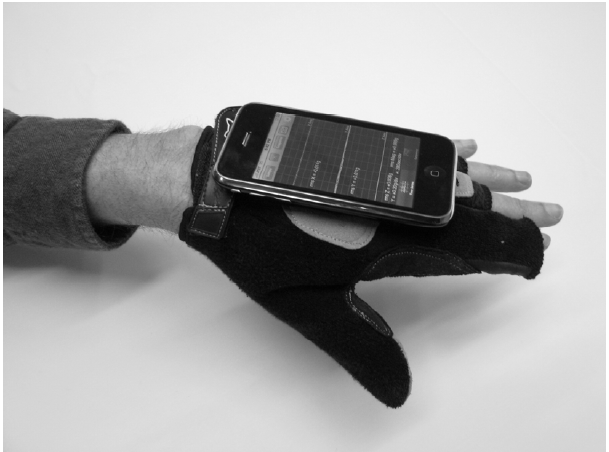
\includegraphics[scale=0.3]{./img/moyne-iphone.png}
  % matrixargseg.png: 296x162 pixel, 100dpi, 7.52x4.11 cm, bb=0 0 213 117
  %\caption{Estágio desenvolvimento de jogos ~\cite{fullerton2008game}}
\caption[Aplicação para \textit{smartphone} com a finalidade de identificar sinais de tremor]{Aplicação para iPhone com a finalidade de identificar sinais de tremor ~\cite{lemoyne2010}}
 %  \caption{Estágio desenvolvimento de jogos}
 \label{fig:iphone-tremor}
\end{figure}


Como apresentado nos trabalhos relacionados, as soluções existentes para~\ac{sms} dos sinais motores utilizam sensores vestíveis (\textit{wearables}), que comumente são incorporados à roupa ou ao corpo do usuário~\cite{classifiersparkinson2014}. De acordo com a perspectiva do usuário, estes sensores são considerados invasivos e estereotipados~\cite{aarhus_negotiating_2010}. Por outro lado, o gerenciamento medicamentoso do~\ac{dp} necessita de um cuidado acurado e diário~\cite{parkself2015,quantitativeparkinson2011}. Por este motivo, é que esta tese pretende prover um mecanismo para quantificar os sinais motores do~\ac{dp} através da indução da execução dos movimentos.


\section{Objetivos}\label{section:objetivos}
Nesta tese, tem-se como objetivo a conceber uma solução computacional que induza o usuário a executar movimentos para avaliação motora. Pretende-se usar jogos eletrônicos como forma de: \textbf{induzir}, \textbf{motivar} e abstrair o monitoramento de dados de saúde de uma maneira \textbf{não invasiva} e longe do \textbf{contexto de tratamento de saúde}.

Nesta tese, foi proposto uma arquitetura de software para o desenvolvimento de jogos eletrônicos integrados a um SMS, onde, demonstrou-se a viabilidade desta arquitetura com a implementação de um jogo capaz de monitorar um sintoma do~\ac{dp}, como estudo de caso.

%Objetivou-se criar um~\ac{sms} integrado à um jogo eletrônico capaz de: induzir a execução de uma avaliação motora que torne possível o processamento dos sinais biomecânicos e consequentemente identificar a presença de sintomas do~\ac{dp}. 

A avaliação da tese foi realizada em duas etapas: na primeira, avaliou-se a capacidade de monitoramento dos indivíduos com \ac{dp} em um estudo analítico de caso-controle; na segunda, avaliou-se a possibilidade de inserir este monitoramento na rotina diária dos pacientes. O estudo analítico de caso-controle, onde foi realizado uma avaliação com 30 sujeitos de pesquisa (15 do grupo controle e 15 diagnosticados com~\ac{dp}). Como resultado, foi identificado e quantificado o sintoma da bradicinesia. Para distinguir os grupos (caso-controle e diagnosticados com~\ac{dp}), utilizamos uma~\ac{svm} para classificação dos dados~\cite{datamining2005}, com a qual obteve-se uma acurácia de 86,66\%. Avaliou-se a adequação da abordagem de monitoramento dos sinais motores na rotina diária usando jogos eletrônicos, aplicando a técnica~\ac{gqm}~\cite{van1999goal}. Nesta avaliação, 90,00\% dos avaliados consideraram a abordagem não-invasiva e incorporável a rotina diária. 

\section{Metodologia}
Esta pesquisa foi submetida à avaliação pelo Comitê de Ética da UFCG (\textbf{CAAE: 14408213.9.1001.5182})~\footnote{Plataforma Brasil, url: http://aplicacao.saude.gov.br/plataformabrasil/} (Apêndice~\ref{sec:comite}), somente depois da aprovação deste é que os dados foram coletados. A metodologia de pesquisa possui aspectos qualitativos e quantitativos. Referente ao aspecto qualitativo, buscou-se identificar a importância desta tese junto à comunidade de especialistas da área de saúde (Seção~\ref{sec:entrevista_semi_estruturada}). Nos aspectos quantitativos, essa pesquisa fez uma análise do sensores de movimento e avaliou a acurácia da aquisição de sinais motores e possibilidade de identificar os sinais do~\ac{dp} baseado na Cinemática Angular do Movimento Humano. Por meio dos dados coletados, pudemos classificar a normalidade e dificuldade na execução de movimentos de abdução e adução dos braços~\cite{mcginnis2013biomechanics}, como será apresentado na Seção~\ref{sec:resultado_svm}. Para avaliar a aceitabilidade da proposta sob a perspectiva do usuário, utilizou-se uma análise~\ac{gqm} a qual é uma abordagem hierárquica que inicia com objetivo principal e o divide em questões mensuráveis~\cite{saraiva2006}, como será apresentado na Seção~\ref{gqm_usuarios}.

Em resumo, três questões foram utilizadas como base para a definição da metodologia do trabalho em três diferentes etapas sequenciais:
	\begin{description}
	\item[QUESTÃO 1] Quais os benefícios de acompanhar os sinais motores do paciente diariamente, do ponto de vista do profissional da saúde?
	\item[QUESTÃO 2] Como melhor adquirir e quantificar sinais motores utilizando sensores de movimento para monitorar os sinais de \ac{dp}?
	\item[QUESTÃO 3] Na perspectiva dos usuários, a abordagem de quantificar os sinais motores é considerada não-invasiva e aplicável à rotina diária?
	\end{description}

As seguintes atividades foram realizadas para a execução do trabalho:

\begin{enumerate}

\item{Realizar revisão bibliográfica e coleta de requisitos junto a profissionais de saúde.}

\item{Definir o conceito da abordagem, denominada \ac{jogue-me}, baseada em captura de sinais motores através de sensores de movimento, utilizando jogos eletrônicos e processamento dos sinais para transformá-los em informações de saúde.}


\item{Analisar a perspectiva dos profissionais de saúde em relação ao acompanhamento dos sinais motores dos pacientes com~\ac{dp} (os profissionais foram indagados sobre a melhora na tomada de decisão quanto ao acompanhamento dos sinais) e verificar se os parâmetros motores, como velocidade angular e amplitude do movimento dos braços, são importantes para realizar o acompanhamento dos sinais do~\ac{dp}. Procurou-se encontrar, junto ao profissional de saúde, a importância do monitoramento dos sinais motores e os benefícios trazidos por este, através de uma abordagem de pesquisa qualitativa. Com esta pesquisa, foi possível validar a \textbf{QUESTÃO 1}, que consiste em verificar a importância do acompanhamento de sinais motores integrados à rotina diária do paciente.}

\item{Validar o uso de sensores para classificação dos dados através do processamento dos sinais motores adquiridos por sensores de movimento utilizados em jogos eletrônicos. A classificação consistiu em aplicar os sinais numa~\ac{svm} para distinguir indivíduos do grupo controle ante indivíduos diagnosticados com~\ac{dp}.
O resultado dessa pesquisa demonstrou a viabilidade da abordagem e, consequentemente, validou a \textbf{QUESTÃO 2} do trabalho.}

\item{Definir a arquitetura de software que viabilizou tecnicamente a abordagem~\ac{jogue-me}. Nesta pesquisa, definimos um arcabouço de software para encapsular o desenvolvimento de jogos com essa abordagem.}

\item{Validar a solução~\ac{jogue-me} do ponto de vista computacional. A solução foi validada através da implementação da arquitetura e do desenvolvimento de jogos. Com esta etapa, demonstrou-se ser possível realizar monitoramento de dados motores de forma não invasiva, ou seja, sem os jogadores perceberem que estão fornecendo dados de saúde.}

\item{Verificar junto ao público alvo (portadores de~\ac{dp}) os requisitos de usabilidade, adequação à rotina diária, segurança física e se a proposta é considerada invasiva na perspectiva do paciente. Com esta avaliação, avaliou-se a \textbf{QUESTÃO 3} da pesquisa.}

\end{enumerate}

\subsection{Termo de Consentimento Livre e Esclarecido (TCLE)}
Antes da realização da coleta dos dados, expomos aos sujeitos da pesquisa as informações necessárias para a realização do estudo. Desta maneira, o indivíduo consentiu com sua participação através da assinatura do Termo de Consentimento Livre e Esclarecido~\footnote{Resolução Nº 196/96, do Conselho Nacional de Saúde, do Ministério da Saúde (CNS/MS).} (Apêndice~\ref{sec:comite}). 

\subsection{Relação Risco Benefício da Pesquisa}
Os riscos inerentes podem decorrer da exposição de dados dos participantes da pesquisa, o que pode acarretar danos morais e/ou psicológicos. Por esse motivo, foram tomados todos os cuidados para que a identidade do indivíduo não fosse revelada, garantindo assim, privacidade e confidência das informações. Todos os dados coletados, estão disponibilizados para pesquisa futura, permitindo o uso para pesquisa a todas instituições envolvidas (UFCG, UFAL e IFAL). No entanto, preservamos a identidade dos participantes da pesquisa e omitimos todos os dados que permitissem sua identificação, conforme descrito no Termo de Consentimento Livre e Esclarecido.

Durante a realização da pesquisa com os participantes da pesquisa, houve uma preocupação referente a possíveis constrangimentos por parte do sujeito da pesquisa. Caso, não conseguisse realizar a pesquisa ou responder alguma pergunta devido ao comprometimento da doença. O pesquisador prestou total assistência, orientando-os adequadamente. Mas, salienta-se que os riscos apresentados justificam-se pelo benefício de monitorar os sinais do~\ac{dp} para um melhor tratamento da doença.


\subsection{Confidencialidade}
Os dados do estudo em questão são considerados propriedade conjunta das partes envolvidas (UFCG, UFAL e IFAL). Porém, sua utilização por terceiros necessita de prévia autorização de todos. No entanto, na submissão do Projeto ao Comitê de Ética da UFCG (\textbf{CAAE: 14408213.9.1001.5182}), expressou-se o comprometimento em tornar público os resultados da pesquisa, sejam estes favoráveis ou não.


\section{Contribuições}
Nas últimas décadas, o monitoramento e quantificação dos sinais motores têm sido objeto de pesquisa recorrente na computação, eletrônica, bioinformática e saúde~\cite{reviewassesenspark2015}. As pesquisas nessa áreas, são fundamentais para a compreensão do progresso de doenças crônicas como o~\ac{dp} e também para auxiliar os médicos no acompanhamento de seus pacientes.

Nesta tese, foi desenvolvida uma arquitetura de software (Capítulo~\ref{arquitetura_captura}) que permite: quantificar, avaliar e identificar o sintoma de bradicinesia do~\ac{dp} induzindo o usuário a executar movimentos de avaliação motora, de uma forma lúdica e integrada a um jogo eletrônico, e longe do contexto de tratamento da saúde.

Do ponto de vista clínico, tornou-se possível identificar como está a saúde do paciente e em que momento o tratamento medicamentoso é eficaz. Atualmente, um detalhamento das flutuações motoras do~\ac{dp} é realizado por auto-relatórios em avaliações diárias dos pacientes que informam em que período do dia a medicação está surtindo efeito~\cite{reviewassesenspark2015}. No entanto, para uma avaliação dos sintomas motores mais acurado, é necessário poder induzir a execução de movimentos para avaliação motora de modo a mensurar quantitativamente os sintomas do~\ac{dp}~\cite{wiiassesspark2016}.

Por estes argumentos apresentados, foi desenvolvido nesta tese um mecanismo quantitativo de avaliação da eficácia do tratamento que utiliza um jogo eletrônico que induz o usuário a executar movimentos de avaliação motora de uma maneira não-invasiva. Esta abordagem de monitoramento, resulta em benefícios aos médicos para um tratamento mais efetivo e acurado da dosagem medicamentosa. Os resultados obtidos, com arquitetura de software desenvolvida, permitiu identificar e estimar a gravidade do sintoma da bradicinesia e das complicações motoras mensuradas num estudo de caso-controle, e isto é um resultado bastante relevante para esta tese.

Como possível cenário de uso da pesquisa, supondo que um paciente de uma doença crônica como o~\ac{dp} faz uso de medicamento antiparkinsoniano e possui um jogo de monitoramento de sinais do~\ac{dp} em sua residência, caso ele utilize o jogo em diferentes momentos do dia, os sinais podem ser quantificados sem a presença de um profissional de saúde, que poderia visualizar a melhora ou piora do estado de saúde do seu paciente ao longo dos dias. A partir da presente abordagem, o médico, ao possuir a informação, poderia gerenciar melhor a dosagem medicamentosa e, consequentemente, prolongar a qualidade de vida do paciente~\cite{abn2010}.

%
%Atualmente, os jogos são aplicados para melhora da saúde em diferentes contextos. No entanto, nenhum dos trabalhos relacionados pretendem identificar sinais para monitorar o estado de saúde. Logo, este trabalho visa desenvolver um ambiente de jogo que motive a execução de movimentos específicos, com o propósito de quantificar os sinais motores dos usuários.
%
%No entanto, alinhar a jogabilidade e a capacidade de monitoramento dos sinais de saúde não é trivial, pois deve ser levado em consideração o uso dos sensores e deve-se definir quais movimentos ou ações permitem a identificação dos sinais motores. Por este motivo, a proposta de um~\ac{sms} dos sinais motores usando jogos necessita de um acompanhamento de um profissional de saúde para supervisionar e auxiliar nas definições dos movimentos e ações dos usuários. 

%Posteriormente, na posse dessas ações, deverá ser testada a execução dessas atividades e sua aquisição para uma possível classificação dos dados conforme proposto nesta tese.
%os trabalhos já existentes~\cite{Ballegaard:2008:HEL:1357054.1357336,patel_monitoring_2009,visionbased2009,bachlin_parkinsons_2009,albanese2012}.
%De posse dos movimentos e da captura dos dados será feito um levantamento de um \textit{game design} que permita executar os movimentos em  um ambiente lúdico e divertido como um jogo para entretenimento ~\cite{sweetser2005-gameflow}.



\section{Organização do Documento}
O restante deste documento está organizado da seguinte forma:
\begin{itemize}
	\item No Capítulo~\ref{chapter:fundamentacao} está descrita a fundamentação teórica relacionada ao trabalho.
	\item No Capítulo~\ref{chapter:abordagem_gahme} está definida a abordagem \ac{jogue-me} para indução e monitoramento dos sinais motores de maneira não invasiva usando jogos eletrônicos.
	\item No Capítulo~\ref{chapter:arquitetura_captura} é apresentada a arquitetura de software da abordagem.
	\item No Capítulo~\ref{chap:avaliacao} são apresentados os experimentos realizados para avaliar a tese.
	\item No Capítulo~\ref{chapter:conclusoes_futuros} são apresentadas as conclusões do trabalho e propostos trabalhos futuros.
\end{itemize}

\chapter{Fundamentação Teórica}\label{chapter:fundamentacao}
Neste capítulo, pretende-se oferecer ao leitor uma visão geral das principais áreas nas quais esse trabalho está fundamentado. Mais especificamente, apresenta-se uma explanação sobre o~\ac{dp}, seus sinais motores, os estágios da doença, o uso da cinemetria como ferramenta para medição dos parâmetros cinemáticos do movimento humano, e a~\ac{svm} como classificador de dados para a identificação dos padrões presentes em um conjunto de dados.


\section{Doença de Parkinson}\label{section:doenca_parkinson}
O termo Parkinsonismo é genérico e designa uma série de doenças com causas diferentes, que têm em comum a presença de sinais frequentemente encontrados no~\ac{dp}. Esta doença é uma das muitas formas de parkinsonismo, correspondendo a cerca de 75$\%$ dos casos. Os sinais associados ao~\ac{dp}~\cite{protpar010} são causados pela degeneração dos neurônios dopaminérgicos presentes na substância negra. O~\ac{dp} é mais comum em idosos, porém existem casos precoces de início da doença em indivíduos antes dos 40 anos ou até mesmo abaixo dos 21~\cite{menezes2003}. A incidência da doença é estimada de 100 a 200 casos por 100.000 habitantes e, com o avanço da idade populacional, o contingente de pessoas diagnosticadas com ~\ac{dp} tende a aumentar.

O~\ac{dp} é uma doença progressiva e incapacitante e, após os 10 anos de tratamento, o custo operacional, o impacto social e financeiro aumentam vertiginosamente. Estima-se que o custo anual mundial com medicamentos antiparkinsonianos esteja em torno de 11 bilhões de dólares, tornando-se de 3 a 4 vezes mais caro nas fases avançadas da doença~\cite{protpar010}. Outro fator crucial para a escolha do~\ac{dp} como objeto de estudo é a variação dos sinais motores ao longo do dia em virtude da resposta ao tratamento medicamentoso. Portanto, a abordagem de monitorar os sinais, em diferentes momentos do dia, permite um melhor gerenciamento da doença e, como consequência, uma melhora na qualidade de vida dessa população.


%TODO verificar a regencia do verbo acarretar: se for indireto mantém o em; caso contrário remove-o
Atualmente, o levodopa é o tratamento medicamentoso mais utilizado para o tratamento de redução dos sinais do~\ac{dp}. Porém, sua efetividade é reduzida ao longo do tempo, o que requer um aumento progressivo das dosagens ou o uso de outros tratamentos associados. Isso acarreta em um gerenciamento complexo entre drogas e seus respectivos efeitos colaterais. Portanto, ao buscar prolongar a qualidade de vida dos pacientes com o uso deste tratamento, é recomendável um gerenciamento medicamentoso com uma dosagem mínima~\cite{national2006parkinson}, para reduzir os sinais motores e prolongar a qualidade de vida do paciente. Como o gerenciamento medicamentoso é de responsabilidade do neurologista, este o faz de acordo com as visitas clínicas dos pacientes, quando estes ou seus cuidadores fazem relatos sobre o progresso do tratamento. Contudo, esta avaliação clínica é realizada de forma esporádica e subjetiva~\cite{protpar010,quantitativeparkinson2011}. Dessa maneira, é necessária uma quantificação destes sinais 
para um tratamento mais adequado e preciso. 

Com o surgimento do tratamento para o \ac{dp} é possível manter uma mobilidade funcional durante anos, além de aumentar a expectativa de vida dos pacientes tratados~\cite{abn2010}. Os fármacos do grupo dos antiparkinsonianos, como a levodopa, permitem restaurar a atividade dopaminérgica que se encontra reduzida; dessa maneira, as drogas aliviam os sinais característicos da doença. Entretanto, devido aos efeitos colaterais frequentes induzidos pelos fármacos, é preciso iniciar o tratamento com esses medicamentos somente quando os sinais estiverem prejudicando o desempenho profissional ou as atividades diárias do paciente~\cite{abn2010}. A natureza progressiva do~\ac{dp} e suas manifestações clínicas (motoras e não motoras) estão associadas a efeitos colaterais precoces e tardios da intervenção terapêutica, o que torna o tratamento da doença bastante complexo~\cite{protpar010}. Estima-se que a taxa de morte dos neurônios dopaminérgicos da substância negra situa-se ao redor de 10$\%$ ao ano~\cite{national2006parkinson}. Consequentemente, com o passar do tempo, a sintomatologia parkinsoniana tende a evoluir, o que aumenta a necessidade de uma maior dosagem medicamentosa, pois a resposta aos medicamentos decresce com o progresso da doença~\cite{protpar010}.

 
\subsection{Diagnóstico}
Os sinais mais característicos do~\ac{dp} e que são frequentemente usados para diagnosticar a doença são~\cite{rowlandtratado}: tremor em repouso (que diminui durante movimentos voluntários); bradicinesia (lentidão e escassez de movimentos, além de dificuldade na marcha); rigidez muscular (aumento da resistência ao movimento passivo dos membros); e perda de reflexos posturais, que leva à alteração da marcha e aumenta a ocorrência de queda~\cite{abn2010,tolosa06}. 

A evolução da doença, a gravidade e a progressão dos sinais variam de um paciente para outro. Atualmente, não existe teste diagnóstico estabelecido para a doença, e os estudos comprovam dificuldade na diferenciação clínica entre o~\ac{dp} e outras formas de parkinsonismo. A maioria dos neurologistas concorda que o diagnóstico do~\ac{dp} requer a identificação de alguma combinação de sinais motores cardinais, como: tremor de repouso, bradicinesia, rigidez tipo roda denteada e alterações posturais. No entanto, uma classificação clínica padrão ainda não foi obtida~\cite{protpar010}. Além do mais, um diagnóstico auxiliar importante é a resposta dos pacientes aos medicamentos antiparkinsonianos, tal como a levodopa~\cite{protpar010}. Os protocolos clínicos~\cite{protpar010,national2006parkinson} sugerem que o diagnóstico do~\ac{dp} está diretamente relacionado à resposta satisfatória ao levodopa. No entanto, uma resposta satisfatória à levodopa não confirma o diagnóstico do~\ac{dp}~\cite{rowlandtratado}, porque 
existem muitos casos de parkinsonismo sintomáticos e muitas formas de síndromes de Parkinson, que, em seus estágios iniciais, respondem bem ao levodopa. 

Atualmente, os critérios estabelecidos pelo Banco de Cérebros da Sociedade de Parkinson do Reino Unido~\cite{national2006parkinson} são os mais utilizados para diagnosticar a doença (Apêndice \ref{apendice:diagnostico_parkinson}). 







\subsection{Principais Sinais do Parkinson}
Nesta seção serão descritos sintomas motores mais frequentes do~\ac{dp}~\cite{protpar010} e que foram objetos deste estudo.

\subsubsection{Tremor}\label{sec:tremor}
O tremor é o sintoma mais frequente e mais perceptível~\cite{jankovic2008} do~\ac{dp}, embora não seja o mais incapacitante. No entanto, para a maioria dos pacientes, este sinal é o principal motivo que os leva a procurar ajuda médica. Sua principal característica é o rítmico relativamente lento quando comparado a outros tipos de tremor (4 a 7 ciclos por segundo), em que sua maior frequência é quando o membro está em repouso, sendo denominado de tremor de repouso. No início da enfermidade, o tremor ocorre em um lado (tremor assimétrico), e assim permanece por diferentes períodos de tempo. Situações de estresse emocional ou a sensação de ser observado aumentam, visivelmente, a intensidade do tremor~\cite{jankovic2008}. 

Por ser um sinal relacionado ao repouso do membro, os usuários cessavam o sinal assim que eram confrontados com um jogo eletrônico desenvolvido para quantificação do tremor. Por esse motivo, não foi possível desenvolver um jogo que quantificasse este sinal.


\subsubsection{Bradicinesia}\label{section:analise_bradicinesia}
Enquanto que o sintoma de tremor é o mais visível do~\ac{dp}, a bradicinesia é o sintoma mais incapacitante da doença. A bradicinesia consiste numa lentidão do movimento voluntário e num comprometimento de todos os movimentos associados a ele. A acinesia é uma progressão da bradicinesia e implica na ausência completa do movimento voluntário, sem a perda da força muscular~\cite{do2007parkinson}.

A bradicinesia pode estar presente nos sinais iniciais do~\ac{dp}, em diferentes partes do corpo: olhos, com a redução do movimento de piscar; face, com a redução das expressões faciais; voz robótica, devido à redução da velocidade dos músculos das cordas vocais; e redução do movimento dos membros superiores e inferiores~\cite{do2007parkinson}. Normalmente, nos estágios iniciais da doença, a bradicinesia é acompanhada de: rigidez dos músculos, assimetria dos movimentos entre os membros e dificuldade nos movimentos (por exemplo, levantar de uma cadeira, virar na cama ou andar).  

\subsection{Escalas e os Estágios da Doença}\label{section:escalas_avaliacao}
A partir dos tratamentos do~\ac{dp}, foram criadas escalas de avaliação do progresso da doença~\cite{updrs87,goul05}. Essas escalas permitem avaliar a condição clínica geral, incapacidades, funções motoras, mentais e até mesmo a qualidade de vida dos pacientes. Esses instrumentos são importantes tanto no nível clínico quanto no científico, pois permitem monitorar a progressão da doença e a eficácia do tratamento medicamentoso~\cite{updrs87,goul05}.  Por conseguinte, foi criada em 1987 a Escala Unificada de Avaliação da  Doença de Parkinson (\textit{Unified Parkinson’s Disease Rating Scale – UPDRS})~\cite{updrs87}, que é amplamente utilizada para monitorar o progresso da doença e a eficácia do tratamento. Segundo Goulart~\cite{goul05}, as escalas de estágios de incapacidade representadas por \textit{Hoehn/Yahr} e a \textit{UPDRS}~\cite{updrs87} são consideradas as de maior confiabilidade, podendo ser usadas por fisioterapeutas para melhor avaliação do estado clínico-
funcional do  paciente.% 


Segundo a \textit{UPDRS}, a evolução do~\ac{dp} é classificada nas seguintes fases ~\cite{updrs87}:
  \begin{itemize}
    \item \textbf{ESTÁGIO 0:} Nenhum sinal da doença;
    \item \textbf{ESTÁGIO 1:} Doença unilateral;
    \item \textbf{ESTÁGIO 1,5:} Envolvimento unilateral e axial;
    \item \textbf{ESTÁGIO 2:} Doença bilateral sem déficit de equilíbrio;
    \item \textbf{ESTÁGIO 2,5:} Doença bilateral leve, com recuperação no “teste do empurrão”;
    \item \textbf{ESTÁGIO 3:} Doença bilateral leve a moderada; alguma instabilidade postural; capacidade para viver independente;
    \item \textbf{ESTÁGIO 4:} Incapacidade grave, ainda capaz de caminhar ou permanecer de pé sem ajuda;
    \item \textbf{ESTÁGIO 5:} Confinado à cama ou à cadeira de rodas.
  \end{itemize}

A \textit{UPDRS} é composta por 42 itens, divididos em quatro partes: atividade mental; comportamento e humor; atividades de vida diária; exploração motora e complicações da terapia medicamentosa. Estes itens, são avaliados por autorelato ou observação clínica. Dessa maneira subjetiva, é realizada a classificação do estágio da doença no paciente. Contudo, justamente por ser baseada em autorelato e observação clínica, a qual é realizada eventualmente com a presença de um profissional, pesquisadores questionam a efetividade da análise do estágio da doença e propõem alternativas para avaliação dos itens motores de forma quantitativa, através de sensores, os quais permitem quantificar os sinais motores do paciente~\cite{kostek12,synnott_wiipd_2012,patel_monitoring_2009}. Os sinais bradicinéticos são avaliados por intermédio da parte motora da tabela de avaliação UPDRS~\cite{updrs87}, através de exercícios como tocar as pontas dos dedos, pronar e supinar o antebraço.

A identificação dos sinais do~\ac{dp} durante a rotina diária permite um diagnóstico mais precoce da doença e, consequentemente, a obtenção de benefícios para um tratamento mais duradouro. Além disso, o monitoramento dos efeitos da medicação junto ao paciente permite um melhor gerenciamento medicamentoso e, assim, uma redução dos efeitos colaterais do tratamento e um prolongamento da sua qualidade de vida~\cite{rowlandtratado}.


\section{Cinemetria}
A \textbf{Cinemetria} consiste em um conjunto de métodos para medição dos parâmetros cinemáticos do movimento humano, tais como: posição, orientação, velocidade e aceleração~\cite{mcginnis2013biomechanics}. Os instrumentos básicos das medidas cinemáticas podem ser adquiridos por câmeras de vídeo; pela análise das imagens e dos movimentos; e  por meio de software específico, os quais calculam as variáveis cinemáticas de interesse. Atualmente, com o uso de câmeras infravermelho, é possível reconhecer o movimento humano e calcular as grandezas cinemáticas das características do movimento com precisão e robustez~\cite{gabel2012}.

A cinemetria relaciona técnicas e métodos para o processamento de grandezas cinemáticas; entre elas, destacam-se as técnicas de medição direta~\cite{mcginnis2013biomechanics}, utilizadas para: 
\begin{enumerate}
	\item medidas de tempo;
	\item medidas de ângulos;
	\item medidas de amplitude;
	\item medidas de velocidade angular.
\end{enumerate}

\subsection{Movimento Angular}
O movimento angular ocorre quando todas as partes do corpo se movem pelo mesmo ângulo, mas não realizam o mesmo deslocamento linear. A subdivisão da cinemática que trata do movimento angular é chamada de cinemática angular, que permite examinar o movimento angular a partir de segmentos de um movimento, divididos em partes identificáveis que aumentam a compreensão do movimento humano~\cite{hamill1999bases}. 

Quase todos os movimentos humanos envolvem as rotações de segmentos do corpo. Os segmentos giram sobre os centros articulares que formam os eixos de rotação para esses segmentos~\cite{hamill1999bases}. No movimento angular, a unidade de medida utilizada é o grau(º) e a unidade de tempo é o segundo(s). Logo, as velocidades angulares calculadas são mensuradas em °/s.

A anatomia funcional consiste no estudo dos componentes do corpo, necessários para desempenhar um movimento ou uma função humana, como, por exemplo, a abdução ou a adução do braço (Figura \ref{fig:movabducaoaducao}).

\begin{figure}
 \centering
 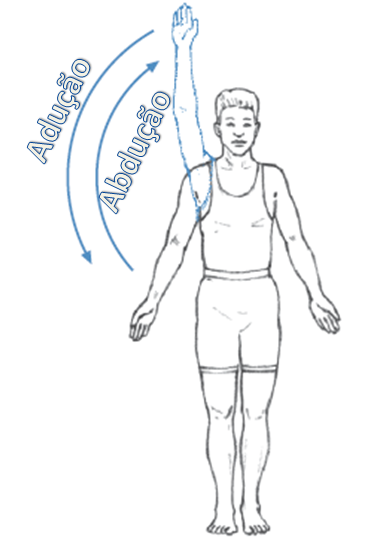
\includegraphics[scale=0.5]{./img/abducao.png}
 % matrixargseg.png: 296x162 pixel, 100dpi, 7.52x4.11 cm, bb=0 0 213 117
 %\caption{Estágio desenvolvimento de jogos ~\cite{fullerton2008game}}
\caption[Movimentos de abdução e adução do braço]{\copyright Movimentos de Abdução e Adução do Braço~\cite{mcginnis2013biomechanics}}
%  \caption{Estágio desenvolvimento de jogos}
 \label{fig:movabducaoaducao}
\end{figure}

Na análise biomecânica do movimento humano, são calculados dois tipos de ângulos:
	\begin{itemize}
		\item Ângulo Relativo: este ângulo é formado entre os eixos longitudinais de segmentos corporais adjacentes~\cite{hamill1999bases}. Logo, os ângulos relativos não descrevem a posição de segmentos ou os lados do ângulo no espaço. Se um indivíduo tem um ângulo relativo de 90º no cotovelo e esse ângulo é mantido, o braço pode ficar em qualquer posição. A interpretação dada a cada segmento irá determinar o tipo de movimento realizado. 
		\item Ângulo Absoluto: este ângulo identifica a orientação angular de um segmento corporal em relação a uma linha fixa de referência~\cite{hamill1999bases}. Dessa forma, os ângulos absolutos devem ser medidos na mesma direção a partir de uma única referência, seja ela horizontal ou vertical.
	\end{itemize}

\section{Máquina de Vetor de Suporte (SVM)}\label{sec:svm_linear}
A teoria da aprendizagem estatística fornece um conjunto de técnicas para a análise de dados, a qual permite a aquisição de conhecimento~\cite{vapnik95}. A máquinas~\ac{svm} faz uso de um conjunto de métodos de aprendizagem supervisionada~\cite{datamining2005} para classificação de dados. Ou seja, a~\ac{svm} é uma ferramenta de predição de classificação, que usa a teoria da aprendizagem de máquina e busca maximizar a acurácia. Normalmente, a~\ac{svm} é aplicada para classificação binária, ou seja, permite classificar os dados em duas classes. No entanto, essa técnica também tem sido aplicada em dados com mais de duas classes~\cite{multisvm2011}.

Optou-se por utilizar a~\ac{svm} devido a sua capacidade de generalização nos problemas de classificação de dados~\cite{vapnik95,xusvm2009}, sua robustez nos resultados~\cite{xusvm2009} e sua performance com baixa complexidade computacional em comparação a outras abordagens como redes neurais~\cite{comprnasvm2007}.


%O uso de Máqui-nas de Vetores de Suporte, no entanto, apresentou-se como sendo mais econômico computacionalmente, atingindo a taxa limite do sistema de aquisição de vídeo, 29.97 quadros por segundo em um classifica-dor contínuo do alfabeto manual da Linguagem Bra-sileira dos Sinais. O sistema de classificação baseado em SVM implementado neste trabalho, mostra-se um classifi-cador mais rápido que RNAs de baixa complexidade computacional, atingindo taxas de reconhecimento similares.
%
%~\cite{comprnasvm2007}

%
%O uso de uma rede neural de baixa complexida-de computacional permite uma considerável redução do tempo de processamento do sistema, atingindo taxas de 28.1 quadros por segundo. 
%

%The connection of robustness and regularization in the SVM context is important for the following reasons. First, it gives an alternative and potentially powerful explanation of the generalization ability of the regularization term. In the standard machine learning view, the regularization term bounds the complexity of the class of classifiers. The robust view of regularization regards the testing samples as a perturbed copy of the training samples. Therefore, when the total perturbation is given or bounded, the regularization term bounds the gap between the classification errors of the SVM on these two sets of samples. In contrast to the standard PAC approach, this bound depends neither on how rich the class of candidate classifiers is, nor on an assumption that all samples are picked in an i.i.d. manner.~\cite{xusvm2009}


%This work considers the relationship between robust and regularized SVM classification. In particular, we prove that the standard norm-regularized SVM classifier is in fact the solution to a robust classification setup, and thus known results about regularized classifiers extend to robust classifiers. To the best of our knowledge, this is the first explicit such link between regularization and robustness in pattern classification. The interpretation of this link is that norm-based regularization essentially builds in a robustness to sample noise whose probability level sets are symmetric unit balls with respect to the dual of the regularizing norm. It would be interesting to understand the performance gains possible when the noise does not have such characteristics, and the robust setup is used in place of regularization with appropriately defined uncertainty set~\cite{xusvm2009}

%Based on the robustness interpretation of the regularization term, we re-proved the consistency of SVMs without direct appeal to notions of metric entropy, VC-dimension, or stability. Our proof suggests that the ability to handle disturbance is crucial for an algorithm to achieve good generalization ability. In particular, for “smooth” feature mappings, the robustness to disturbance in the observation space is guaranteed and hence SVMs achieve consistency. On the other-hand, certain “non-smooth” feature mappings fail to be consistent simply because for such kernels the robustness in the feature-space (guaranteed by the regularization process) does not imply robustness in the observation space.~\cite{xusvm2009}

Um classificador~\ac{svm} foi inicialmente desenvolvido para problemas de aprendizagem linearmente separáveis e utiliza vetores de separação, através de uma técnica de hiperplano de separação ótima\cite{vapnik95}. O hiperplano tenta separar as diferentes classes, maximizando a margem entre os pontos extremos de cada classe~\cite{valt2010}. O melhor hiperplano de uma~\ac{svm} é aquele que possui a maior margem entre as duas classes, como pode ser visto na Figura ~\ref{fig:hiperplano}.  

\begin{figure}
 \centering
 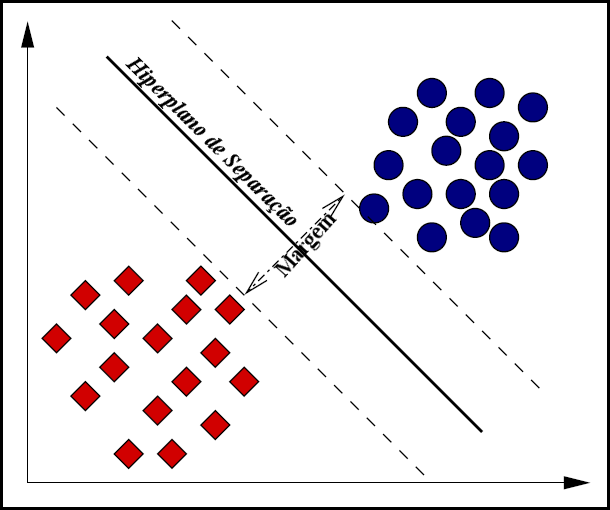
\includegraphics[scale=0.4]{./img/svmhyperplane.png}
 % matrixargseg.png: 296x162 pixel, 100dpi, 7.52x4.11 cm, bb=0 0 213 117
 %\caption{Estágio desenvolvimento de jogos ~\cite{fullerton2008game}}
\caption{Hiperplano de separação para duas classes}
%  \caption{Estágio desenvolvimento de jogos}
 \label{fig:hiperplano}
\end{figure}


Para entender o funcionamento da ~\ac{svm}, é necessário conhecer a notação:
\begin{math}
R^{n}
\end{math}
é um número real n-dimensional no espaço de vetores. Onde os pontos \textbf{u}, \textbf{v}, \textbf{w} e \textbf{x} serão utilizados para denotar pontos em 
\begin{math}
R^{n}
\end{math}.
Estes pontos são chamados de vetores ou padrões na literatura de Aprendizagem de Máquina.

Cada ponto possui $x_{i}$ e um rótulo $y_{i}$, que denotam a qual classe $x_{i}$ pertence. Logo, se $y_{i} = + 1$, então $x_{i}$ pertence a classe 1; e caso $y_{i} = - 1$, então $x_{i}$ pertence a classe 2. A classificação binária como o nome sugere, significa classificar os dados em duas classes. Para tanto, primeiramente os dados do grupo de treinamento são usados para preencher os espaços com pontos. E depois um segundo grupo de teste é aplicado para verificar a hipótese de qual classe aquele ponto pertence. Formalmente, dado um conjunto de pontos $x_{i}$, qual será os valores $y_{i}$ correspondentes, dado que o classificador possui os padrões adquiridos do grupo de treinamento, além dos rótulos associados a sua classe. A~\ac{svm} irá usar o hiperplano de separação para tentar dividir os dados de treinamento em duas classes. Dessa maneira, o resultado da classificação dos dados de teste dependerá da localização da projeção desses dados.

Formalmente, classificadores que separam os dados por meio de um hiperplano utilizam um discriminante~\cite{valt2010} de Equação~\ref{eq:hiperplano}. Um hiperplano é considerado de Margem Máxima (ou de Separação Ótima) quando uma função discriminante consegue separar um conjunto de vetores sem erro. Uma função é discriminante quando consegue discriminar os valores em diferentes padrões. 

O produto escalar $ w.x $ entre os vetores $ w $ e $ x $, $ w $ é o vetor normal ao hiperplano descrito, o vetor \textbf{w} é denominado de peso e a constante parâmetro \textbf{b} é chamada de \textit{bias} ou desvio.
\linebreak
\begin{equation}
f(x)=w^Tx+b=0
\label{eq:hiperplano}
\end{equation}

Se \textbf{u} e \textbf{v} são dois padrões e \textit{f(x)} é a função discriminante, então os valores de \textit{f(\textbf{u})} e \textit{f(\textbf{v})} irão auxiliar na determinação dos valores de \textbf{u} e \textbf{v} que pertencem a classe; logo, a regra para a predição da classe está no Código~\ref{codepredicaoclasse}. 

\begin{lstlisting}[frame=single, caption=Código de Predição da Classes, label=codepredicaoclasse]  % Start your code-block

classificacao = 0;
if (w^t.x + b > = 0)
	classificacao = 1
else
	classificacao = -1;
endif
\end{lstlisting}

A partir desse método de separação dos dados, é que a~\ac{svm} foi aplicada para classificar indivíduos diagnosticados com~\ac{dp} ante indivíduos sem o diagnóstico estabelecido. Para corroborar com a nossa escolha de SVM, encontrou-se trabalhos de classificação de indivíduos com parkinson utilizando a mesma abordagem~\cite{bradmonitor2015,svmparkinson2010,patel_monitoring_2009}. No entanto, o que diferencia este trabalho dos demais, é que os dados classificados foram adquiridos utilizando a abordagem de um jogo eletrônico que induz o paciente a executar movimentos para a avaliação motora~\cite{quantitativeparkinson2011,wiiassesspark2016}. 


\section{Conclusão}
Neste capítulo, foi explicitado os motivos para quantificar os comprometimentos motores do~\ac{dp}. Para avaliar a saúde motora, foi utilizado os estudos cinemáticos do movimento humano para quantificar as amplitudes do movimento e a velocidade angular dos mesmos. 

A identificação do sintoma foi realizada por meio da máquina de aprendizagem, SVM, aqui descrita. A SVM recebe como dados de entrada os valores dos parâmetros motores e identifica-o como saudável ou parkinsoniano.

Nos capítulos seguintes, serão apresentados o Processador de Dados Biomecânicos (Seção~\ref{sec:processador_bio}) responsável por extrair as características do movimento~\cite{mcginnis2013biomechanics} para obter o resultado da classificação da SVM exposta na Seção~\ref{sec:resultado_svm}.

%
%pretende-se oferecer ao leitor uma visão geral das principais áreas nas quais esse trabalho está fundamentado. Mais especificamente, apresenta-se uma explanação sobre o~\ac{dp}, seus sinais motores, os estágios da doença, o uso da cinemetria como ferramenta para medição dos parâmetros cinemáticos do movimento humano, e a~\ac{svm} como classificador de dados para a identificação dos padrões presentes em um conjunto de dados.
%
%Neste capítulo, estão descritas
 %%será explicado como são extraídos os pontos, usando os vetores de características
%%Por este motivo, será apresentado 


\chapter{Abordagem~\textit{JOGUE-ME}}\label{chapter:abordagem_gahme}
Para desenvolver um~\ac{sms} dos sinais motores, usando jogos eletrônicos como interface de entrada de dados, é necessário analisar que movimentos e ações o usuário deve executar para que seja possível identificar os sinais motores, a partir de suas ações. Estes movimentos devem ser testados junto a indivíduos portadores da deficiência a ser monitorada e indivíduos como grupo de controle para avaliar a viabilidade de detecção do sinal.

\section{Definição dos Requisitos da Abordagem}\label{section:requisitos_solucao}
Com base no levantamento bibliográfico e nas entrevistas semiestruturadas~\cite{FLI04} com profissionais de saúde, identificamos e enumeramos os seguintes requisitos funcionais, os quais devem ser desenvolvidos para uma solução~\ac{jogue-me}:



\begin{description}
	\item[REQ-JOGUE-ME-01 - Pontuação e Taxa de Acerto:] O jogador percebe os objetivos e visualiza o sucesso ou o fracasso alcançado. O jogo pontua o jogador de acordo com seus erros e acertos~\cite{Suhonen:2008:SFE:1457199.1457204,sinclair07}.
	\item[REQ-JOGUE-ME-02 - Progresso e Evolução do Jogador e dos Desafios:] O jogador percebe seu progresso e sua evolução no jogo. Os desafios tonam-se mais complexos no decorrer do tempo ~\cite{Suhonen:2008:SFE:1457199.1457204}.
	\item[REQ-JOGUE-ME-03 - Estado de Fluxo]: Um dos grandes desafios de um jogo eletrônico é levar o usuário a um ``Estado de Fluxo'' ou escapismo, passando a executar a atividade proposta pelo jogo de uma forma autotélica, ou seja, o usuário não vislumbra um benefício imediato ou futuro ~\cite{sweetser2005-gameflow}. 
	\item[REQ-JOGUE-ME-04 - Preocupação com Integridade Física do Jogador:] Promover atividades físicas ou ações que venham a trazer injúria ao jogador, como: movimentos de equilíbrio, movimentos repetitivos ou bruscos~\cite{arntzen2011,sinclair07}.
	\item[REQ-JOGUE-ME-05 - Aquisição e Armazenamento de Sinais Motores:] O jogo deve realizar a aquisição dos sinais motores do usuário usando sensores de movimento. Os dados capturados são enviados a um servidor para tornar possível o acompanhamento da saúde motora.
	\item[REQ-JOGUE-ME-06 - Mecanismo de Identificação de Sinais Motores:] Baseados em algoritmos de aprendizagem de máquina, o servidor acompanha todos os usuários do sistema e identifica qual deles está com distúrbio motor; em caso afirmativo, envia-se a informação ao profissional de saúde.
	\item[REQ-JOGUE-ME-07 - Mecanismo de Visualização dos Parâmetros Motores do Usuário:] O profissional de saúde poderá visualizar os dados identificados pela máquina de aprendizagem, para realizar a tomada de decisão sobre o estado de saúde do usuário.
\end{description}



\section{Visão geral da solução}
%Colocar aqui para testar um melhor posicionamento
\begin{figure}[h]
     \centering
     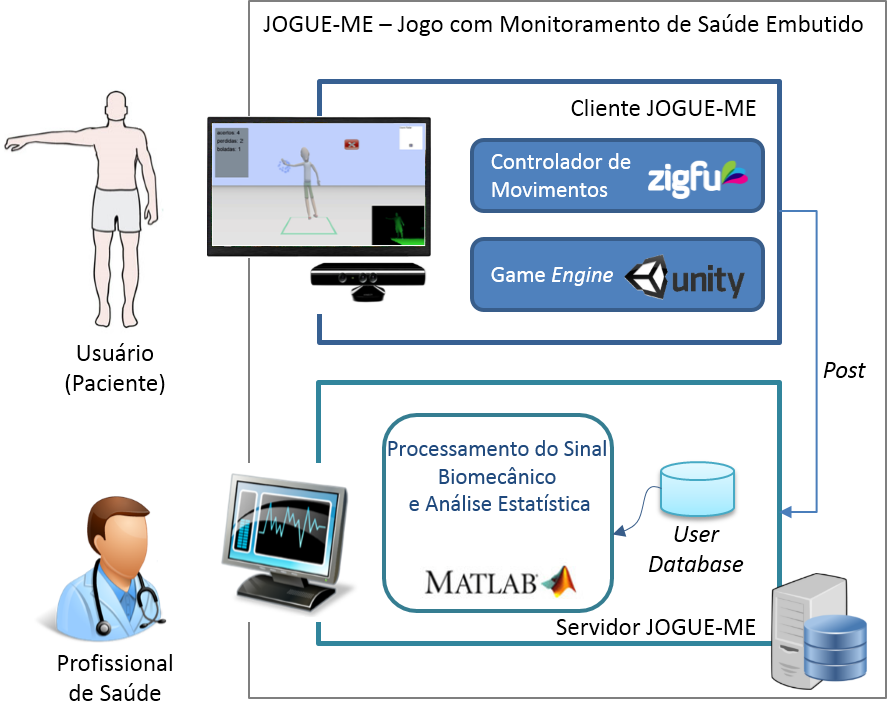
\includegraphics[width=0.78\textwidth]{./img/visaosistema.png}
     \caption{Visão geral da abordagem~\textit{JOGUE-ME}}
     \label{img:visaogeral}
\end{figure}
A abordagem~\ac{jogue-me} faz uso de jogos eletrônicos como interface de aquisição de sinais, tornando os usuários mais motivados a fornecer seus sinais motores, em comparação ao uso dos dispositivos vestíveis~\cite{alemdar}. Então, com o uso da presente abordagem, um paciente portador de uma doença motora, no conforto do seu lar, poderá fornecer sinais motores de uma maneira colaborativa e não invasiva. Por outro lado, o profissional de saúde poderá visualizar os sinais motores de seus pacientes com uma frequência muito maior, em comparação às avaliações clínicas realizadas durante o período de consulta. 

Nesse estudo, ao utilizar jogos eletrônicos como mecanismo para entrada de dados, é possível alcançar os requisitos de não invasividade identificados nesta tese, pois, através dos dispositivos de sensores de movimento usados nesses ambientes, é possível desenvolver um jogo que motive o usuário a executar ações específicas para permitir o monitoramento de sinais motores. A partir de uma interface com o usuário, que permite enviar os dados capturados a um servidor, e armazenar estes dados para o acompanhamento da saúde motora por parte do profissional de saúde.

Para esta solução, propõe-se usar técnicas de processamento de sinais para reconhecer os padrões de movimento e identificar os sinais motores (Figura~\ref{img:visaogeral}). Para tornar isso factível é necessário identificar ciclos de movimento, filtrá-los e extrair características deste movimento. Após a extração das características, os dados são repassados para máquinas de aprendizagem, as quais são responsáveis por classificar os dados, baseadas em evidências estatísticas. Caso a máquina identifique algum usuário com distúrbio motor, ela poderá notificar o profissional de saúde para que este visualize os dados e tenha um melhor suporte para a tomada de decisão em relação ao tratamento.

O funcionamento da abordagem pode ser descrito como uma composição de quatro passos: aquisição dos sinais por meio de sensores, processamento de sinais biomecânicos, classificação dos dados e visualização. Estes passos são detalhados nas seções seguintes.

\section{Aquisição dos Sinais Por Meio de Sensores}
O cliente \ac{jogue-me} é um jogo com funcionalidades de aquisição de dados motores de movimentos específicos. Logo, ele realiza a captura e o envio de dados para um servidor, que recebe requisições para efetuar o recebimento e o armazenamento das informações, o que torna possível armazenar o histórico do usuário para um acompanhamento dos sinais motores por um longo período. Com o uso do~\ac{jogue-me} é possível adquirir os movimentos do paciente para identificar a evolução dos sinais do~\ac{dp}, e consequentemente, quantificar sua saúde motora. 

Atualmente, a análise dos sintomas motores é feita de forma subjetiva pelo cuidador ou esporádica pelo neurologista quando o paciente está em atendimento clínico, visto que, atualmente não existem mecanismos disponíveis em larga escala que permitam quantificar os sintomas motores ou acompanhar o tratamento a distância. Este projeto pretende atender a esta demanda e auxiliar a prática dos profissionais de saúde melhorando a qualidade de vida dos pacientes com~\ac{dp}.

Um sensor de movimentos como o MS-Kinect~\cite{kinnect2013}, por exemplo, possui uma câmera infravermelho capaz de reconhecer os movimentos de todo o corpo humano e identificar as posições das articulações anatômicas~\cite{hamill1999bases}, para análise da cinemática do movimento humano~\cite{mcginnis2013biomechanics}. 

Para mensurar os movimentos do paciente, utilizamos diretrizes médicas para avaliação motora do~\ac{dp} como a UPDRS~\cite{updrs87}, a qual, permite diagnosticar e acompanhar o progresso da doença. Logo, os dados adquiridos pelos sensores podem ser mensurados com o processamento dos sinais e reconhecimento de padrões para identificar a ocorrência de sintomas motores. 

Desta maneira, a aquisição dos sinais motores e a quantificação do movimento de seus usuários permitirá uma participação mais precisa do profissional de saúde.



\section{Processamento de Dados Biomecânicos}\label{sec:processador_bio}
%Estou colocando aqui para ver uma melhor posição
\begin{figure}[!htb]
     \centering
     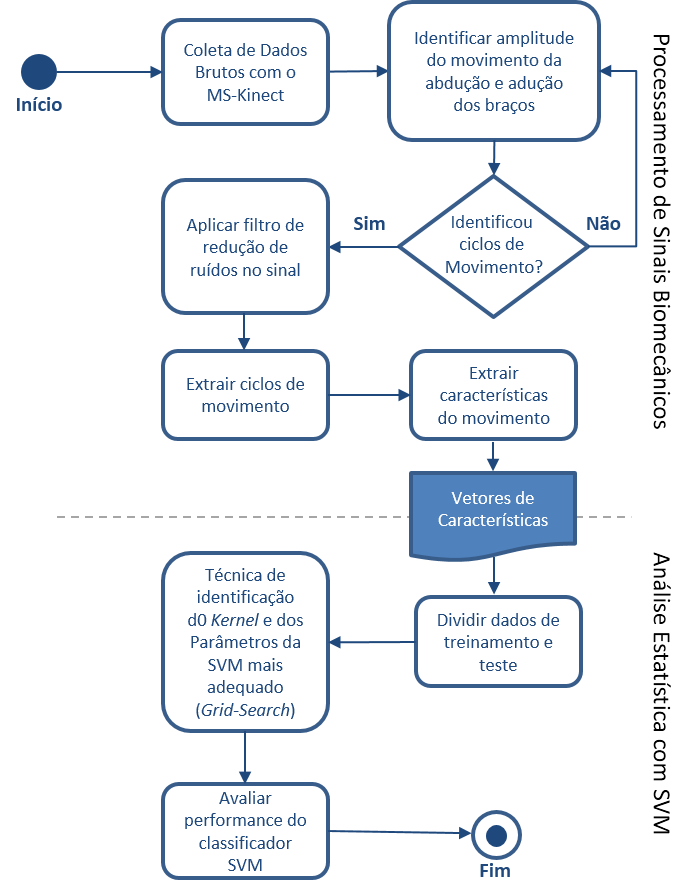
\includegraphics[width=0.8\textwidth]{./img/biomecprocessor2.png}
     \caption{Processamento de sinais biomecânicos.}
     \label{img:process_bio}
\end{figure}
O módulo de Processamento de Dados Biomecânicos é responsável por filtrar, remover ruídos e identificar ciclos de movimento para uma posterior extração dos vetores de características, como pode ser visto na Figura~\ref{img:process_bio}. A partir dos sinais processados, aplicam-se técnicas de aprendizagem de máquina para obter a classificação dos sinais e, consequentemente, validar este trabalho.




\subsection{Identificação de Ciclos de Movimento}\label{section:identificao_ciclos}

Os sinais adquiridos por sensores de movimento possuem bastante ruído, o que dificulta a identificação dos ciclos de movimento, pois eles possuem uma posição que inicia o ciclo de movimento, como na Figura~\ref{img:exsinalposicaopunho}, e o ruído existente pode cruzar por essa linha e consequentemente gerar falsas identificações. 

\begin{figure}[!htb]
     \centering
     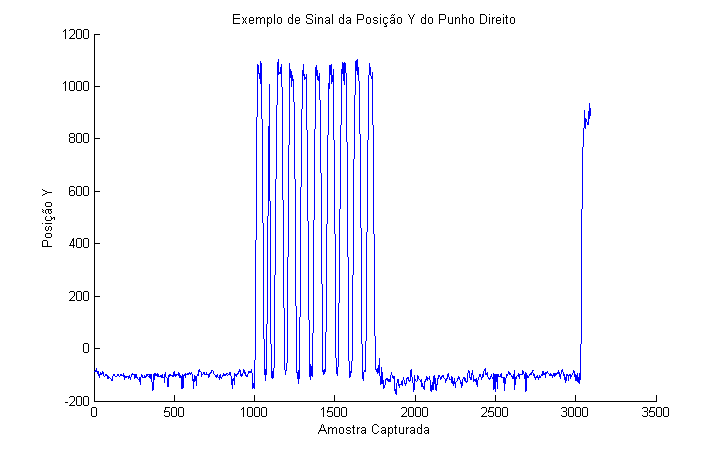
\includegraphics[width=1\textwidth]{./img/exsinalposicaoypunhodireito.png}
     \caption{Exemplo de sinal capturado da articulação do punho direito usando MS-Kinnect na posição Y}
     \label{img:exsinalposicaopunho}
\end{figure}


Em casos de análise de sinais biomecânicos da amplitude do movimento, é possível aplicar a técnica de detecção de picos e vales do sinal~\cite{peakdetect}. Esta técnica consiste em usar um valor de referência, $\delta$\ (\textit{delta}), para identificação dos picos, e descartar valores menores que são considerados ruídos. O pico é o ponto mais alto entre os 2 pontos mais baixos, que são considerados os vales do ciclo. A técnica é aplicada no sinal, com um $\delta$\ de 500, obtendo-se como resultado os picos e os vales identificados como pode ser visto na Figura~\ref{img:expicosvales}.

\begin{figure}[!htb]
     \centering
     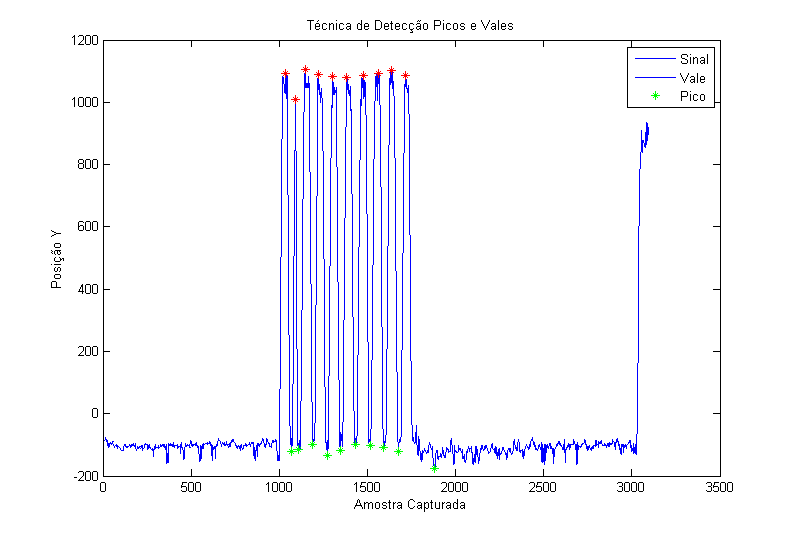
\includegraphics[width=1\textwidth]{./img/deteccaopicosvales.png}
     \caption{Exemplo da aplicação da técnica de detecção de picos e vales no sinal}
     \label{img:expicosvales}
\end{figure}


%\subsubsection{Redução de Ruídos no Sinal}
O processo de Identificação de Ciclos de Movimento é realizado em 3 etapas distintas:
\begin{itemize}
	\item identificar ciclos de movimentos;
	\item calcular movimento angular realizado durante o ciclo de movimento;
	\item remover ciclos de movimentos incompletos.
\end{itemize}

Para identificar os ciclos de movimento de adução e abdução dos braços, é necessário utilizar uma das articulações como referência. Neste movimento, a articulação do punho (Figura~\ref{img:exsinalposicaopunho}) é a que possui o sinal com maior amplitude entre as demais; por esse motivo, esta é a escolhida para identificar os ciclos. Realiza-se a técnica de picos e vales no sinal do \textit{punho} para identificar o início e o fim do movimento de adução e abdução dos braços. Depois de identificado onde começa e termina o movimento, calcula-se o deslocamento angular através do produto escalar entre as articulações do punho, do ombro e da bacia (Seção~\ref{section:movimento_abducao}). Neste momento, o sinal irá conter ciclos de movimentos angulares, então realiza-se uma nova eliminação de ruídos, ao extrair os ciclos de movimento identificados no sinal. Essa é a primeira etapa da filtragem dos dados, a qual seleciona o início e o fim dos ciclos de movimentos. Depois desta etapa, realiza-se a extração de cada ciclo e identifica-se sua completude, para que as características extraídas dos ciclos de movimento sejam semelhantes para cada indivíduo e torne possível a classificação dos dados.


%\begin{figure}[!htb]
     %\centering
     %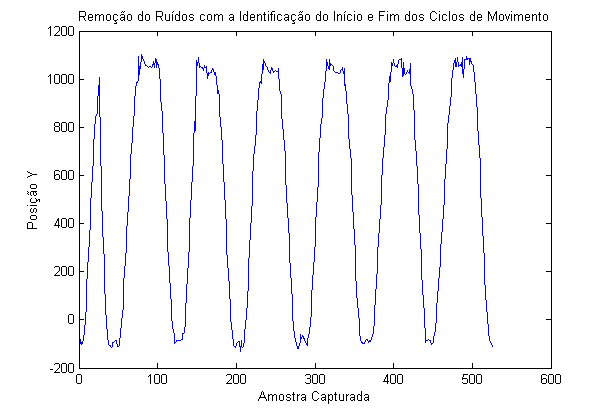
\includegraphics[width=1\textwidth]{./img/remocaoruidociclo.png}
     %\caption{Remoção de Ruídos}
     %\label{img:remocaoruidossinal}
%\end{figure}


\subsection{Extração das Características do Movimento} \label{sec:extracao_caracteristcas}
As características do sinal a ser obtido são baseadas na cinemática do movimento angular. Logo, é necessário um estudo da biomecânica do movimento humano nos ciclos de movimento~\cite{hamill1999bases}. De posse do tempo de ocorrência de cada ciclo e das articulações do \textbf{punho}, da \textbf{bacia} e do \textbf{ombro}, deve-se calcular o ângulo relativo do movimento de abdução e adução do braço através da aplicação do teorema do produto escalar, que encontra o ângulo entre dois vetores dentro do intervalo de $0 \leq \theta \leq 180º$.

\subsubsection{Cálculo do Ângulo Relativo do Movimento de Abdução e Adução}\label{section:movimento_abducao}
O produto escalar é uma operação entre dois vetores cujo resultado é um escalar~\cite{algebra2000}. Então, o ângulo entre dois vetores é definido como ``o menor'' ângulo entre eles. Dessa forma, este ângulo está dentro do intervalo de $0 \leq \theta \leq 180º $. O produto escalar é o ângulo de $ \theta$ formado entre os vetores $ v $ e $ w $.


% \begin{equation}
% cos(\theta) = (v . w) /  (||v|| ||w||) 
% \label{eq:produto_escalar}
% \end{equation}
% 
% 
% \begin{figure}[!htb]c
%      \centering
%      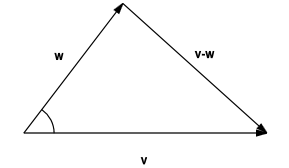
\includegraphics[width=0.5\textwidth]{./img/produtoescalar.png}
%      \caption{Produto Escalar Entre 2 Vetores}
%      \label{img:produto_escalar}
% \end{figure}

No movimento de abdução e adução do braço, o ângulo relativo pode ser calculado com as posições ($ x $\ ,  $ y $\ , $ z $\ ) das articulações (\textit{quadril}, \textit{ombro} e \textit{punho}). Utilizando o produto escalar entre esses pontos, extraem-se as características do movimento, como amplitude do movimento, e, quando relacionamos com o tempo, conseguimos extrair a velocidade angular deste movimento, como pode ser visto na Figura~\ref{img:amplitude_braco}, quantificando o movimento da adução e abdução do braço em relação ao tempo.


\begin{figure}[!htb]
     \centering
     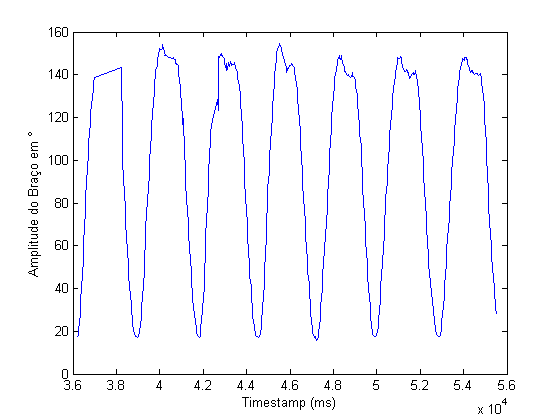
\includegraphics[width=1\textwidth]{./img/amplitude-braco.png}
     \caption{Amplitude do movimento de abdução e adução}
     \label{img:amplitude_braco}
\end{figure}

\subsubsection{Cálculo da Velocidade Angular do Movimento de Abdução e Adução}
O pico da amplitude do movimento irá conter a amplitude máxima desse movimento. O tempo gasto entre o 1° vale e o pico em cada ciclo de movimento, será o tempo gasto para a abdução do braço, e o tempo gasto entre o pico e o 2° vale de cada ciclo, será o tempo gasto para a adução do braço. Portanto, com a amplitude máxima e o tempo gasto nesses movimentos, podem ser calculadas as velocidades angulares de abdução e adução dos braços, como pode ser visto na Figura~\ref{img:amplitude_braco_picos_vales}.
\begin{figure}[!htb]
     \centering
     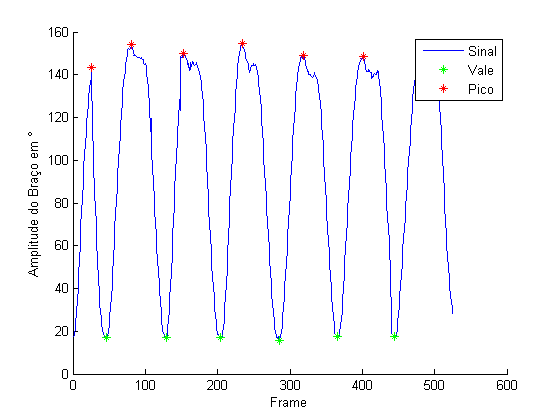
\includegraphics[width=1\textwidth]{./img/amplitude-braco-picos.png}
     \caption{Detecção de picos e vales na amplitude do movimento de abdução e adução do braço}
     \label{img:amplitude_braco_picos_vales}
\end{figure}

\subsection{Filtragem de Dados}\label{section:filtro_dados}

A filtragem dos dados consiste na realização das seguintes etapas nos ciclos de movimento:
\begin{description}
	\item [Escalonamento dos ciclos]: O conjunto de dados deve possuir a distribuição de \textbf{M} amostras de vetores de dimensão \textbf{n}. Como os dados a serem analisados são sinais, deve-se então escalonar o sinal para uma dimensão \textbf{n} para poder realizar o cálculo matricial quadrático de (\textbf{M} x \textbf{n}).		
	\item [Normalização dos ciclos]: Em estatística, o termo normalização possui diferentes significados ~\cite{statisticterms2006}. Neste trabalho, a normalização consiste no ajuste dos valores dos dados em torno do valor máximo. Ou seja, o máximo valor obtido dos dados terá o valor 1, e os demais serão obtidos a partir da divisão do valor máximo. A normalização se faz necessária para que a variação dos dados seja mantida, além de facilitar a identificação de similaridades~\cite{vicini2005}. 	
	\item [Cálculo do Vetor Médio dos Ciclos]: Para definir a completude de um ciclo de movimento, deve-se calcular a média entre todos os ciclos de movimento, que é o vetor médio dos ciclos escalonados e normalizados. O \textbf{vetor médio}, Equação (\ref{eq:vetormedio}), chamado de $\bar{X}$, consiste na média aritmética de todos os ciclos de movimento, ou seja, ele define a centralização dos dados ~\cite{statisticshandbook2009}. 	
		\begin{equation}
			\bar{X}=\frac{\sum_{i=1}^{n}(Xi)}{(n)}
			\label{eq:vetormedio}
		\end{equation}
	\item [Calculo da Variância de Cada Ciclo ao Vetor Médio]: A variância é uma medida de dispersão estatística, que indica o quão longe os dados estão de um valor esperado~\cite{statisticshandbook2009}. Neste caso, o valor esperado é o vetor médio dos ciclos ($\bar{X}$), e a variância, Equação (~\ref{eq:variancia}), irá nos informar o quão distante cada ciclo ($C$) está em relação a média.
		\begin{equation}
			var(C) = (C - \bar{X} )^2
			\label{eq:variancia}
		\end{equation}
		
		
	\item [Definição do limiar para remoção de ciclos]: Essa etapa do processo de filtragem não é trivial, pois deve-se definir uma constante, $ filtro $\, que será comparada à variância do ciclo. Se esta for menor, será aceita; caso contrário, removida. Contudo, balancear entre o limiar de dispersão do ciclo de movimento e a média é complexo, pois existe uma grande variabilidade de movimento. Logo, um limiar muito alto pode acarretar na remoção de uma grande quantidade de ciclos. Por outro lado, um limiar baixo colocaria ruídos nos dados e, consequentemente, impactaria no resultado da classificação.	
	%\lstset{language=Matlab}
	%\begin{lstlisting}[frame=single, caption=Filtro dos Ciclos]  % Start your code-block
		%
    %filtro = 1;
    %vetorMedio = mean(ciclos);
    %varianciaCiclo = sum(ciclo - (vetorMedio).^2);
    %remocao = varianciaCiclo>filtro;
	%\end{lstlisting}
	%
\end{description}

	%\begin{figure}
     %\centering
     %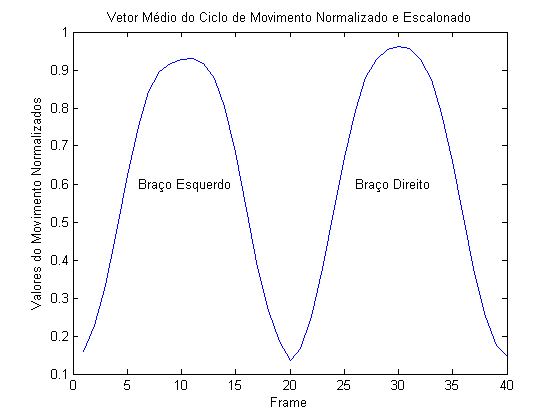
\includegraphics[width=1\textwidth]{./img/vetormedionormalozadoescalonado.png}
     %\caption{Ciclos de Movimento Normalizados e Escalonados}
		 %\label{img:ciclos_normalizado_escalonado}
	%\end{figure}

Como exemplo, temos um ciclo de movimento removido (Figura~\ref{img:ciclo_filtrado}), com \textit{valor do filtro = 1} e o \textit{valor da variância = 2,3078}.

\begin{figure}[!htb]
     \centering
     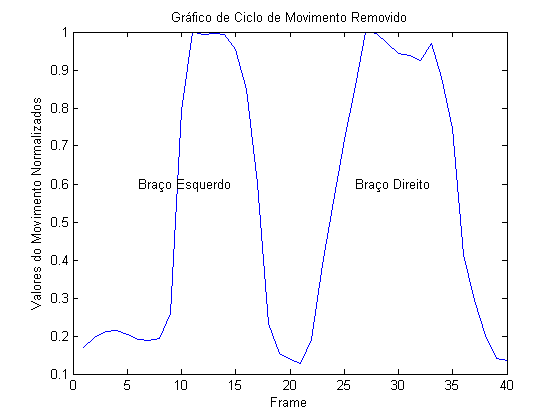
\includegraphics[width=1\textwidth]{./img/ciclomovimentoremovido.png}
     \caption{Ciclo de movimento removido}
		 \label{img:ciclo_filtrado}
\end{figure}


\section{Classificação de Dados por Máquina de Aprendizagem}\label{section:class_dados}
O objetivo de todo esse processo de identificação de ciclos, extração de características e filtragem é justamente facilitar a separação dos dados por máquinas de aprendizagem. A normalização dos ciclos ficou como o resultado do cálculo do produto escalar, que nos retorna valores entre $ 0° $\ a $ 180° $\, do movimento de abdução e adução. O escalonamento de cada ciclo de movimento ficou com 20 \textit{frames}. Como temos o movimento do braço esquerdo e depois o do direito, temos um total de 40 \textit{frames} por ciclo. O motivo pelo qual decidimos juntar os ciclos dos braços esquerdo e direito foi justamente para facilitar a identificação da assimetria do movimento existente nos estágios iniciais do~\ac{dp}. Portanto, o classificador será responsável por identificar os indivíduos diagnosticados com~\ac{dp}, por meio das diferenças de movimento existente entre estes e os indivíduos sem o diagnóstico da doença. 

O vetor de características é composto dos ciclos de movimento e das características extraídas de cada ciclo, conforme explicado na Seção~\ref{sec:extracao_caracteristcas}. Ou seja, terá, além do ciclo de movimento, os valores da velocidade angular de abdução e adução do braço esquerdo e direito. De posse desse vetor de características e do rótulo sobre a classe do ciclo de movimento (indivíduo diagnosticado com~\ac{dp} e indivíduo sem o diagnóstico estabelecido), esses dados serão repassados como entrada-saída para o classificador de dados, que irá dividir entre grupos de treinamento e teste para realizar sua classificação.

Nesta abordagem, o classificador de dados será usado para identificar usuários com problemas motores. Dessa forma, irá auxiliar o profissional de saúde no acompanhamento de seus pacientes. Supondo que um profissional de saúde detém um grande número de pacientes, e que estes fazem uso da abordagem~\ac{jogue-me} para monitorar seus dados, caso fosse identificada alguma anormalidade motora, o profissional de saúde seria notificado e poderia visualizar as informações que poderiam auxiliar na tomada de decisão.





\section{Visualização dos Dados}
O acompanhamento dos sinais motores é necessário, principalmente, para doenças crônicas de impacto motor e que tenham melhoria nos sinais, pois dessa maneira auxilia o médico no acompanhamento motor e, consequentemente, permite tratar o paciente de acordo com a resposta ao tratamento.

Como exemplo da abordagem, o profissional de saúde poderia visualizar as características dos movimentos, que serviram como dados de entrada para a máquina de aprendizagem. Nesse caso, podemos ver duas tabelas em que é possível identificar as diferenças motoras de uma pessoa diagnosticada com ~\ac{dp} (Tabela~\ref{table:extracao-caracteristica}) e um indivíduo sem o diagnóstico da doença (Tabela~\ref{table:extracao_caracterisca_saudavel}).

\begin{table}[h]
\begin{tabular}{|r|r|r|r|r|r|}
\hline
\multicolumn{4}{|l}{Velocidades º/S}                                                                                                                                                                                                                                                                                         & \multicolumn{2}{|l|}{Amplitudes}     \\ \hline
\multicolumn{1}{|l}{\textbf{\begin{tabular}[c]{@{}c@{}}Abdução\\ Esquerda\end{tabular}}} & \multicolumn{1}{|l|}{\textbf{\begin{tabular}[c]{@{}c@{}}Abdução\\ Direita\end{tabular}}} & \textbf{\begin{tabular}[c]{@{}c@{}}Adução\\ Esquerda\end{tabular}} & \textbf{\begin{tabular}[c]{@{}c@{}}Adução\\ Direita\end{tabular}} & \textbf{Esquerda} & \textbf{Direita} \\ \hline
78,95                                                                                    & 77,82                                                                                    & 83,06                                                              & 106,42                                                            & 130,00            & 124,72           \\ \hline
79,94                                                                                    & 34,68                                                                                    & 104,69                                                             & 39,98                                                             & 131,50            & 132,44           \\ \hline
81,05                                                                                    & 47,05                                                                                    & 107.38                                                             & 56,52                                                             & 132,22            & 123,66           \\ \hline
74,73                                                                                    & 47,09                                                                                    & 109,05                                                             & 47,75                                                             & 132,33            & 122,20           \\ \hline
72,01                                                                                    & 56,02                                                                                    & 102,36                                                             & 76,00                                                             & 131,40            & 119.75      \\ \hline
\end{tabular}
\caption{Extração das características do indivíduo com diagnóstico do Parkinson}
\label{table:extracao-caracteristica}
\end{table}

\begin{table}[h]
\begin{tabular}{|r|r|r|r|r|r|}
\hline
\multicolumn{4}{|l}{Velocidades º/S}                                                                                                                                                                                                                                                                                         & \multicolumn{2}{|l|}{Amplitudes}       \\ \hline
\multicolumn{1}{|l}{\textbf{\begin{tabular}[c]{@{}c@{}}Abdução\\ Esquerda\end{tabular}}} & \multicolumn{1}{|l|}{\textbf{\begin{tabular}[c]{@{}c@{}}Abdução\\ Direita\end{tabular}}} & \textbf{\begin{tabular}[c]{@{}c@{}}Adução\\ Esquerda\end{tabular}} & \textbf{\begin{tabular}[c]{@{}c@{}}Adução\\ Direita\end{tabular}} & \textbf{Esquerda} & \textbf{Amplitude} \\ \hline
129,35                                                                                   & 61,59                                                                                    & 78,74                                                              & 176,30                                                            & 159,39            & 143,50             \\ \hline
115,67                                                                                   & 118,15                                                                                   & 71,72                                                              & 79.46                                                             & 156,37            & 153,97             \\ \hline
120.96                                                                                   & 135,27                                                                                   & 66,70                                                              & 78,17                                                             & 154,30            & 149,91             \\ \hline
125.96                                                                                   & 137,43                                                                                   & 64,75                                                              & 81,57                                                             & 153,18            & 154,58             \\ \hline
139.99                                                                                   & 117,60                                                                                   & 69,96                                                              & 84,08                                                             & 151,68            & 148,90             \\ \hline
120,51                                                                                   & 111,92                                                                                   & 75,85                                                              & 75,18                                                             & 152,58            & 148,35             \\ \hline
\end{tabular}
\caption{Extração das características do indivíduo sem diagnóstico do Parkinson}
\label{table:extracao_caracterisca_saudavel}
\end{table}

Como pode ser visto nesses dados, a amplitude de um indivíduo diagnosticado com~\ac{dp} está bem menor do que em um indivíduo sem o diagnóstico estabelecido. Um valor importante também pode ser identificado na velocidade de adução esquerda do indivíduo com~\ac{dp}, pois este possui uma velocidade muito maior do que o indivíduo sem o diagnóstico. Possivelmente, porque um paciente com~\ac{dp} perde um pouco o controle sobre o membro, fazendo-o descer abruptamente~\cite{protpar010}. Dessa maneira, a abordagem pretende auxiliar o profissional de saúde com o fornecimento dessa informação, para que este efetue o acompanhamento e perceba a evolução do quadro clínico do paciente.

\section{Conclusão}
Neste capítulo, foram apresentados os requisitos que definiram a visão geral da abordagem~\ac{jogue-me}. Uma seção relevante deste capítulo é como será o processamento dos dados biomecânicos, nesta seção é demonstrada como será a extração de características a partir dos sinais adquiridos por sensores de movimento. Posteriormente, foi apresentada a importância da aprendizagem de máquina neste trabalho para identificar os usuários que possuem problemas motores.

Do ponto de vista clínico, foram citados os parâmetros cinemáticos quantificados que irá auxiliar o profissional de saúde na sua tomada de decisão. 

No capítulo seguinte, será apresentada a arquitetura de software que define a implementação da abordagem ~\ac{jogue-me}.
\chapter{Arquitetura de Software do~\textit{JOGUE-ME}}\label{chapter:arquitetura_captura}
Na concepção da arquitetura desenvolvida para implementar o~\ac{jogue-me} (Figura~\ref{fig:arquitetura}), foram definidos 3 elementos básicos: sensor de movimentos para adquirir os sinais motores e enviar ao cliente; cliente~\ac{jogue-me}, que é um jogo que interage com o usuário, induzindo a execução de movimentos para avaliação motora de uma maneira não-invasiva, e envia os dados a um serviço~\ac{jogue-me}; serviço~\ac{jogue-me}, que fica num estado de recebimento de dados e posterior repasse ao processador de dados biomecânicos, que processa e identifica a ocorrência dos sintomas motores por meio de uma máquina de aprendizagem.


%A arquitetura desenvolvida para implementar o~\ac{jogue-me} (Figura~\ref{fig:arquitetura}) descrita no Capítulo~\ref{chapter:abordagem_gahme}. 


%O objetivo desta arquitetura é que as atividades de desenvolvimento do jogo e identificação dos sintomas estejam separadas de acordo a suas responsabilidadesdelegar a responsabilidade de desenvolvimento do jogo à um desenvolvedor de jogos de modo que este, o desenvolvedor de jogos na abstração das dificuldades existentes no desenvolvimento de um jogo para monitoramento de dados da saúde motora. 

%Nesta tese foi desenvolvida uma arquitetura de software sob uma camada de software que é \textit{engine} de jogos bem difundida e utilizada (Unity 3D~\cite{unity3d}), que envia requisições de dados . Com a elaboração desta arquitetura de software busca-se facilitar a programação de jogos para o monitoramento da saúde motora ao criar Componentes de \textit{Software} que realizam este monitoramento. Assim ao usar esta arquitetura, descrita neste capítulo, os desenvolvedores de jogos podem criar \text{JOGUE-MEs} encapsulando os aspectos de processamento de sinal e reconhecimento da ocorrência dos sintomas motores. De acordo com a arquitetura 


%A arquitetura do sistema possui diferentes tecnologias, conforme definido na Figura. O objetivo principal para a definição desta arquitetura foi permitir que os jogos desenvolvidos utilizando esta abordagem desenvolvedor de jogos abstraia da e foi desenvolvida para permitir o desenvolvedor abstrair da complexidade do processamento do sinal dos dados e na identificação dos sintomas motores. 

%Logo, esta arquitetura de \textit{software} permite  integrada a uma \textit{engine} de jogos bem conhecida e difundida (Unity 3D~\cite{unity3d}) facilita o desenvolvimento de jogos para esse contexto.

%A arquitetura desenvolvida para o~\ac{jogue-me} busca abstrair das dificuldades existentes no desenvolvimento de um jogo para monitoramento de dados de saúde. Neste projeto foi desenvolvido um arcabouço de software, integrado a uma \textit{engine} de jogos bem difundida e utilizada por desenvolvedores de jogos. Devido a essa estrutura, buscamos facilitar a programação de jogos para a saúde, criando Componentes de \textit{Software} sobre a \textit{engine} de jogos Unity 3D~\cite{unity3d}. Assim, desenvolvedores de jogos podem criar \text{JOGUE-MEs}, usando esse arcabouço (Seção~\ref{sec:cliente_game}), o que permite ao desenvolvedor encapsular os aspectos de processamento de sinal. 


\begin{figure}[!h]
 \centering
  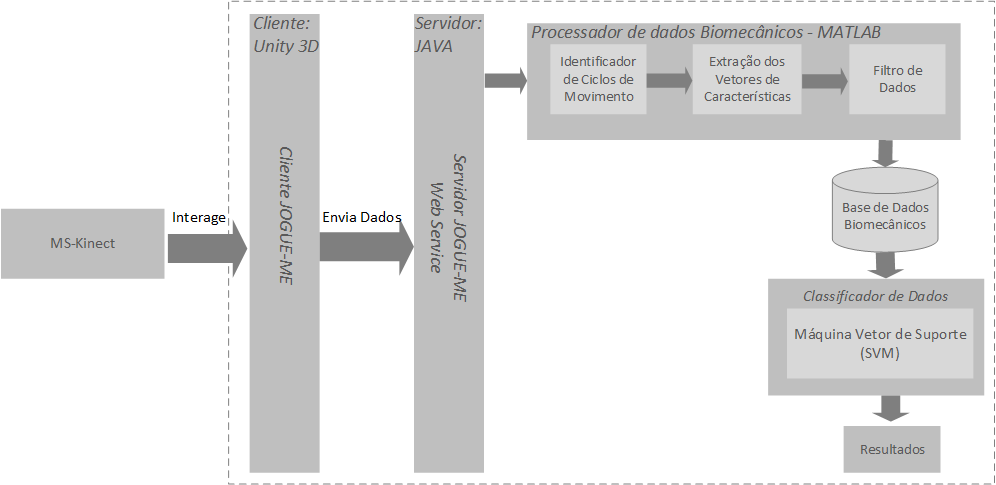
\includegraphics[scale=0.56]{./img/arquitetura.png}
 % matrixargseg.png: 296x162 pixel, 100dpi, 7.52x4.11 cm, bb=0 0 213 117
 %\caption{Estágio desenvolvimento de jogos ~\cite{fullerton2008game}}
\caption[Arquitetura de Software]{Arquitetura de Software}
%  \caption{Estágio desenvolvimento de jogos}
 \label{fig:arquitetura}
\end{figure}

\section{Arquitetura do ~\textit{JOGUE-ME}}\label{sec:cliente_game}
A arquitetura do~\ac{jogue-me} para o desenvolvimento de jogos utiliza uma \textit{engine} de jogos (Unity3D~\cite{unity3d}), que é um ambiente de desenvolvimento de jogos multi-plataforma. Esta \textit{engine} possibilita que os desenvolvedores abstraiam-se dos aspectos de hardware, plataforma e complexidade do desenvolvimento de jogos e habilita o desenvolvedor a se ater somente às atividades referentes ao desenvolvimento do jogo.

Atualmente, desenvolvedores independentes de jogos utilizam Unity3D~\cite{unity3d} como ferramenta de desenvolvimento. Esse ambiente facilita a criação de cenários, terrenos e interação com os objetos dos jogos usando uma linguagem de \textit{script}. No entanto, desenvolver jogos com propósito de monitorar sinais motores possui desafios que não precisam ser de responsabilidade dos desenvolvedores de jogos. Por esse motivo, criamos uma arquitetura de software para o cliente JOGUE-ME (Figura~\ref{fig:arquitetura_cliente}) que abstrai a complexidade do desenvolvimento de um jogo de monitoramento da saúde.

\begin{figure}[!htbp]
 \centering
 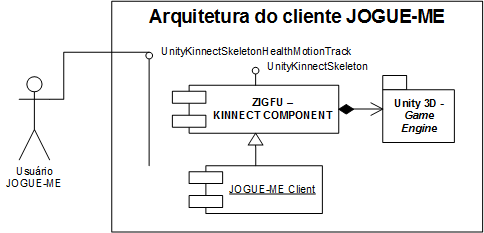
\includegraphics[scale=0.8]{./img/arquiclientejogueme.png}
 % matrixargseg.png: 296x162 pixel, 100dpi, 7.52x4.11 cm, bb=0 0 213 117
 %\caption{Estágio desenvolvimento de jogos ~\cite{fullerton2008game}}
\caption{Arquitetura JOGUE-ME: Módulo Cliente de Aquisição de Sinais Motores}
%  \caption{Estágio desenvolvimento de jogos}
 \label{fig:arquitetura_cliente}
\end{figure}


Para possibilitar a aquisição de sinais motores, este trabalho herdou do componente (Zigfu~\cite{zigfu}) para integrar o Ms-Kinnect~\cite{kinnect2013} como controlador do jogo à \textit{engine} de jogos Unity3D. O Ms-Kinnect~\cite{kinnect2013} é um sensor de captura de movimentos utilizado tanto para o console MS-XBOX 360 quanto para \textit{PCs}. Ele permite a aquisição dos sinais relativos ao movimento humano e identifica as articulações por meio da posição anatômica do corpo humano~\cite{hamill1999bases}.
%, como pode ser visto na Figura~\ref{fig:articulacoeskinnect}.



%Os jogos eletrônicos que fazem uso dos movimentos do corpo permitem a liberdade de movimento, logo o movimento exercido nestes possibilitam muita variabilidade. Logo, é necessário que o desenvolvedor tenha a informação de quais ações o jogador precisa executar para que estas sejam monitoráveis. As ações de um~\ac{jogue-me} devem estar descritas no~\ac{jogue-me}(Seção~\ref{subsec:game_actions_guide}) como estabelecido no processo de desenvolvimento proposto no Capítulo~\ref{chap:processo_desenvolvimento}.


%\begin{figure}[!htbp]
 %\centering
 %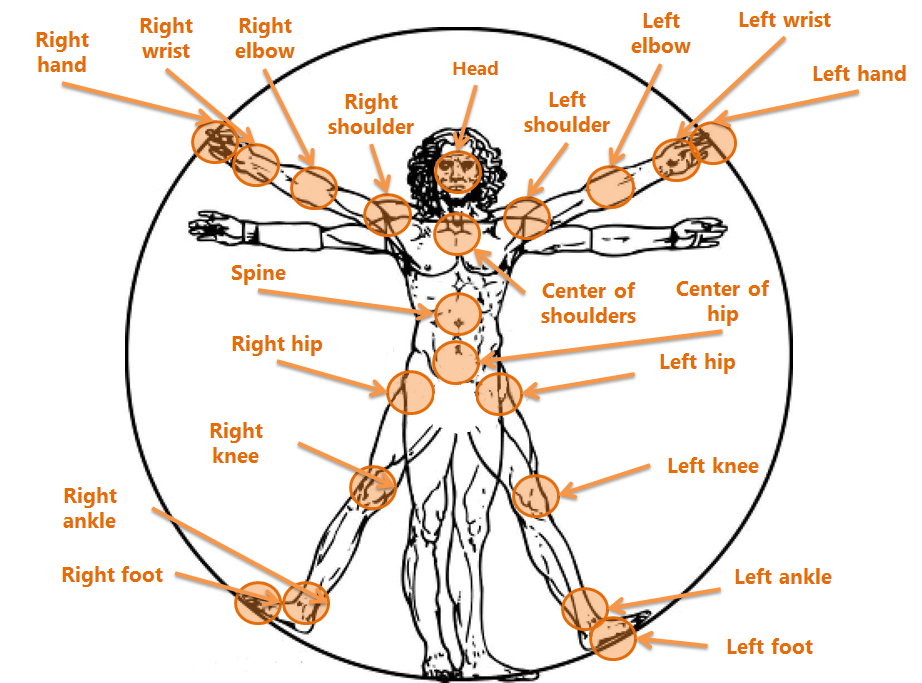
\includegraphics[scale=0.4]{./img/articulacoes.png}
 %% matrixargseg.png: 296x162 pixel, 100dpi, 7.52x4.11 cm, bb=0 0 213 117
 %%\caption{Estágio desenvolvimento de jogos ~\cite{fullerton2008game}}
%\caption[Posições das Articulações do Corpo Humano Adquiridas Pelo MS-Kinnect]{\copyright Posições das Articulações do Corpo Humano Adquiridas Pelo MS-Kinnect ~\cite{kinnect2013}}
%%  \caption{Estágio desenvolvimento de jogos}
 %\label{fig:articulacoeskinnect}
%\end{figure}
\begin{figure}[!h]
 \centering
 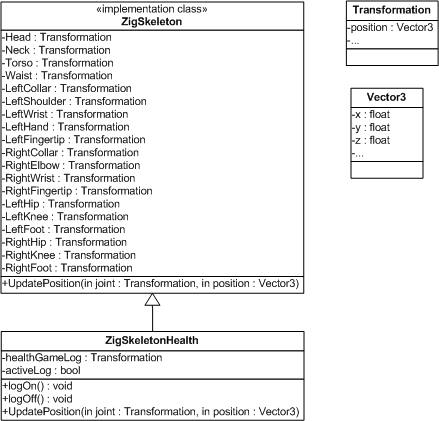
\includegraphics[scale=0.8]{./img/diagclasszigfu.png}
 \caption{Diagrama de Classe do ZigSkeleton e ZigSkeletonHealth}
 \label{fig:diagramaclassezigfu}
\end{figure}

O Zigfu ~\cite{zigfu} é um componente de software que permite integrar o Ms-Kinnect ao Unity3D. O Zigfu faz um mapeamento das articulações adquiridas pelo Ms-Kinnect, para uma classe chamada \textit{ZigSkeleton}, com todas as articulações, como podemos ver no Diagrama de Classe (Figura~\ref{fig:diagramaclassezigfu}). No entanto, para adquirir os sinais motores, é necessário armazenar os valores das posições das articulações durante as ações dos usuários. Por esse motivo, o Zigfu foi extendido na classe \textit{ZigSkeletonHealth} para armazenar as posições das articulações, além de um mecanismo para habilitar ou desabilitar o monitoramento dos sinais (métodos \textit{logOn() e logOff()}).


\subsubsection{Jogo: \textit{Catch the Spheres}}\label{jogo_catch}
Para testar a abordagem~\ac{jogue-me}, foi criado o jogo \textit{Catch the Spheres}, de acordo com os requisitos propostos na Seção~\ref{section:requisitos_solucao}.  

O \textit{Catch the Spheres} é um jogo em terceira pessoa, em que o jogador, por meio de seu personagem, deve tocar ou desviar das bolas que vêm em sua direção. Se o jogador tocar as bolas azuis, receberá uma pontuação por isso; caso seja atingido pelas bolas vermelhas, haverá uma penalização([REQ-JOGUE-ME-01]). Com o progresso do usuário, as bolas tornam-se mais rápidas, exigindo uma maior agilidade nos movimentos ([REQ-JOGUE-ME-02]). Este é o principal mecanismo de fluxo do jogo~\cite{sweetser2005-gameflow}, que tem o intuito de atrair a atenção do jogador, baseado nos desafios propostos ([REQ-JOGUE-ME-03]). 

Houve uma preocupação com a integridade física do jogador ([REQ-JOGUE-ME-04]). Por este motivo, baseado nos relatos dos usuários (Seção~\ref{gqm_usuarios}), o mecanismo de desvio de bolas foi removido por ter sido considerado inseguro.

\begin{figure}[!h]
     \centering
     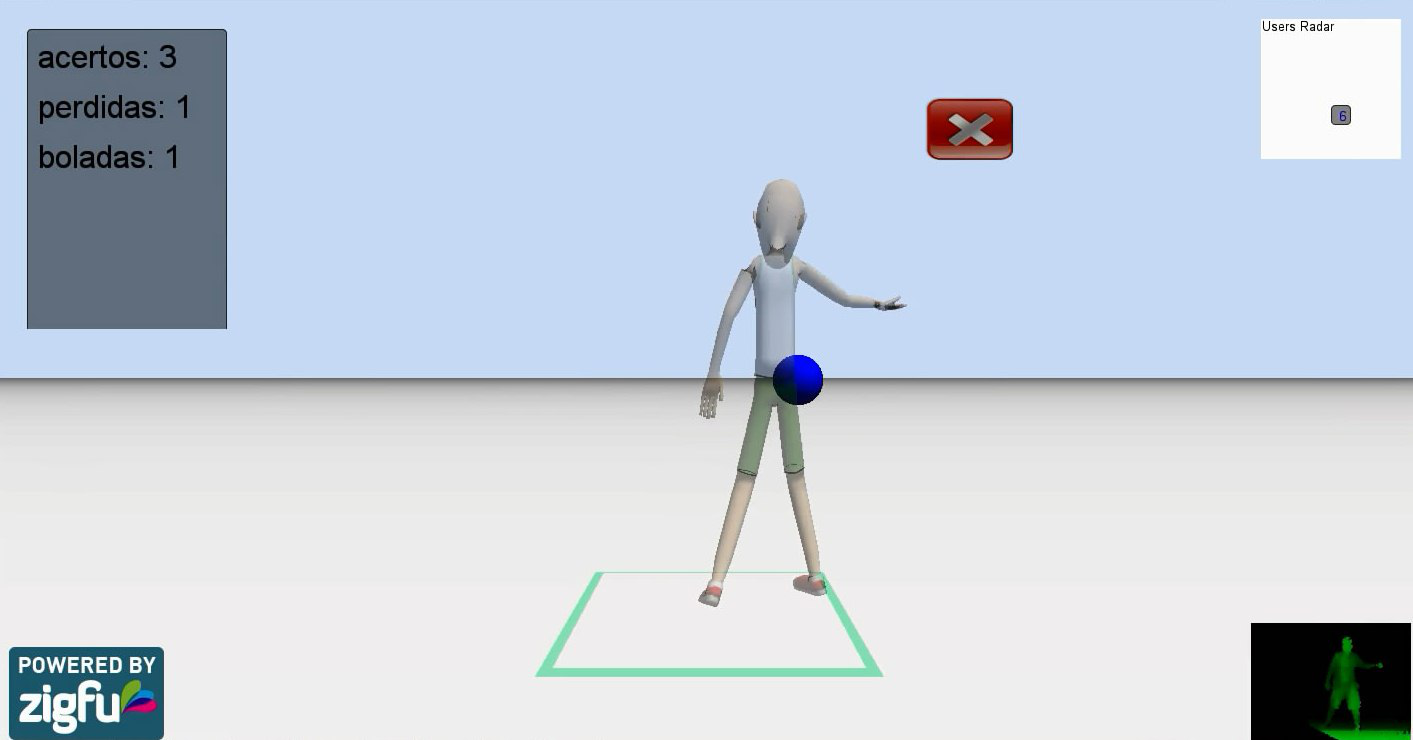
\includegraphics[width=.8\textwidth]{./img/catch-the-spheres.png}
     \caption{O jogo \emph{Catch the Spheres}}
     \label{img:catch}
\end{figure}

O mecanismo de aquisição e armazenamento dos sinais motores ([REQ-JOGUE-ME-05]) torna possível o envio de sinais motores de maneira colaborativa, usando um serviço responsável por receber e armazenar esses sinais. Na abordagem~\ac{jogue-me}, o servidor irá processar os sinais e transformá-los em informação para o profissional de saúde responsável pelo paciente.

\subsection{Arquitetura do \textit{JOGUE-ME Webservice}}
O mecanismo de aquisição e armazenamento dos sinais motores ([REQ-JOGUE-ME-05]) torna possível a análise dos dados motores do usuário no qual o jogo armazena as informações e as envia para o servidor de dados. 

O \textit{JOGUE-ME Webservice} é responsável por: criar usuário, receber dados motores, gerenciar arquivos exportá-los para o MATLAB~\cite{matlab2011} conforme a arquitetura descrita do Diagrama de Classes (Figura~\ref{fig:classd}).

\begin{figure}[!h]
     \centering
     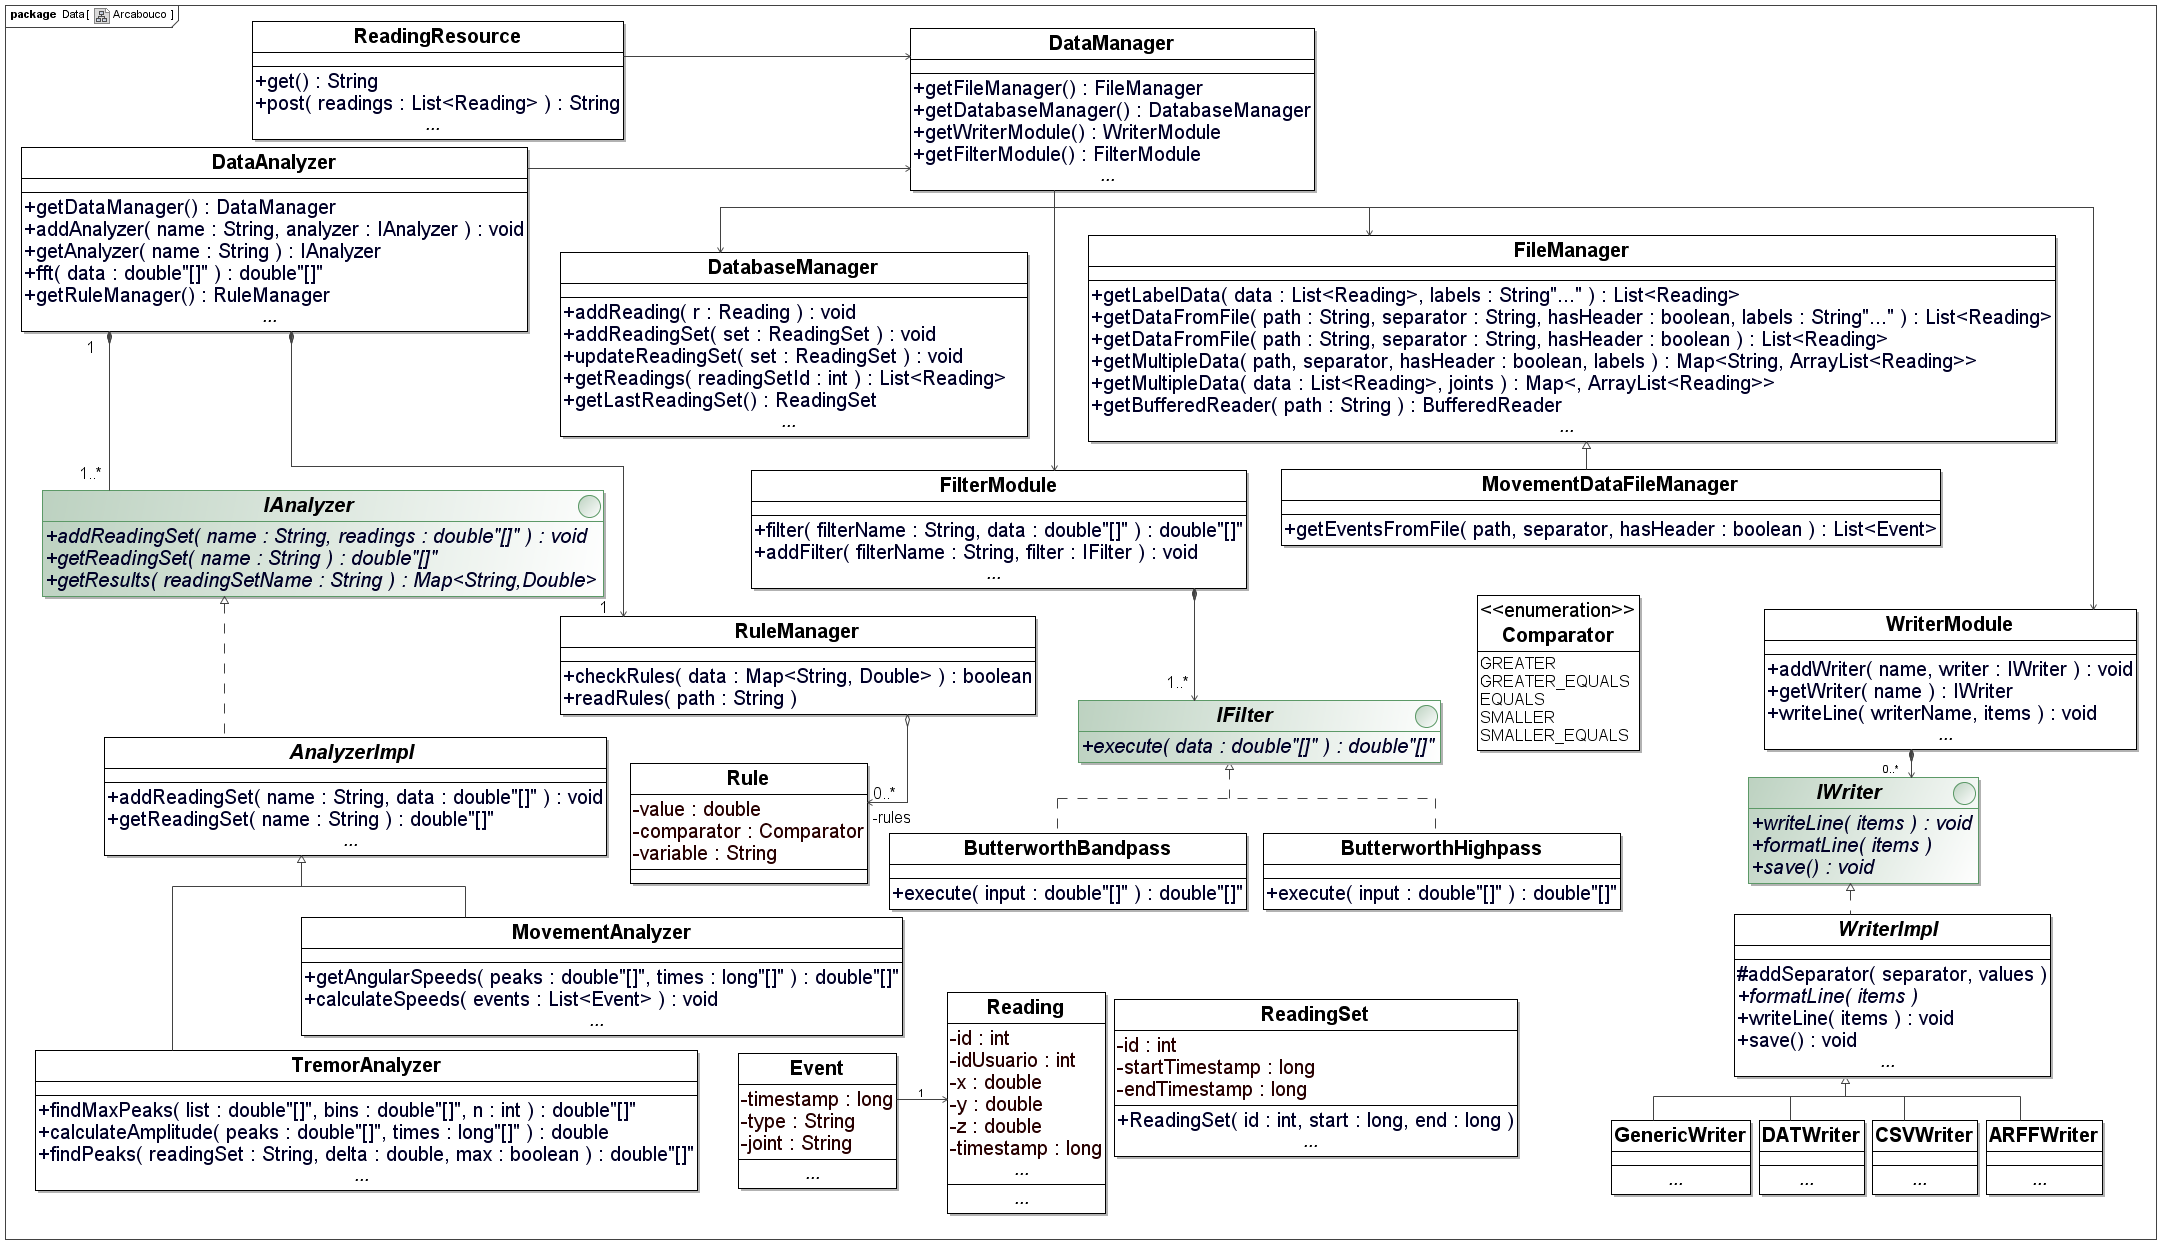
\includegraphics[width=1\textwidth]{./img/class_diagram.png}
     \caption[Diagrama de Classes do Serviço JOGUE-ME]{Diagrama de Classes do do Serviço JOGUE-ME}
     \label{fig:classd}
\end{figure}

O processo inicia com a aquisição dos dados dos sensores, que podem ser enviados para o \emph{webservice} e processados pela classe \texttt{ReadingResource} ou enviados por arquivos e processados pela classe \texttt{FileManager}, acessada através do \texttt{DataManager}. O \texttt{ReadingResource} envia os dados recebidos para o \texttt{DatabaseManager}, também acessado através do \texttt{DataManager}, para armazená-los no \emph{banco de dados} ~\cite{antonio2013}. Na Tabela~\ref{tab:operations}, ilustram-se as operações disponibilizadas pelo \textit{webservice} e um exemplo de como os dados devem ser estruturados para cada operação.

O envio dos dados dos usuários coletados com os dispositivos é feito através de uma requisição POST para o \textit{web service}. Os dados devem ser coletados durante uma sessão completa do jogo, que dura de alguns segundos a alguns minutos, para depois serem estruturados e enviados para o \textit{webservice}. O formato aceito pelas operações é o JSON (JavaScript Object Notation). 

\begin{table} 
\centering 
\caption{Operações disponibilizadas pelo \textit{web service}}
\begin{center}
    \begin{tabular}{ | l | c | l | }
        \hline
        Operação & Método & Exemplo \\ \hline
        cadastrarUsuario & POST & 
		\begin{minipage}{7cm}\begin{verbatim}
		
		{"id":2,"nome":"Ana",
		"masculino":false,
		"nascimento":"2012-11-28"}
		
		\end{verbatim}\end{minipage} \\ \hline
        obterToken & GET & - \\ \hline
        enviarDados & POST & 
		\begin{minipage}{7.5cm}\begin{verbatim}

		{"leitura":[{"id":0, 
		"idUsuario":1, "x":2.9097333, 
		"y":6.770132, "z":2.0355952, 
		"timestamp":1336134935706}, 
		{"id":0, "idUsuario":1, 
		"x":4.5565815, "y":4.9461093, 
		"z":1.4911331, 
		"timestamp":1336134935706}]}
		
		\end{verbatim}\end{minipage} \\ \hline
    \end{tabular}
\end{center}
\label{tab:operations}
\end{table}

\subsubsection{Gerenciador de Dados}
O \emph{Gerenciador de Dados} possui submódulos responsáveis por ler, separa e filtrar os dados, além do gerenciá-los usando um Banco de Dados para o armazenamento das informações motoras. A classe \texttt{DataManager} implementa as funcionalidades do \emph{Gerenciador de Dados}, referenciando os quatro módulos: \emph{Gerenciador de Arquivos}, \emph{Módulo de Escrita}, \emph{Módulo de Filtragem} e \emph{Gerenciador do Banco de Dados}. Estes módulos serão explicados nas subseções a seguir. A classe \texttt{DataManager} possui um construtor \texttt{DataManager(DatabaseManager, FileManager, WriterModule, FilterModule)}, que recebe como parâmetros os quatro módulos. Dessa forma, é possível aumentar a funcionalidade de cada um dos módulos estendendo suas respectivas classes por herança e adicionando a elas novos métodos. A classe \texttt{MovementDataFileManager}, tratada mais adiante, é um exemplo de extensão do \texttt{FileManager}.

O \emph{webservice}, implementado utilizou a biblioteca Jersey\footnote{Disponível em: http://jersey.java.net/}, que facilita o desenvolvimento de \textit{RESTful webservices}. As requisições são enviadas para serem processadas pela classe \texttt{ReadingResource}, que é um \textit{web resource}, uma entidade que recebe requisições HTTP e envia respostas. Esta classe possui dois métodos, o \texttt{get()} que trata requisições \emph{GET}, retornando o identificador do último conjunto de leituras para controle do armazenamento no banco de dados; e o método \texttt{post(List<Reading> readings)} processa os dados das leituras enviados através de requisições \emph{POST}, e convertidos de JSON para objetos Java pela biblioteca Jersey. A classe \texttt{ReadingResource} está acoplada à classe \texttt{DataManager} e, através dela, tem acesso ao \emph{Gerenciador do Banco de Dados}. O \emph{webservice} pode ser instalado em qualquer \textit{web container}, como o Apache Tomcat\footnote{Disponível em: http://tomcat.apache.org/} e o GlassFish\footnote{Disponível em: http://glassfish.
java.net/}.

\subsubsection{Gerenciador de Arquivos}

A classe \texttt{FileManager} implementa o módulo \emph{Gerenciador de Arquivos}, que processa as operações de abertura de arquivos de dados delegadas pelo \emph{Gerenciador de Dados}. Esse módulo processa os dados recebidos, armazenando-os em dados estruturados para serem processado posteriormente pelo \emph{Analisador de Dados}. O dado estruturado aceito pelo \emph{Analisador de Dados} é composto por um rótulo identificador do dado, uma marca de tempo com precisão de milissegundos, e coordenadas x, y e z, cujo significado depende do tipo de sensor que as gera.

Os métodos da classe \texttt{FileManager} são:
\begin{enumerate}
	\item \texttt{getLabelData(List<Reading> data, String... labels)} filtra os dados da lista de leituras \texttt{data}, retornando uma nova lista \texttt{List<Reading>} contendo apenas os dados com os rótulos definidos em \texttt{labels}.
	\item \texttt{getDataFromFile(String path, String separator, boolean hasHeader)} lê os dados de um arquivo localizado no caminho \texttt{path}, cujos dados estão separados pelo separador \texttt{separator} e definidos linha a linha. O parâmetro \texttt{hasHeader} indica se o método deve procurar por uma linha de cabeçalho na primeira linha do arquivo. Retorna uma \texttt{List<Reading>} com os dados.
	\item \label{getdatamethod} \texttt{getDataFromFile(String path, String separator, boolean hasHeader, String... labels)} estende a funcionalidade do método anterior, retornando uma \texttt{List<Reading>} com os dados que possuem os rótulos definidos em \texttt{labels}.
	\item \texttt{getMultipleData(String path, String separator, boolean hasHeader, String... labels)} possui a mesma função que o método~\ref{getdatamethod}, mas, diferente deste, retorna um \texttt{Map<String, List<Reading>>} onde cada chave do mapa é um rótulo e indexa uma lista de eventos identificados pelo rótulo.
	\item \texttt{getBufferedReader(String path)} retorna um \texttt{BufferedReader} para manipular o arquivo cujo caminho é especificado dem \texttt{path}.
\end{enumerate}

A classe \texttt{MovementDataFileManager} estende as funcionalidades do \texttt{FileManager}, adicionando um método para leitura de eventos oriundos de jogos. Os eventos marcam o início ou fim de um momento específico do jogo no qual o jogador estará executando um movimento que será enviado para análise.

\subsection{Módulo de Escrita}

O \emph{Módulo de Escrita} é implementado pela classe \texttt{WriterModule}, que é responsável pela saída dos dados processados pelo \emph{Analisador de Dados}. Os dados podem ser estruturados para serem mostrados em um programa de plotagem de gráficos, como o GNUPlot\footnote{Disponível em: http://www.gnuplot.info/}, ou para servirem como entrada para mecanismos de aprendizado de máquina. Os dados são escritos em CSV (\textit{Comma-separated Values}) ou em qualquer outro formato definido pelo usuário do arcabouço. O módulo de escrita também suporta a escrita de arquivos ARFF, para serem processados pelo Weka\footnote{Disponível em: http://www.cs.waikato.ac.nz/ml/weka/}. O \emph{Módulo de Escrita} é extensível para permitir a geração de um formato de arquivo específico. A criação de um novo arquivo de dados é feita através da extensão da classe \texttt{WriterImpl} pela classe que se está criando.

A interface \texttt{IWriter} define três métodos para manipular arquivos de dados:

\begin{enumerate}
	\item \label{formatlinemethod} \texttt{formatLine(Object... items)} formata os itens \texttt{items} adicionando separadores ou qualquer outra formatação adicional definida na classe específica de escrita que implementa \texttt{IWriter} ou estende \texttt{WriterImpl}.
	\item \texttt{writeLine(Object... items)} escreve uma nova linha no arquivo, seguindo a formatação definida pelo método~\ref{formatlinemethod}.
	\item \texttt{save()} fecha a \textit{stream} de escrita dedicada ao arquivo e salva o arquivo em disco.
\end{enumerate}

A classe \texttt{WriterImpl} implementa os métodos comuns a todas as classes de escrita, definidos pela interface \texttt{IWriter}, fornecendo um método adicional para incluir separadores entre os elementos de uma linha. Para definir um comportamento diferente daquele implementado por \texttt{WriterImpl}, deve-se implementar diretamente a interface \texttt{IWriter}.



%O \textit{JOGUE-ME Webservice} foi desenvolvido em colaboração com Antônio Santos Jr. em sua dissertação de mestrado ~\cite{antonio2013}. Do arcabouço do \textit{webservice} definido em seu trabalho, foram aproveitados os módulos de criação de usuário, recebimento de dados, gerenciador de arquivos e o módulo de escrita para gerar os arquivos a serem exportados e processados no MATLAB 2011 ~\cite{matlab2011} conforme a Arquitetura.

% \begin{figure}[!htb]
%      \centering
%      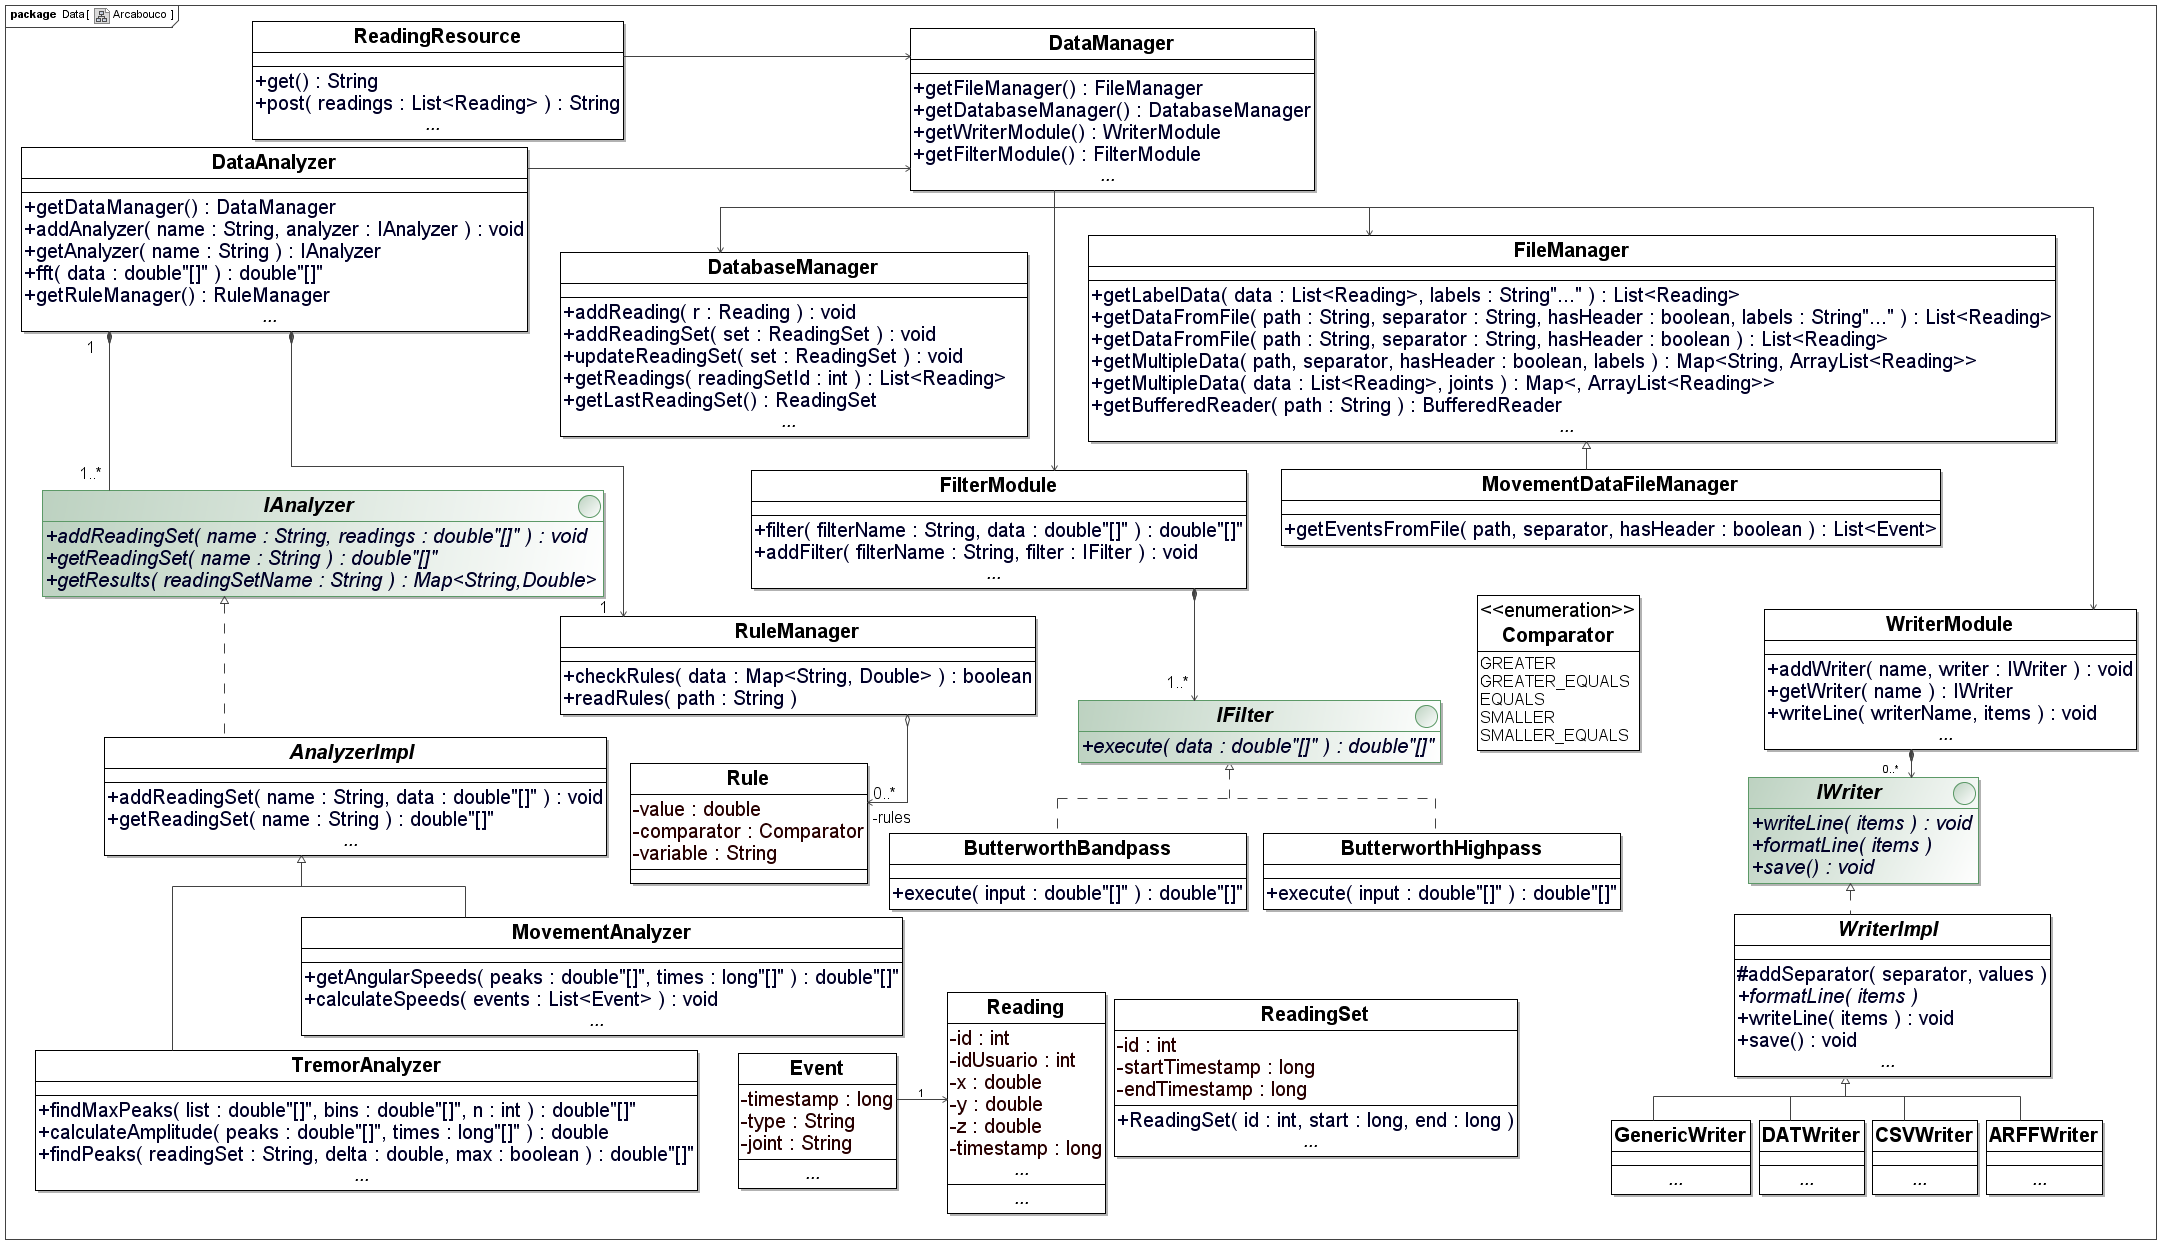
\includegraphics[width=1\textwidth]{./img/class_diagram.png}
%      \caption[Diagrama de Classes do Arcabouço]{Diagrama de Classes do Arcabouço ~\cite{antonio2013}}
%      \label{img:classd}
% \end{figure}

%O processo inicia com a aquisição dos dados dos sensores, que podem são enviados para o \emph{webservice} e processados pela classe \texttt{ReadingResource} ou enviados por arquivos e processados pela classe \texttt{FileManager}, acessada através do \texttt{DataManager}. O \texttt{ReadingResource} envia os dados recebidos para o \texttt{DatabaseManager}, também acessado através do \texttt{DataManager}, para armazená-los no \emph{banco de dados} ~\cite{antonio2013}. Na Tabela~\ref{tab:operations}, ilustram-se as operações disponibilizadas pelo \textit{webservice} e um exemplo de como os dados devem ser estruturados para cada operação.

%Os usuários enviam seus sinais, utilizando um cliente ~\ac{jogue-me} através de uma requisição \textit{POST}. Essa requisição é enviada no momento da finalização do jogo.
% 
% \begin{table} 
% \centering 
% \caption{Operações disponibilizadas pelo \textit{web service}}
% \begin{center}
%     \begin{tabular}{ | l | c | l | }
%         \hline
%         Operação & Método & Exemplo \\ \hline
%         cadastrarUsuario & POST & 
% 		\begin{minipage}{7cm}\begin{verbatim}
% 		
% 		{"id":2,"nome":"Ana",
% 		"masculino":false,
% 		"nascimento":"2012-11-28"}
% 		
% 		\end{verbatim}\end{minipage} \\ \hline
%         obterToken & GET & - \\ \hline
%         enviarDados & POST & 
% 		\begin{minipage}{7.5cm}\begin{verbatim}
% 
% 		{"leitura":[{"id":0, 
% 		"idUsuario":1, "x":2.9097333, 
% 		"y":6.770132, "z":2.0355952, 
% 		"timestamp":1336134935706}, 
% 		{"id":0, "idUsuario":1, 
% 		"x":4.5565815, "y":4.9461093, 
% 		"z":1.4911331, 
% 		"timestamp":1336134935706}]}
% 		
% 		\end{verbatim}\end{minipage} \\ \hline
%     \end{tabular}
% \end{center}
% \label{tab:operations}
% \end{table}

\section{Processador de Dados Biomecânicos}\label{sec:processador_bio}
Para transformar os sinais em informação, tanto para o profissional de saúde, quanto para máquinas de aprendizagem, é necessário fazer o processamento desse sinal. Neste trabalho, foi implementado o \textit{Processador de Dados Biomecânicos} em MATLAB 2011~\cite{matlab2011}. Este processador consiste de três passos: Identificação dos Ciclos, Extração de Características e Filtragem de Dados.

\subsection{Identificação dos Ciclos de Movimento} 
A identificação dos ciclos de movimento foi baseada na identificação de picos e vales do sinal motor, como explicado na Seção~\ref{section:identificao_ciclos}. 

Para implementar o mecanismo de detecção de ciclos, fez-se o uso da biblioteca \textit{Peak Detection in Matlab}~\cite{peakdetect}. Essa biblioteca possui uma função chamada \textit{peakdet()}, que recebe como parâmetros um vetor contendo o sinal a ser processado e um valor de limiar para remoção do ruído do sinal. A função retorna dois vetores: um possui os valores das máximas (picos) e o outro retorna os valores das mínimas (vales).

Usando a função \textit{peakdet()}, criou-se a função \textit{cycleperiodic()}, que tem o objetivo de identificar os ciclos periódicos de um sinal. Foram adicionados dois parâmetros a essa função, para justamente levar em consideração as amplitudes máximas e mínimas permitidas por este sinal.

%\begin{lstlisting}[frame=single, caption=Função de Ciclo Periódico]  % Start your code-block
%
%function [cycleIndex]=cycleperiodic(v, delta, maxAmplitude, minAmplitude)
%[peaks, valey] = peakdet(v, delta);
%j = 1;
%for (i=1:(size(valey,1)-1))    
    %initialIndex = valey(i,1);
    %endIndex = valey(i+1,1);
    %amplitude = endIndex - initialIndex;
    %if ((maxAmplitude >= amplitude) & (minAmplitude <= amplitude))
        %cycleIndex(j) = valey(i);
        %j = j +1;
    %end
%end
%\end{lstlisting}

De posse dos ciclos, pôde ser identificado quando começam e terminam os movimentos periódicos (Código Fonte~\ref{lst:identifyCycles}), como, por exemplo, os movimentos sucessivos de adução e abdução do braço (Seção ~\ref{fig:movabducaoaducao}). 

\begin{lstlisting}[frame=single, caption=Identificar Início e Tamanho do Movimento Periódico, label=lst:identifyCycles]  % Start your code-block

function [WindowBeginLeft, WindowLengthLeft, WindowBeginRight, WindowLengthRight] = identifyCycles(leftWristJoint, rightWristJoint)
    signalLeft = leftWristJoint(:,3);
    signalRight = rightWristJoint(:,3);

    cycleIndexLeft = cycleperiodic(signalLeft, 500, 200, 40);
    cycleIndexRight = cycleperiodic(signalRight, 500, 200, 40);

    WindowBeginLeft = cycleIndexLeft(1);
    WindowLengthLeft = cycleIndexLeft(size(cycleIndexLeft,2));
    WindowBeginRight = cycleIndexRight(1);
    WindowLengthRight = cycleIndexRight(size(cycleIndexRight,2));
\end{lstlisting}

\subsection{Extração das Características do Movimento}
Supondo que os ciclos de movimento foram identificados através da posição do punho, é necessário extrair as características do movimento. Para isso, o primeiro passo é calcular os ângulos relativos do movimento angular, usando os pontos das articulações, como pode ser visto no Código Fonte~\ref{lst:calculate_angle}. Então, a função \textit{ArmRelativeAngleTorso()} realiza o cálculo do produto escalar entre as três articulações.

\begin{lstlisting}[frame=single, caption=Calcular ângulos relativos do movimento, label=lst:calculate_angle]
leftShoulderJoint = leftShoulderJoint(WindowBeginLeft:WindowLengthLeft,:);
leftWristJoint = leftWristJoint(WindowBeginLeft:WindowLengthLeft,:);  
leftHipJoint = leftHipJoint(WindowBeginLeft:WindowLengthLeft,:);  

for (j=1:size(leftHipJoint,1))
leftArmAngle(j,1) = leftHipJoint(j,1);
        

leftArmAngle(j,2) = ArmRelativeAngleTorso(leftHipJoint,leftShoulderJoint,leftWristJoint, j);    
end
\end{lstlisting}

De posse do sinal dos ângulos relativos do movimento, são extraídos os picos e os vales desse sinal para calcularmos a velocidade angular do movimento de abdução e adução do braço (Código Fonte: ~\ref{lst:angular_velocity}).
    
\begin{lstlisting}[frame=single, caption=Calcular Velociodade Angular Adução e Abdução, label=lst:angular_velocity]	
distanceup = cycle(peak) - cycle(1);
amplitude(identifiedCycles,1) = cycle(peak);
    
timestampupsec = (abs(timestampcycle(1) - timestampcycle(peak)))/1000;
velocityUp(identifiedCycles,1) = distanceup/timestampupsec;

distancedown = abs(cycle(end) - cycle(peak));
timestampdownsec = (abs(timestampcycle(peak) - timestampcycle(end)))/1000;
velocityDown(identifiedCycles,1) = distancedown/timestampdownsec;
\end{lstlisting}	
		
\subsection{Filtro de Dados}
O filtro de dados remove os ciclos de movimento incompletos ou com problemas na aquisição dos dados, como explicado na Seção~\ref{section:filtro_dados}. Nessa etapa, os ciclos são normalizados, escalonados e rotulados por usuário. 
De posse de todos os dados, é calculado um vetor médio dos ciclos normalizados, para definir um limiar (\textit{threshold}) de remoção dos ciclos (Código Fonte:~\ref{code:filtercycles}).

	\begin{lstlisting}[frame=single, caption=Calcular Velociodade Angular Adução e Abdução, label=code:filtercycles]
function [ KinnectData, processedCycles, labels ] = filterCyclesAndLabels (T, labels, otherFeatures, scaledLength)

    normalization = T;
    for i=1:size(T,1)
       normalization(i,1:scaledLength) = T(i,1:scaledLength)./max(T(i,1:scaledLength));
       normalization(i,scaledLength+1:scaledLength*2) = T(i,scaledLength+1:scaledLength*2)./max(T(i,scaledLength+1:scaledLength*2));
       normalization(isnan(normalization(i,1:scaledLength*2))) = min(normalization(i,1:scaledLength*2));
    end
    
    normalization(isnan(normalization)) = 0;
    
    if(size(T,2) > scaledLength*2) 
       normalization(:,scaledLength*2 + 1:end) =  T(:,scaledLength*2+1 : end)./max(T(:,scaledLength*2 + 1:end));
    end
    
    threshold = 1;
    meanOfNormalization = mean(normalization);
    u = ones(size(normalization,1),1);
    filterTestVector = sum((normalization - (u*meanOfNormalization)).^2,2);
    filterVector = filterTestVector<threshold;
    
       
    KinnectData = [T(filterVector,:) otherFeatures(filterVector,:)];
    processedCycles = T(filterVector,:);
    labels = labels(filterVector,:);    
end
\end{lstlisting}	


\section{Classificador de Dados}
Para avaliar os requisitos de identificação dos sinais motores ([REQ-JOGUE-ME-06]), é necessário um teste com seres humanos, para avaliar a aquisição e a classificação dos sinais. A abordagem de classificação dos dados é baseada em máquinas de aprendizagem, como explicado na Seção~\ref{section:class_dados}. O Código Fonte~\ref{code:classification} demonstra como fazer a classificação dos dados utilizando o \textit{Matlab Statistics Toolbox}~\cite{matlab2011}, que possui um~\ac{svm} disponível em sua biblioteca.

Primeiramente, separa-se o grupo de treinamento para realizar a aprendizagem da máquina, utilizando o método \textit{svmtrain()}; depois utiliza-se o método \textit{svmclassify()} para predizer os valores usando esta máquina de aprendizagem; por fim, calculam-se as diferenças entre os valores reais. Então, é calculada a taxa de erro para avaliar o resultado do classificador.

\begin{lstlisting}[frame=single, caption=Uso de Máquina de Vetor de Suporte para Classificação dos Dados, label=code:classification]
realValues; %Classe Atual
SVMStruct = svmtrain(trainingData,trainningClassification,'Kernel_Function', 'linear',	'BoxConstraint', 0.10);
class = svmclassify(SVMStruct, testData, 'showplot',true); %Classe Preditiva
classificationRate = sum(class~=realValues);
errorRate = classificationRate/size(classereal,2);
\end{lstlisting}

\section{Conclusão}
Neste capítulo foram apresentados os passos da implementação de um~\ac{jogue-me} para o monitoramento do sinal da bradicinesia presente no~\ac{dp}. 

Foi apresentado o design da arquitetura tanto do cliente quanto do serviço de recebimento de requisições, processamento do sinal e identificação do sintoma da bradicinesia~\cite{protpar010} presente no~\ac{dp}. Demonstrou-se neste capítulo detalhes da implementação para que este trabalho possa ser replicado para outras análises motoras.

No capítulo seguinte, é apresentado os experimentos realizados para avaliar este trabalho referentes a: perspectiva do profissional de saúde e suas necessidades, resultado da identificação do sintoma da bradicinesia no estudo analítico de caso-controle e a avaliação dos pacientes com parkinson quanto à proposta de monitoramento dos sinais motores usando jogos eletrônicos.


%Para reaplicar esta implementação em outros~\ac{sms}  Esta arquitetura pode ser reaplicada em outros contextos, mas como vimos na Seção	
\chapter{Avalia\c{c}\~{a}o Experimental} \label{chap:avaliacao}
A realização do monitoramento dos sinais motores, de uma maneira não invasiva, é um desafio. Logo, esta tese fornece uma forma lúdica de monitorar os dados de saúde, por meio de jogos eletrônicos que podem ser integrados à rotina diária dos usuários. Neste capítulo, iremos demonstrar que conseguimos desenvolver um~\ac{sms} não invasivo para monitoramento de um sinal do~\ac{dp} com uma taxa de acurácia de 86,67\%.

%Pois, a partir de um \textit{HGMS-E} é possível capturar, processar e classificar os movimentos cinéticos exercidos pelos usuários.

%Sabendo que o acompanhamento de sinais motores, integrados à rotina diária do paciente traz benefícios ao tratamento e qualidade de vida do mesmo do ponto de vista do profissional da saúde. Por intermédio desse trabalho, conseguimos capturar dados motores utilizando sensores de movimento. Esses dados permitem auxiliar no acompanhamento de doenças com comprometimento motor tal como o~\ac{dp}. Então, neste trabalho nós desenvolvemos um mecanismo de de captura de dados motores embutidos num jogo eletrônico, o qual permite monitorar e quantificar os sinais motores de uma forma lúdica e não-invasiva.




\section{ETAPA 1 - Entrevista Semiestruturada com Profissionais de Saúde}\label{sec:entrevista_semi_estruturada}



A interpretação de dados é o cerne da pesquisa qualitativa, tem como função desenvolver a teoria e servir, ao mesmo tempo, de base para a decisão sobre quais dados adicionais devem ser coletados, por meio de codificação seletiva~\cite{FLI04}. Esta técnica permite elaborar uma categorização nos dados e demonstrar ao pesquisador quais são os fenômenos mais preponderantes da pesquisa. O procedimento da interpretação dos dados, assim como a integração de material adicional, são encerrados quando se atinge a "saturação teórica", ou seja, quando o avanço na codificação não resulta na aquisição de novos conhecimentos~\cite{FLI04}.

Para análise dos textos provenientes da pesquisa, foram transcritos as entrevistas com neurologistas e fisioterapeutas especialistas em neurologia. Com  a codificação seletiva, foi possível categorizar as ocorrências de acordo com o conteúdo de cada texto. Ou seja, as respostas de cada participante foram analisadas e incluídas na árvore de categorias como sugere o método de pesquisa~\cite{FLI04}. 

Para auxiliar no processo de análise, seleção e codificação, foi utilizado uma ferramenta de suporte à pesquisa qualitativa (\textit{QDA Miner}~\cite{qda13}) e, por meio desta, foi possível categorizar e reformular a árvore de categorias~\cite{FLI04} diversas vezes durante o processo de análise~\cite{FLI04}.


\subsection{Objetivo da Entrevista Semiestruturada}
O objetivo da entrevista semiestruturada~\cite{FLI04} foi entender como é feito o acompanhamento do paciente com sintomatologia do~\ac{dp}, juntamente aos profissionais de saúde: neurologistas, que prescrevem a dosagem medicamentosa, e fisioterapeutas, que fazem o tratamento de reabilitação e acompanhamento motor do paciente. Esses profissionais de saúde foram indagados se haveria melhora na tomada de decisão, caso estes pudessem acompanhar os sinais motores diariamente. Procurou-se encontrar, dentro do contexto de estudo, a importância do monitoramento de dados de saúde e os benefícios trazidos por este.

As entrevistas foram realizadas presencialmente, com perguntas não estruturadas e com uma maior estruturação no decorrer da entrevista, preocupando-se em evitar a referência do entrevistador sobre os pontos de vista do entrevistado, conforme sugere o método científico~\cite{FLI04}. 

\subsubsection{Instrumento de Análise dos Dados da Pesquisa Qualitativa} \label{section:analise_dados} 
A pesquisa qualitativa assistida por computador permite uma melhor categorização das informações obtidas em modo texto. O \textit{software} QDA Miner~\cite{qda13} auxilia o pesquisador na organização dos registros da pesquisa e em suas interpretações, justificando-se o uso da ferramenta devido à dificuldade de classificar e analisar os dados obtidos. Nessa análise, foram consideradas as atividades referentes ao acompanhamento dos sinais motores em pacientes com~\ac{dp}. Buscou-se, durante a pesquisa, avaliar se um cenário de monitoramento dos sinais motores, por meio de jogos eletrônicos, auxiliaria os profissionais de saúde quanto ao tratamento de seus pacientes.

Nesta seção, faz-se um detalhamento do resultado da entrevista semiestruturada, que descreve a opinião dos entrevistados, e coleta-se requisitos baseados em suas necessidades, devidamente expostas. Por meio desta entrevista, foi avaliada a \textbf{ETAPA 1}: \textit{Quais os benefícios de acompanhar os sinais motores do paciente diariamente, do ponto de vista do profissional da saúde?}

%	\begin{description}

%	\item[H1] O acompanhamento de sinais motores integrados à rotina diária do paciente, traz benefícios ao tratamento e na qualidade de vida do mesmo, do ponto de vista do profissional da saúde.
% 	\end{description}
	
%\subsubsection{Análise da Entrevista Semi-Estruturada}
%A análise qualitativa ~\cite{FLI04} permite identificar as práticas dos profissionais de saúde referentes ao acompanhamento dos sinais motores em pacientes de parkinson e como essas práticas podem ser aperfeiçoadas num cenário em que haja o monitoramento dos sinais. 


\subsection{Perfil dos Participantes}
O perfil dos participantes é composto por quatro profissionais da saúde, dos quais dois são fisioterapeutas, com especialização em neurologia, e dois são médicos neurologistas. A escolha desse perfil se fez de acordo com seus ofícios, responsabilidades e complementaridade quanto ao tratamento do paciente. Os neurologistas realizam o diagnóstico e acompanham os sinais motores juntamente com as informações obtidas do paciente ou de seu cuidador, e, baseados nestas informações, realizam o gerenciamento da dosagem medicamentosa da doença. Por outro lado, os fisioterapeutas fazem o acompanhamento dos sinais motores em sessões de fisioterapia e promovem a reaprendizagem motora destes pacientes. Logo, esses profissionais possuem visões e preocupações distintas, inerentes ao seu ofício. 

Para manter a confidencialidade de informação, os entrevistados receberam uma \textbf{LEGENDA}, que identifica o perfil profissional seguido por um número sequencial, o qual identifica o entrevistado, mas preserva sua identidade (Tabela~\ref{table:perfil_analise_participantes}).

\begin{table}[h]
\caption{Perfil dos Participantes}
\label{table:perfil_analise_participantes}
\begin{tabular}{|l|l|c|c|}
\hline
\textbf{LEGENDA} & \textbf{PROFISSÃO}             & \multicolumn{1}{|l}{\textbf{IDADE (ANOS)}} & \multicolumn{1}{|l|}{\textbf{EXPERIÊNCIA (ANOS)}} \\ \hline
FIS\_01          & Fisioterapia em Neurologia & 40                                         & 10                                                \\ \hline
FIS\_02          & Fisioterapia em Neurologia     & 39                                         & 10                                                \\ \hline
NEU\_01          & Médico Neurologista            & 42                                         & 15                                                \\ \hline
NEU\_02          & Médico Neurologista            & 67                                         & 30                                                \\ \hline
\end{tabular}

\end{table}

\subsubsection{Questionário de Pesquisa}
Para a formulação do questionário, foram realizadas análises nas diretrizes médicas~\cite{protpar010,national2006parkinson} e na tabela UPDRS~\cite{updrs87}, sobre o progresso do~\ac{dp} e dos sinais monitoráveis por sensores de movimento. Para a entrevista, foram elaboradas 15 perguntas, agrupadas em 3 seções (Apêndice \ref{apendice:entrevista-semi-estruturada}), com os seguintes temas: sinais do~\ac{dp}, monitoramento da saúde motora e benefícios advindos do monitoramento. O entrevistador selecionou as questões de acordo com o perfil profissional.

\subsection{Análise}
Durante a análise das entrevistas, foram extraídos fragmentos, e a nomenclatura utilizada contém o prefixo \textbf{FRAGMENTO} mais um número sequencial identificando-o. Esse procedimento permite identificar \textbf{requisitos} que orientem a proposta de monitoramento de dados motores por intermédio de jogos eletrônicos. Logo, os requisitos extraídos nesta abordagem foram obtidos a partir da perspectiva do profissional de saúde em relação ao tratamento e ao acompanhamento do~\ac{dp}. 

\subsubsection{Diagnóstico}\label{section:analise_diagnostico}

Na entrevista junto aos neurologistas, foi indagado como o diagnostico do~\ac{dp} é realizado.  A entrevista corroborou com a literatura médica~\cite{tolosa06,vedolin2003} em relação ao diagnóstico de exclusão do \ac{dp}~\cite{protpar010,national2006parkinson}.  

Todos os profissionais informaram que o sintoma mais comum é o tremor de repouso, e que este é inicialmente unilateral, seguido de uma bradicinesia, como podemos perceber nos fragmentos ([FRAGMENTO-01], FRAGMENTO-02]). Ainda no ([FRAGMENTO-01]), existe uma ocorrência do \textbf{[NEU\_01]}, em que o mesmo evoca sobre a importância da técnica de \textit{Finger Taps} ~\cite{updrs87} para avaliação da bradicinesia.




\begin{quote}
\textbf{[FRAGMENTO-01][NEU\_01]} - 
\emph{
O diagnóstico da doença de Parkinson é dado, principalmente, quando o paciente chega se queixando de tremor. Esse sintoma começa com um tremor unilateral, geralmente, pelas mãos, lentamente progressivo e de repouso. Além do tremor, esse paciente exibe uma lentidão que detectamos pelo \textit{Finger Taps}. Essa técnica consiste em tocar o polegar no primeiro e no segundo dedo simultaneamente, para ver se há ou não lentidão. Faz-se uma comparação sempre com o outro lado para visualizar possíveis diferenças. Existe, também, uma rigidez no braço, quando faz-se uma flexão e extensão do membro e percebe-se que o tônus desse paciente, comparado com o outro lado, exibe uma diferença.
}
\end{quote}

\begin{quote}
\textbf{[FRAGMENTO-02][NEU\_02]} -
\emph{
O diagnóstico da doença de Parkinson é feito com uma das queixas iniciais do paciente: o tremor de repouso, associado  a dificuldade na marcha. Então, normalmente, os pacientes reclamam de uma perna presa e um tremor de repouso. 
}
\end{quote}

Uma ocorrência no ([FRAGMENTO-03]) que deve ser ressaltada é o que o entrevistado referiu como ``\textit{boa resposta ao prolopa}''. Essa ocorrência é denominada de diagnóstico diferencial do~\ac{dp} ~\cite{protpar010} e consiste na redução dos sinais parkinsonianos em decorrência da resposta ao tratamento medicamentoso. 

\begin{quote}
\textbf{[FRAGMENTO-03][NEU\_01]} - 
\emph{
Então, os sinais são: o tremor em repouso, lentidão e a rigidez. Apenas de um lado inicialmente, por exemplo, começa no braço direito e depois vai para a perna direita, depois para o braço esquerdo e depois a perna esquerda. Isso lentamente progressivo, fazemos a exclusão com outras doenças através de outros exames, como tomografia, ressonância ou uma boa resposta ao prolopa.
}
\end{quote}

\subsubsection{Sintomas}
Nesta seção, estão expostos sinais para o acompanhamento da sintomatologia do~\ac{dp}.

%\subsubsection{Tremor}
O sintoma de tremor, além de ter sido referenciado durante o diagnóstico da doença, na Seção ~\ref{section:analise_diagnostico}, por todos os entrevistados, possui particularidades, como a dificuldade de controlar o sintoma por intermédio do tratamento medicamentoso ([FRAGMENTO-04]), e não é tão incapacitante quanto a bradicinesia. No ([FRAGMENTO-05]), o [NEU\_01] reforçou sobre a importância de controlar os sinais de lentidão do movimento ante os de tremor~\cite{do2007parkinson}.

\begin{quote}
\textbf{[FRAGMENTO-04][NEU\_01]} - 
\emph{
Necessário observar porque o tremor é, as vezes, mais difícil de controlar, pois está relacionado ao emocional do paciente e, quanto mais emocionalmente desequilibrado o paciente tiver, mais tremor ele tem.
}
\end{quote}

\begin{quote}
\textbf{[FRAGMENTO-05][NEU\_01]} - 
\emph{
O controle do tremor é um pouco complicado, devido a dificuldade dominá-lo com as medicações existentes hoje. Então, você poderia ver nesse seu projeto a lentidão. Porque, o paciente poderá apresentar lentidão, porém o paciente quer tremer, mas não quer ficar lento.
}
\end{quote}


%\subsubsection{Bradicinesia}\label{section:analise_bradicinesia}

O pesquisador indagou se o sintoma da bradicinesia era considerado o mais debilitante do~\ac{dp}; como resposta, ele obteve a afirmação de que a bradicinesia impacta, diretamente, na qualidade de vida do paciente, privando-o de realizar atividades diárias ([FRAGMENTO-06]).

\begin{quote}
\textbf{[FRAGMENTO-06][NEU\_01]} - 
\emph{
É ele atrapalha né, principalmente no levantar, andar. Para você se levantar, pentear o cabelo, o tremor é prejudicial. Porém, mais prejudicial ainda, é a lentidão do movimento.
}
\end{quote}

Ao indagar se o movimento de adução e abdução do braço seria relevante para a identificação do~\ac{dp}, o [NEU\_01] informou que a bradicinesia é um sintoma que traz lentidão em todo o corpo e, possivelmente, seria afetada por este movimento, pois, devido à redução dos movimentos automáticos ([FRAGMENTO-07]), traz outros impactos físicos ao paciente ([FRAGMENTO-08]).

\begin{quote}
\textbf{[FRAGMENTO-07][NEU\_01]} - 
\emph{
Na verdade, o movimento da abdução demonstrará o quão lento está. Porque, o comprometimento na doença de Parkinson está no comprometimento piramidal. O comprometimento extra-piramidal não vai estar alterando a força motora. No entanto, o comprometimento piramidal irá impactar justamente na lentidão. Por exemplo, quando um paciente com~\ac{dp} está andando, percebe-se a redução dos movimentos automáticos, principalmente, no balançar dos braços. Ele vai andando, vai andando, e você percebe que o paciente que está com a força e com a estrutura piramidal normal. No entanto, anda lento em consequência da redução dos movimentos automáticos.
}
\end{quote}


\begin{quote}
\textbf{[FRAGMENTO-08][FIS\_01]} - 
\emph{
Os sinais mais frequentes a gente tem a bradicinesia que é a lentificação do movimento, a gente tem um padrão postural que começa a ficar bem nítido que o paciente apresentar o Parkinson. Você percebe uma perda da movimentação automática da cintura escapular e aí ele começa a apresentar uma diminuição no volume da voz que é uma diplofonia, e apresenta uma maior rigidez muscular. Eles reclamam bastante e a bradicinesia que tornam os movimentos cada vez mais lentos.
}
\end{quote}

%\subsubsection{Marcha}
% Foi identificada uma ocorrência na dificuldade do andar do paciente de~\ac{dp}, quando o [NEU\_01] cita no ([FRAGMENTO-07]) (``\textit{Você vai andando, vai andando, você vê aquele paciente que está com a força, ele está com toda a estrutura piramidal tudo normal. Mas ela anda lento em consequência da lentidão do movimento ...}''. O [NEU\_02] corrobora com a mesma opinião ao citar a dificuldade de iniciar a marcha no ([FRAGMENTO-09]). O fisioterapeuta no papel de realizar o acompanhamento da marcha nas sessões fisioterápicas, fornece um aprendizado motor para a melhora da qualidade de vida do paciente de acordo com suas limitações ([FRAGMENTO-10]).
% 
% \begin{quote}
% \textbf{[FRAGMENTO-09][NEU\_02]} - 
% \emph{
% Problema na marcha. Dificuldade de iniciar a marcha, certa dificuldade de um lado comprometido. Mesmo quando o sintoma está unilateral eles sentem dificuldade para iniciar a marcha.
% }
% \end{quote}
% 
% \begin{quote}
% \textbf{[FRAGMENTO-10][FIS\_01]} - 
% \emph{
% Numa marcha, o doente de Parkinson tem a tendência de estar olhando para o chão. Mas a gente sabe que isso não é compatível com uma boa marcha a tendência é cair, para piorar eles têm os passos miúdos e também um passo arrastado. Então esse passo favorece a queda, poise ele perdeu a marcha automática que é aquela que a gente adquire na infância. O que a gente faz nas sessões de fisioterapia é tentar aplicar auto-correções para adaptar o paciente à nova realidade para que ele tenha uma aprendizado motor e no futuro um automatismo do movimento.
% }
% \end{quote}
% 
% Devido a quantidade de ocorrências sobre a análise da marcha para o acompanhamento da ~\ac{dp}, e a possibilidade da ocorrência de quedas dos indivíduos. Esses, dois fatos corroboraram com o uso de base de dados contendo dados sobre a marcha, pois isto vai além do custo financeiro para a aquisição dos sensores que capturam a ~\ac{fvrs}. Logo, ao usar bases contendo esses dados para a pesquisa, preserva-se a integridade física dos pacientes.



\subsubsection{Monitoramento Motor}
Nesta seção, está exposta a importância do monitoramento dos sinais capturados no estudo analítico de caso controle, definido no método de pesquisa na Seção~\ref{section:estudo_caso_controle}. Nesse estudo, também pretende-se identificar as características dos movimentos que possam ser extraídos desses sinais, e que venham fornecer subsídios para diferenciar indivíduos diagnosticados com~\ac{dp} ante indivíduos sem o diagnóstico.

%\subsubsection{Amplitude do Movimento dos Braços}

Ao indagar ao [FIS\_02] se o movimento de adução e abdução do braço seria relevante para a identificação do~\ac{dp}, este informou que mesmo não sendo um teste específico para a identificação da doença, existem diferenças significativas encontradas em indivíduos diagnosticados com parkinson [FRAGMENTO-11].
\begin{quote}
\textbf{[FRAGMENTO-11][FIS\_02]}-
\emph{
Sim. Existe alterações sim, mas eu nunca vi especificamente esse teste como sendo usado para diagnóstico da doença. Mas que realmente existem mudanças no movimento de adução e abdução de uma pessoa normal ante a um parkinsoniano.
}
\end{quote}

O [FIS\_01] explicou os motivos que levam a perda da mobilidade no movimento de adução e abdução ([FRAGMENTO-12]) e, consequentemente, reforça que esse movimento poderia ser monitorado para verificar o comprometimento da doença. Em um outro fragmento ([FRAGMENTO-13]), o mesmo fisioterapeuta menciona a importância de monitorar a amplitude do movimento, pois permite visualizar a resposta do paciente ao tratamento oferecido.

\begin{quote}
\textbf{[FRAGMENTO-12][FIS\_01]}-
\emph{
Têm, porque uma das grandes perdas que eles apresentam é na cintura escapular e consequentemente é pegando a parte de ombro. Pois caso ela seja mais fixa, porque geralmente o paciente de Parkinson abduz o ombro. O ombro fica abduzido junto ao tronco e ai ele perde a mobilidade do cotovelo e punho e também o movimento fica comprometido por conta disso.
}
\end{quote}

\begin{quote}
\textbf{[FRAGMENTO-13][FIS\_01]}-
\emph{
Mesmo sabendo que a tendência é uma lentificação (bradicinesia).  As outras doenças também, porque um dos objetivos nossos é o aumento da amplitude. Então é um meio interessante para a gente conseguir visualizar se o tratamento está dando certo ou não.
}
\end{quote}



\subsubsection{Velocidade do Movimento De Adução e Abdução dos Braços}
Um ponto de convergência entre os profissionais entrevistados é a importância de monitorar a velocidade angular dos pacientes. Os profissionais tentam associar o tratamento fisioterápico e medicamentoso para a melhora da bradicinesia. Logo, para estes profissionais, a melhora está condicionada a um aumento na velocidade do movimento ([FRAGMENTO-14],[FRAGMENTO-15])

\begin{quote}
\textbf{[FRAGMENTO-14][NEU\_01]} - 
\emph{
É como eu falei para mim seria melhor se capturássemos se ele está mais lento. Se através dessa amplitude você conseguir por intermédio do computador identificar que ele está mais lento de um lado do que do outro, e conseguir visualizar a velocidade de um lado e do outro. Então isso é interessante.
}
\end{quote}


\begin{quote}
\textbf{[FRAGMENTO-15][FIS\_01]} - 
\emph{
É e consequentemente a velocidade, porque nesse caso o tratamento é diretamente relacionado a isso quanto mais veloz o parkinsoniano é melhor para a gente melhor prognóstico a gente pode ter lá na frente. Mesmo sabendo que a tendência é uma lentificação.
}
\end{quote}

%\subsubsection{Assimetria do Movimento}

A assimetria do movimento acomete os pacientes que estão nos estágios iniciais da doença. Por esse motivo, geralmente ela é identificada durante o diagnóstico [FRAGMENTO-03]. Porém, alguns pacientes parkinsonianos apresentam a assimetria do movimento quando um dos lados é mais comprometido que o outro. Por essa razão é que o [NEU\_01] afirmou: \textit{``Se através dessa amplitude você conseguir por intermédio do computador identificar que ele está mais lento de um lado do que do outro''}. Pois, a tendência natural da evolução do~\ac{dp} é a redução na assimetria do movimento conforme a opinião do [NEU\_01] no [FRAGMENTO-16] e na tabela UPDRS ~\cite{updrs87} em sua escala de avaliação do progresso da doença (Seção ~\ref{section:escalas_avaliacao}).

\begin{quote}
\textbf{[FRAGMENTO-16][NEU\_01]}-
\emph{
No início. Geralmente o paciente se queixa de uma diminuição de força de um lado do corpo. Mas na progressão, ele vai sentir dificuldade global. Mas aqueles parkinsonianos iniciais geralmente eles se queixam na diminuição do movimento de um dos lados.
}
\end{quote}

\subsubsection{Benefícios Advindos do Monitoramento}


%\subsubsection{Quantificação dos Sintomas}
Em relação aos benefícios advindo do monitoramento pudemos identificar a quantificação dos sinais motores, a amplitude de movimento de adução e abdução do braço e a velocidade angular destes movimentos. Essa análise trouxe dois grupos de respostas: o primeiro reconhecia a importância da quantificação dos dados para identificar a melhora ou piora do paciente [FRAGMENTO-17], e o outro relatava que essa informação tinha mais validade científica do que prática [FRAGMENTO-18]. Todavia, caso esses profissionais tivessem acesso a um sistema que permitisse o monitoramento motor, possivelmente eles iriam perceber os benefícios da abordagem e modificar sua prática atual ao adotar uma nova proposta.

\begin{quote}
\textbf{[FRAGMENTO-17][FIS\_02]}-
\emph{
É preciso ter parâmetros sim. Pois atualmente usamos muito o olho clínico e ai vai de cada profissional. Se tivermos números facilitam bastante porque se tornam fatos e basearmos nossas conclusões em números é bem melhor.
}
\end{quote}

\begin{quote}
\textbf{[FRAGMENTO-18][FIS\_01]}-
\emph{
É interessante em termos de pesquisa. Em termos de clínica a geralmente a gente vai no geral. Por exemplo: Eu faço uma flexão de ombro com bastão e anotei no meu exame que ele ia até mais ou menos 70º e após 15 dias eu vejo que ele está levantando acima de 90º. Então está marcado a minha evolução. Então eu faço a avaliação nesse sentido. Então esse sistema seria bom para pesquisa mesmo.
}
\end{quote}

%\subsubsection{Gerenciamento da Dosagem Medicamentosa}
Indagou-se aos profissionais se o monitoramento dos sinais motores auxiliaria no gerenciamento da dosagem medicamentosa. Os profissionais informaram que sentem a necessidade de visualizar a eficácia do tratamento diante do paciente. O [FIS\_01], no [FRAGMENTO-19], cita a importância de avaliar tanto o tratamento medicamentoso quanto se a sua atividade fisioterápica traz benefícios ao paciente. Os neurologistas ([NEU\_01] e [NEU\_01]) citam a importância de reajustar a dosagem medicamentosa e que a quantificação do sintoma identifica o resultado do efeito medicamentoso. Outra opinião bastante pertinente é que o agravamento do~\ac{dp} é bastante sutil do ponto de vista do [NEU\_01], no [FRAGMENTO-21]. Logo, se for possível mostrar a evolução da doença em períodos mais longos, o tratamento seria mais efetivo e, consequentemente, traria uma melhor qualidade de vida aos pacientes.

\begin{quote}
\textbf{[FRAGMENTO-19][FIS\_01]} - 
\emph{
 É interessante porque teremos uma ideia de até que ponto a medicação está sendo efetiva, até quando a patologia está progredindo e também avaliar se o nosso tratamento fisioterápico está dando resultados ao tentar frear a evolução da doença.
}
\end{quote}


\begin{quote}
\textbf{[FRAGMENTO-20][NEU\_02]} - 
\emph{
Sim. Dentro do que você propõe. Com certeza sim. Essa avaliação desses movimentos. Porque a gente consegue visualizar se a medicação está surtindo efeito, se precisa ser reajustada.
}
\end{quote}

\begin{quote}
\textbf{[FRAGMENTO-21][NEU\_01]} - 
\emph{
Se esse mecanismo acontecesse. Você poderia avaliar a dosagem de um paciente por exemplo. Veja avalie durante uma semana, não melhorou. Então a gente poderia fazer um teste com tremor, lentidão e a rigidez, se houvesse esse aspecto.  A gente poderia aumentar a dosagem e visualizaria a eficácia da dosagem com o decorrer do tempo, com o decorrer da evolução. E verificaria se realmente o paciente está melhorando. Porque o paciente da doença de Parkinson ele piora lentamente, as vezes é tão sutil que o próprio paciente não consegue. Então é como eu disse, cada paciente a evolução é diferente num existe. Mas poderia assim, se você conseguisse detectar as amplitudes do tremor por exemplo.
}
\end{quote}


\subsection{Requisitos Identificados}
A \ac{er} é o processo de descobrir o propósito do software, identificando os principais envolvidos do sistema com suas respectivas necessidades e documentando a análise para uma implementação posterior \cite{bas00}. Contudo, é um processo que deve ser continuamente repetido para que as necessidades dos envolvidos sejam satisfeitas. As técnicas para identificação de requisitos são derivadas principalmente das ciências sociais, que se baseiam em pesquisa qualitativa na qual são analisadas a teoria do objeto de estudo e a experiência prática dos envolvidos na pesquisa ~\cite{elicquest05,zowghi2005}.

A identificação dos requisitos de um sistema representa o início da elicitação das necessidades da solução proposta. Então, os requisitos definem quais serão os serviços que o sistema deve prover além de um conjunto de restrições existentes na sua operação~\cite{sommerville2011}. A técnica utilizada para a identificação dos requisitos desta pesquisa é baseada em pesquisa qualitativa, em que se usou a entrevista semiestruturada, na qual o entrevistador possui um conjunto de perguntas pré-definidas e guia a entrevista de acordo com a opinião do entrevistado~\cite{FLI04}.

Ficou definido que cada requisito deve ser importante para os entrevistados, e a nomenclatura estabelecida é de \textbf{REQ-ENTREVISTAS} seguida por um número sequencial correspondente à sua apresentação. Para demonstrar a relevância dos requisitos, a teoria foi confrontada com o que é aplicado na prática pelos profissionais de saúde; por esse motivo, foram citadas referências científicas que corroboram com a análise. 

\begin{description}
	\item[REQ-ENTREVISTAS-01:] Identificar e quantificar o tremor parkinsoniano~\cite{tolosa06,keijsers2006,lemoyne2010}.
	\item[REQ-ENTREVISTAS-02:] Identificar a bradicinesia~\cite{patel_monitoring_2009}. %Para identificar a bradicinesia pode ser calculada a velocidade angular do movimento de abdução e adução do braço.
	\item[REQ-ENTREVISTAS-03:] Avaliar bradicinesia usando~\textit{finger-tapping}~\cite{finger2012}.
	\item[REQ-ENTREVISTAS-04:] Considerar e identificar a assimetria do movimento nos estágios iniciais~\cite{national2006parkinson}.	%Além da velocidade angular podemos calcular a amplitude do movimento, assim identificarems a assimetria do movimento com mais clareza.
	\item[REQ-ENTREVISTAS-05:] Fornecer mecanismos para possibilitar o Diagnóstico Diferencial~\cite{protpar010} da Doença de Parkinson. %caso os sinais de bradicinesia e marcha sejam identificados. Caso os indivíduos venham a surtir efeito ao medicamento e consequentemente reduzir a gravidade do sintoma, então foi possível realizar um diagnóstico diferencial.
	\item[REQ-ENTREVISTAS-06:] Analisar a Marcha~\cite{gaitusingsensorsreview2012}. Medir a marcha e comparar o padrão do movimento com indivíduos com e sem o diagnóstico do~\ac{dp} para classificar a marcha como saudável ou parkinsoniana.
	\item[REQ-ENTREVISTAS-07:] Calcular e armazenar a amplitude do movimento de adução e abdução dos braços, para realizar o monitoramento da saúde motora e poder acompanhar o tratamento.
	\item[REQ-ENTREVISTAS-08:] Calcular e armazenar a velocidade angular do movimento de adução e abdução dos braços. Para poder avaliar o sintoma da bradicinesia.
	\item[REQ-ENTREVISTAS-09:] Avaliar estado emocional baseado na ocorrência e comprometimento do tremor. 
\end{description}



\subsubsection{Inviabilidade Técnica}
Alguns requisitos identificados não podem ser implementados com a tecnologia de sensor de movimento usada nesse trabalho. A importância destes requisitos é reconhecida e pode ser implementada em trabalhos futuros, desde que as barreiras tecnológicas sejam resolvidas, como definido a seguir:

	\begin{figure}[!ht]
	\centering
	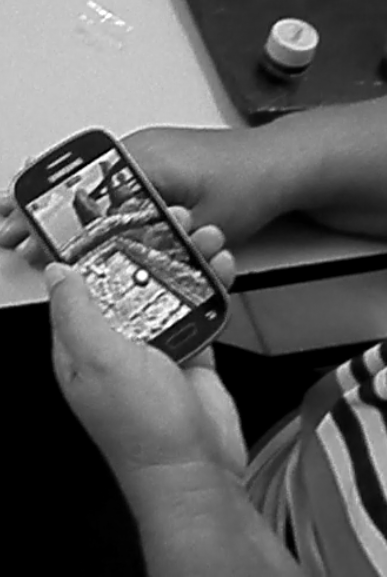
\includegraphics[scale=0.5]{./img/gametremor.png}
	% matrixargseg.png: 296x162 pixel, 100dpi, 7.52x4.11 cm, bb=0 0 213 117
	%\caption{Estágio desenvolvimento de jogos ~\cite{fullerton2008game}}
	\caption{Teste de um jogo usando acelerômetro para quantificação do sinal de tremor do Parkinson}
	%  \caption{Estágio desenvolvimento de jogos}
	\label{fig:gametremor}
	\end{figure}

\begin{itemize}
	\item O \textbf{REQ-ENTREVISTAS-01} não foi possível, pois o tremor de repouso é um dos principais sinais do~\ac{dp}. Sabíamos da sua importância, inclusive foi desenvolvido um jogo para \textit{Smartphone} que pudesse quantificar o tremor (Figura ~\ref{fig:gametremor}). Porém, no teste junto aos usuários, foi percebido que, no momento do uso, os pacientes com~\ac{dp} cessavam o tremor, inviabilizando assim sua quantificação. 
	\item O \textbf{[REQ-ENTREVISTAS-03]} não foi possível, pois a técnica de \textit{finger-tapping} não pode ser avaliadas utilizando o MS-Kinnect 1.0, uma vez que nessa versão não existe a captura do movimento dos dedos, conforme ilustrado na Figura~\ref{fig:articulacoeskinnect}.
	\item O \textbf{REQ-ENTREVISTAS-09} não foi possível, pois, por envolver estado emocional e parâmetros que não estamos levando em consideração nesse trabalho, esse requisito está fora do escopo. Entretanto, com mecanismos de detecção de batimentos cardíacos presente no MS-Kinnect 2.0, pode ser averiguada a relação dos batimentos cardíacos com o tremor.
\end{itemize}




%Em estudos prévios da nossa pesquisa, pudemos identificar esse fenômeno junto aos pacientes do~\ac{dp}, onde percebemos que os pacientes de~\ac{dp} cessavam o tremor quando confrontados com um jogo para celular desenvolvido com o propósito de quantificar o sinal do tremor (Figura~\ref{fig:gametremor}). Por esse motivo, resolvemos trabalhar com outro sinal do~\ac{dp} como a bradicinesia~\cite{protpar010} o qual pode ser avaliado utilizando um sensor de movimentos como o \textit{Ms-Kinnect Versão 1.0}~\cite{kinnect2013}. %que não necessita do contato físico do usuário além de ser utilizado em jogos eletrônicos. 



\subsubsection{Matriz de Rastreabilidade - Fragmento x Requisitos}
%\begin{center}
%\begin{table}[!htbp]
\begin{table}[!htb]
\caption{Matriz Rastreabilidade: Fragmento x Requisitos}
\label{table:matrix_rastreabilidade}
\begin{tabular}{||p{6.06cm}||ccccccccc|}
\hline
 \multicolumn{1}{|p{6.06cm}|}{\centering \textbf{FRAGMENTOS / REQUISITOS}} &  01 &  02 &  03 &  04 &  05 &  06 &  07 &  08 & 09 \\ 
\hline 
 \multicolumn{1}{|p{6.06cm}|}{\centering 01} &  x &  x &  x &  x &   &   &   &   &  \\ 
 \multicolumn{1}{|p{6.06cm}|}{\centering 02} &  x &   &   &   &   &  x &   &   &  \\ 
 \multicolumn{1}{|p{6.06cm}|}{\centering 03} &  x &  x &   &  x &  x &   &   &   &  \\ 
 \multicolumn{1}{|p{6.06cm}|}{\centering 04} &  x &   &   &   &   &   &   &   & x \\ 
 \multicolumn{1}{|p{6.06cm}|}{\centering 05} &  x &  x &   &   &   &   &   &   &  \\ 
 \multicolumn{1}{|p{6.06cm}|}{\centering 06} &   &  x &   &   &   &  x &   &   &  \\ 
 \multicolumn{1}{|p{6.06cm}|}{\centering 07} &   &  x &   &   &   &  x &  x &  x &  \\ 
 \multicolumn{1}{|p{6.06cm}|}{\centering 08} &   &  x &   &   &   &  x &  x &  x &  \\ 
 \multicolumn{1}{|p{6.06cm}|}{\centering 09} &   &   &   &  x &   &  x &   &   &  \\ 
 \multicolumn{1}{|p{6.06cm}|}{\centering 10} &   &   &   &   &   &  x &   &   &  \\ 
 \multicolumn{1}{|p{6.06cm}|}{\centering 11} &   &   &   &   &   &   &  x &   &  \\ 
 \multicolumn{1}{|p{6.06cm}|}{\centering 12} &   &  x &   &   &   &   &  x &  x &  \\ 
 \multicolumn{1}{|p{6.06cm}|}{\centering 13} &   &   &   &   &   &   &  x &   &  \\ 
 \multicolumn{1}{|p{6.06cm}|}{\centering 14} &   &  x &   &   &   &   &   &   &  \\ 
 \multicolumn{1}{|p{6.06cm}|}{\centering 15} &   &  x &   &  x &   &   &   &  x &  \\ 
 \multicolumn{1}{|p{6.06cm}|}{\centering 16} &   &   &   &  x &   &   &   &   &  \\ 
 \multicolumn{1}{|p{6.06cm}|}{\centering 17} &   &   &   &   &   &   &   &   &  \\ 
 \multicolumn{1}{|p{6.06cm}|}{\centering 18} &  x &   &  x &  x &   &  x &  x &  x & x \\ 
 \multicolumn{1}{|p{6.06cm}|}{\centering 19} &  x &   &   &   &  x &  x &  x &  x &  \\ 
 \multicolumn{1}{|p{6.06cm}|}{\centering 20} &  x &   &   &   &  x &  x &  x &  x &  \\ 
 \multicolumn{1}{|p{6.06cm}|}{\centering 21} &  x &   &   &   &  x &  x &  x &  x &  \\ 
\hline 
 \multicolumn{1}{|p{6.06cm}|}{\centering \textbf{QTD. OCORRÊNCIAS}} &  9 &  9 &  2 &  6 &  4 &  10 &  9 &  8 & 2 \\ 
\hline 
\end{tabular}
\end{table}

A Matriz de Rastreabilidade (Fragmento x Requisitos) mapeia os \textbf{REQUISITOS} aos \textbf{FRAGMENTOS} que, de forma direta ou indireta, estejam correlacionados (Tabela \ref{table:matrix_rastreabilidade}). Ao final, é obtido um campo de quantidade de ocorrências quantificando a sua ocorrência nos fragmentos.


%\end{center}

\subsubsection{Matriz de Rastreabilidade - Requisitos x Implementação}


A Matriz de Rastreabilidade (Tabela~\ref{table:RequisitoImplementado}) mapeia os \textbf{REQUISITOS} implementados neste trabalho e os que, devido a restrições técnicas, ainda estão em aberto. Isso demonstra também o estado atual do trabalho e pode direcionar os trabalhos futuros.

\begin{table}[!h]
\centering
\caption{Requisitos Implementados}
\label{table:RequisitoImplementado}
\begin{tabular}{|c|c|c|}
\hline
\textbf{REQUISITO} & \textbf{IMPLEMENTADO} & \textbf{INVIABILIDADE TÉCNICA}\\ \hline
REQ-ENTREVISTA-01                   &                                                             & X                                                                                                                \\ \hline
REQ-ENTREVISTA-02                   & X                                                           &                                                                                                                  \\ \hline
REQ-ENTREVISTA-03                   &                                                             & X                                                                                                                \\ \hline
REQ-ENTREVISTA-04                   & X                                                           &                                                                                                                  \\ \hline
REQ-ENTREVISTA-05                   & X                                                           &                                                                                                                  \\ \hline
REQ-ENTREVISTA-06                   & X                                                           &                                                                                                                  \\ \hline
REQ-ENTREVISTA-07                   & X                                                           &                                                                                                                  \\ \hline
REQ-ENTREVISTA-08                   & X                                                           &                                                                                                                  \\ \hline
REQ-ENTREVISTA-09                   &                                                             & X                                                                                                                \\ \hline
\end{tabular}
\end{table}
% Please remember to add \use{multirow} to your document preamble in order to suppor multirow cells
% Please remember to add \use{multirow} to your document preamble in order to suppor multirow cells




\subsection{Considerações Finais Sobre a Entrevisa SemiEstruturada}
O intuito dessa entrevista foi verificar, junto aos profissionais de saúde, os benefícios trazidos pelo monitoramento em relação à qualidade de vida e ao acompanhamento do tratamento do paciente.

Com base na rastreabilidade dos fragmentos da entrevista, pode-se concluir que existiram muitas ocorrências nos requisitos de identificação de sinais, tais como: tremores ([\textbf{REQ-ENTREVISTAS-01}]), bradicinesia [\textbf{REQ-ENTREVISTAS-02}] e análise da marcha [\textbf{REQ-ENTREVISTAS-06}]. Para o acompanhamento e o monitoramento da doença, os profissionais de saúde citaram a importância de calcular tanto a amplitude dos movimentos de abdução e adução dos braços ([\textbf{REQ-ENTREVISTAS-07}]), quanto a velocidade angular ([\textbf{REQ-ENTREVISTAS-08}]). Baseado nessas considerações, podemos validar qualitativamente a ETAPA 1 da pesquisa.


\section{ETAPA 2: Máquina de Vetor de Suporte para Estudo Analítico de Caso Controle Por Intermédio de Sensor de Movimento Usado em Jogos Eletrônicos}\label{sec:resultado_svm}

Partindo da importância de identificar o sintoma da bradicinesia e, consequentemente, avaliar a dificuldade do movimento (Seção ~\ref{section:analise_bradicinesia}), nessa pesquisa, buscou-se avaliar esse sintoma com o movimento de adução e abdução dos braços (ver Figura ~\ref{fig:movabducaomet}). A abordagem de aprendizagem de máquina foi utilizada para classificar portadores do~\ac{dp} ante indivíduos sem o diagnóstico. Partiu-se do princípio que os indivíduos com~\ac{dp} teriam mais dificuldade ao levantar o braço, e a sua velocidade angular seria reduzida ante os indivíduos que não desenvolveram a doença.

\subsection{Estudo analítico de caso-controle}\label{section:estudo_caso_controle}
Esta etapa da pesquisa foi pautada pelo protocolo de pesquisa avaliado pelo Comitê de Ética da UFCG (Apêndice~\ref{sec:comite}). Somente após a aprovação deste (\textbf{CAAE: 14408213.9.1001.5182}), é que os dados foram coletados. 

O resultado alcançado com esse estudo análitico de caso-controle foi identificar mecanismos de classificação de pessoas saudáveis ante pacientes com~\ac{dp}. Durante a pesquisa, analisamos o sensor de movimento MS-Kinnect~\cite{kinnect2013} para avaliar a possibilidade de aquisição de dados de saúde, baseada na Cinemática Linear do Movimento Humano~\cite{mcginnis2013biomechanics}. A partir dos resultados obtidos, pudemos avaliar a normalidade e a dificuldade na execução de movimentos, como, por exemplo, levantar um braço~\cite{mcginnis2013biomechanics}.

A coleta de dados dos pacientes com~\ac{dp} foi realizada no Hospital Universitário da UFAL e na Fundação Pestalozzi em Maceió, sob a a tutela da Profa. e Neurologista Dra. Cícera Pontes; e a do grupo controle, na Clínica de Fisioterapia do CESMAC, sob a tutela do Prof. de Fisioterapia Jean Charles Santos. As coletas foram realizadas em local reservado e de forma individual, com a anuência do sujeito pesquisado através da assinatura do Termo de Consentimento.

\subsubsection{Amostra}
Foram selecionados, por disponibilidade, um total de 30 sujeitos da pesquisa. O grupo previamente diagnosticado por neurologistas com~\ac{dp} consistiu de 15 indivíduos; destes, 10 eram homens e 5 mulheres, entre 51 e 65 anos (média : 58 anos). O grupo controle foi composto por 15 indivíduos sem diagnóstico com~\ac{dp}; destes, 11 eram homens e 4 mulheres, entre 50 e 65 anos (média : 57 anos). Todos os indivíduos fizeram uso da abordagem de monitoramento baseada em jogos proposta neste trabalho. Os sujeitos da pesquisa foram solicitados a executarem os movimentos de abdução e adução dos braços de acordo com a proposta do jogo. Todas as sessões foram realizadas sob supervisão de um neurologista ou fisioterapeuta, quando foi verificado o estado de saúde dos sujeitos da pesquisa. 


\subsubsection{Recrutamento dos Sujeitos e Aquisição do Consentimento Livre e Esclarecido}
O recrutamento deste protocolo estava circunscrito por intermédio de um profissional de saúde. O profissional conhecia a história clínica do paciente e obteve a sua permissão. No momento da coleta, a equipe de pesquisa explicitou os riscos e os benefícios na participação da pesquisa e buscou a arbitrariedade e a espontaneidade da decisão. Depois, foi oferecido, para assinatura, o Termo de Consentimento Livre e Esclarecido.

\subsubsection{Critérios de Inclusão}
Foram inclusos na pesquisa os indivíduos do grupo diagnosticados com~\ac{dp} no estágio 3, segundo a UPDRS~\cite{updrs87}, sem distinção de gênero ou cor. Os indivíduos ficaram dentro das facilidades da clínica onde a coleta foi realizada e aceitaram participar do estudo. O grupo de indivíduos que não estavam diagnosticados com~\ac{dp} informaram que nunca receberam o diagnóstico da doença e aceitariam participar do estudo como grupo controle.

\subsubsection{Critérios de Exclusão}
Foram excluídos das pesquisas os indivíduos com problemas de equilíbrio ou questionamento de dores ao executar os procedimentos. Foram excluídos também os indivíduos que por qualquer motivo se negaram a participar do estudo.

\subsubsection{Materiais}
Para a presente pesquisa foram coletados movimentos de abdução e adução dos braços~\cite{mcginnis2013biomechanics}, que podem ser incorporados a um jogo eletrônico. Foi utilizado um jogo com o arcabouço de software de captura de dados (~\ac{jogue-me}). 

Durante a execução da coleta, houve uma preocupação com a integridade física dos participantes. Então, os movimentos utilizados no jogo foram apenas de adução e abdução dos braços~\cite{mcginnis2013biomechanics}, o que proporcionou a devida segurança aos participantes. 

% \subsubsection{Infra-Estrutura}
% A pesquisa foi realizada na clínica onde o paciente estava em tratamento. O espaço físico forneceu condições favoráveis e adequadas para a aplicação da coleta. Para a realização da pesquisa foram utilizados os seguintes instrumentos:
% 
% \begin{itemize}
% 	\item O Jogo \textit{Catch the Spheres}, rodando em notebook com Sistema Operacional Windows 7.0 e Unity 3d 3.0;
% 	\item O Projetor (Epson Lcd Powerlite X14 3000l Hdmi), para projetar o jogo na parede e facilitar a visualização;
% 	\item O Sensor de movimento Ms-Kinnect 1.0~\cite{kinnect2013}.
% \end{itemize}

\subsubsection{Métodos}
Nesta pesquisa, foi realizada uma análise de um sensor de movimento utilizado em jogos eletrônicos e avaliada a possibilidade de aquisição de dados de saúde baseada na Cinemática Angular do Movimento Humano~\cite{hamill1999bases}.  Através dos resultados obtidos, conseguimos classificar a normalidade e a dificuldade na execução de movimentos como abdução e adução dos braços.

A coleta de dados foi realizada no próprio espaço de tratamento do indivíduo, em local reservado e de forma individual. A participação do indivíduo foi consentida por meio da assinatura do Termo de Consentimento. Devido às restrições de tempo (1 minuto e 30 segundos) e da execução de um mesmo movimento por todos os participantes, foram solicitados dos voluntários a execução dos seguintes procedimentos:
\begin{enumerate}
	\item O voluntário se posiciona a uma distância de 2 metros do sensor de movimento, de modo a conseguir capturar toda a extensão superior do braço durante o movimento de abdução; 	
	\item O voluntário inicia o jogo \textit{Catch the Spheres} usando a mão esquerda conforme a interface da aplicação;
	\item O voluntário abduz e aduz 10 vezes o braço esquerdo e depois o braço direito o mais amplo e o mais rápido possível, de modo a permitir que fossem adquiridas a amplitude de movimento e a velocidade angular. 
	\item O voluntário fecha a aplicação, e esta realiza o armazenamento e envio dos dados ao servidor.
\end{enumerate}

\begin{figure}[!htbp]
 \centering
 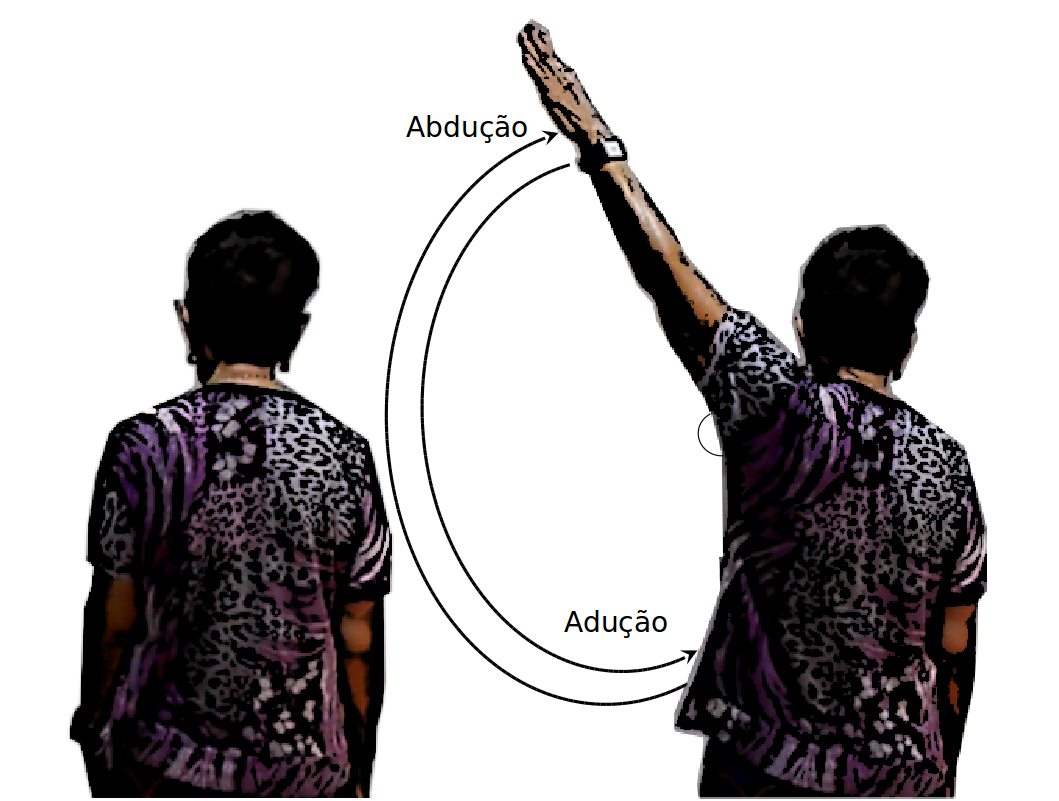
\includegraphics[scale=0.25]{./img/movaddcutctionartist2.png}
 % matrixargseg.png: 296x162 pixel, 100dpi, 7.52x4.11 cm, bb=0 0 213 117
 %\caption{Estágio desenvolvimento de jogos ~\cite{fullerton2008game}}
\caption{Movimentos de Abdução e Adução}
%  \caption{Estágio desenvolvimento de jogos}
 \label{fig:movabducaomet}
\end{figure}

Durante a análise, foram comparados os Ângulos Relativos do Tronco e do Levantamento de Braços dos Indivíduos. As grandezas cinemáticas coletadas nesses estudo foram:
\begin{enumerate}
	\item A máxima amplitude atingida pelo movimento de abdução dos membros superiores;
	\item A velocidade angular de abdução dos membros superiores esquerdo e direito;
	\item A velocidade angular de adução dos membros superiores esquerdo e direito.
\end{enumerate}

Os dados coletados nesta fase resultaram na extração de características do movimento, incluindo: a amplitude do movimento dos braços do lado esquerdo e direito, e a velocidade angular dos movimentos de adução e abdução. Na Tabela~\ref{table:features} estão descritos os vetores de características:
\begin{table}[h]
\centering
\caption{Descrição do vetor de características extraído da coleta de dados.}
\label{table:features}
\begin{tabular}{|l|l|}
\hline
{\bf Característica}  & {\bf Descrição}                                       \\ \hline
MaxAmpEsquerdo     & Amplitude máxima do braço esquerdo. \\ \hline
MaxAmpDireito    & Amplitude máxima do braço direito. \\ \hline
AngVelAbdEsquerdo  & Velocidade angular do movimento de abdução do braço esquerdo. \\ \hline
AngVelAbdDireito & Velocidade angular do movimento de abdução do braço direito. \\ \hline
AngVelAdEsquerdo  & Velocidade angular do movimento de adução do braço esquerdo. \\ \hline
AngVelAdDireito & Velocidade angular do movimento de adução do braço direito. \\ \hline
\end{tabular}
\end{table}

\begin{figure}[!htb]
	\centering
	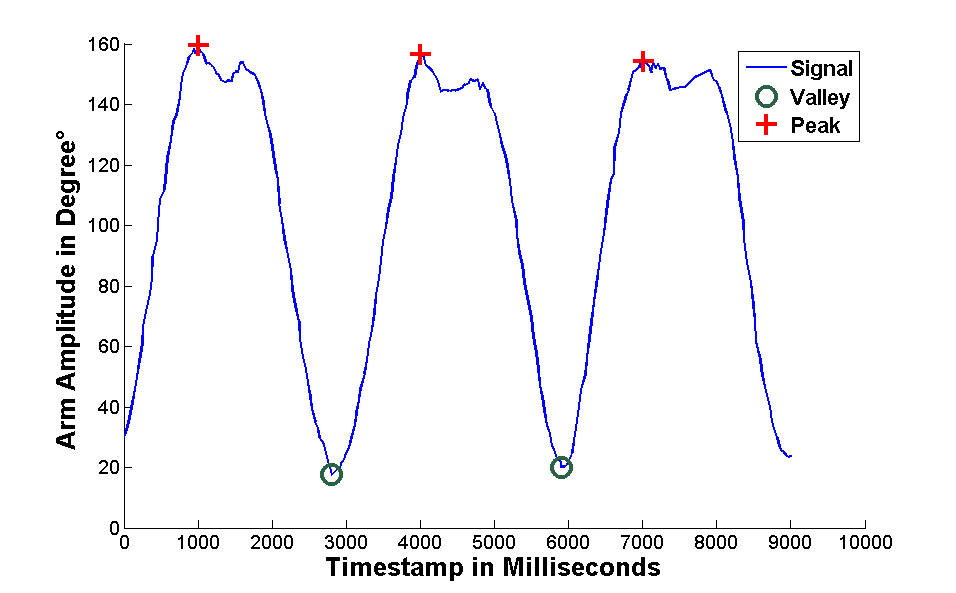
\includegraphics[width=1\textwidth]{img/signalamplitudepeakvaley-2.png}
	\caption{Exemplo do gráfico dos ângulos de adução e abdução dos braços em função do tempo}
	\label{fig:signalamplitudepeakvaley}
\end{figure}

A partir da extração das características do movimento, a próxima etapa da pesquisa foi classificar os dados de movimento e identificar a ocorrência do sintoma de bradicinesia. Por meio das teorias estatísticas de aprendizagem de máquina, foi realizado uma análise dos dados para aquisição de conhecimento utilizando aprendizagem supervisionada~\cite{kantardzic2011data}. 


\subsubsection{Relação Risco e Benefício da Pesquisa}
Os riscos inerentes podem decorrer da exposição de dados dos sujeitos da pesquisa. Isso pode acarretar em danos morais e/ou psicológicos. Logo, teve-se um cuidado de preservar a integridade física e psicológica dos sujeitos da pesquisa, garantindo assim a privacidade e a confidencialidade das informações.

Caso ocorresse algum constrangimento por parte do sujeito da pesquisa, ao não conseguir realizá-la, os pesquisadores prestariam total assistência, orientando-o adequadamente para prosseguir ou encerrar o procedimento. Os presentes riscos fazem jus aos benefícios que a pesquisa venha a trazer com a possibilidade de monitoramento dos sinais do~\ac{dp}. A identificação dos sinais motores e a classificação destes através do computador podem permitir avanços para um melhor acompanhamento da evolução da doença e possibilitar o monitoramento não invasivo dos pacientes.



\subsection{Aplicação do Método}
O propósito dessa classificação foi explorar a possibilidade de obter dados de saúde de forma contínua e não invasiva a partir de um sensor de captura de movimento usado em jogos eletrônicos (Ms-Kinnect). Durante a coleta dos dados foi indagado junto aos voluntários sua condição física e possíveis riscos e desconfortos que eles pudessem ter ao realizar o procedimento. 

Durante a pesquisa, partiu-se do princípio de que, através da análise do movimento de abdução e adução dos braços seria possível avaliar a biomecânica da amplitude do movimento dos braços e a sua velocidade angular. Então, por intermédio desses dados biomecânicos, seria possível identificar a ocorrência do sintoma de bradicinesia em indivíduos portadores do \ac{dp}.



\subsection{Resultados}
Conforme a abordagem~\ac{jogue-me} apresentada no Capítulo~\ref{chapter:abordagem_gahme}, os dados adquiridos foram processados, filtrados e postos em uma Máquina de Vetor de Suporte, para realizar a classificação entra as duas classes de dados. Para a classificação dos dados, foi utilizado um \textit{kernel} Linear (Seção~\ref{sec:svm_linear}), por ter obtido os melhores resultados dentre os demais \textit{kernels} (Polinomial, Radial e de MLP). O resultado do \textit{kernel} linear foi o mais expressivo entre os demais devido à separação linear ter dividido bem as duas classes. 

\subsubsection{Vetor Médio}
Nessa etapa da pesquisa, foi calculado o Vetor Médio (Seção~\ref{section:filtro_dados}), para entender melhor a diferença de movimento entre os sujeitos diagnosticados com \ac{dp} e os sujeitos sem o diagnóstico. Como pode ser visto na Figura~\ref{fig:vetor_medio_abducao}, a amplitude de movimento de um indivíduo diagnosticado com~\ac{dp} é bem menor do que a de um indivíduo sem o diagnóstico. Entretanto, por ter sido escalonado em 20 \textit{frames}, esse vetor médio perdeu a informação da velocidade do movimento.

\begin{figure}[!htbp]
 \centering
 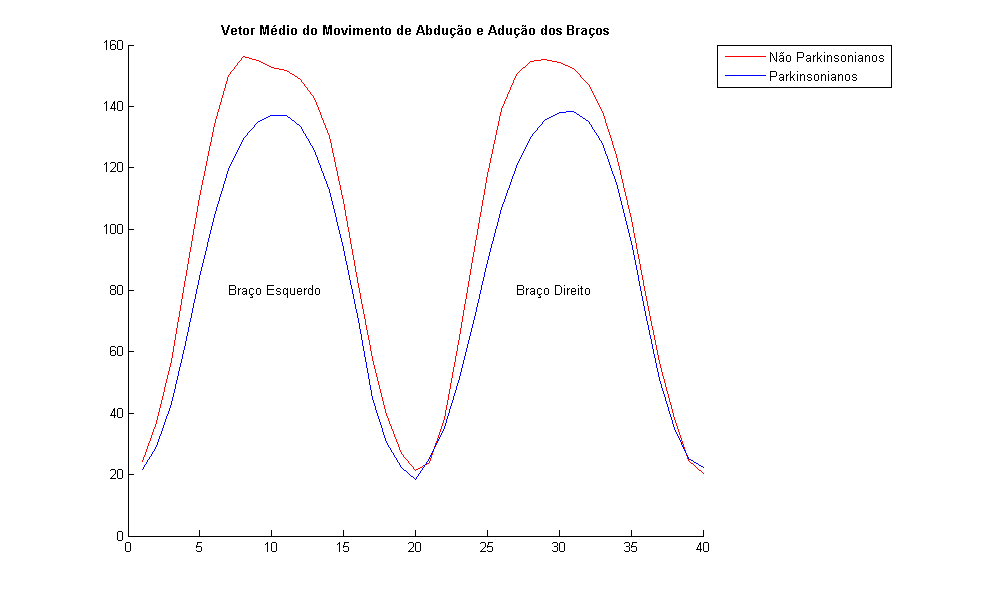
\includegraphics[scale=0.650]{./img/vetormedioaducao.png}
 \caption{Vetor Médio do Movimento de Abdução e Adução}
 \label{fig:vetor_medio_abducao}
\end{figure}


\subsubsection{Matriz de Confusão e Suas Métricas}
Para avaliar o resultado da classificação, será apresentada a \textbf{matriz de confusão}~\cite{kantardzic2011data}, que permite comparar os valores reais da classe com os valores obtidos no modelo de predição. 

A matriz de confusão para duas classes consiste numa matriz $2$\ x $2$\, contendo os \textit{Verdadeiros Positivos} (\textbf{TP}) e \textit{Verdadeiros Negativos} (\textbf{TN}), que são as classificações corretas. Os \textit{Falsos Negativos} (\textbf{FN}) contêm a predição incorreta de um valor que deveria ser positivo e os \textit{Falsos Positivos} (\textbf{FP}) contêm os valores positivos quando deveriam ser negativos, como pode ser visto na Tabela~\ref{table:descricaomatrizconfusao}.

% Please remember to add \use{multirow} to your document preamble in order to suppor multirow cells
\begin{table}[!htbp]
\caption{Descrição da Matriz de Confusão}
\label{table:descricaomatrizconfusao}
\begin{tabular}{ll|c|c|}
\cline{3-4}
                                                                                                               & \multicolumn{1}{c}{}                         & \multicolumn{2}{|c|}{\textit{\textbf{Classe Preditiva}}} \\ \cline{3-4} 
                                                                                                               &                                              & \textbf{Parkinson}          & \textbf{Controle}     \\ \hline
\multicolumn{1}{|c}{\multirow{\textit{\textbf{\begin{tabular}[c]{@{}c@{}}Classe\\ Atual\end{tabular}}}}} & \multicolumn{1}{|l|}{\textbf{Parkinson}}     & Verdadeiros Positivos (VP)  & Falsos Negativos (FN)      \\ \cline{2-4} 
\multicolumn{1}{|l}{\textit{\textbf{}}}                                                                        & \multicolumn{1}{|l|}{\textbf{Controle}} & Falsos Positivo (FP) & Verdadeiros Negativos (VN) \\ \hline
\end{tabular}
\end{table}




\subsection{Aprendizagem de Máquina (SVM)}

Para uma base de dados pequena, contendo apenas 30 indivíduos, o método de Validação Cruzada escolhido deve tentar maximizar o conjunto de treinamento para atingir um melhor resultado de teste. Por esse motivo, foi escolhida a validação cruzada \textit{leave-one-out}~\cite{kantardzic2011data}. 

O \textit{leave-one-out} é um método de validação cruzada \textit{k-fold} com o mesmo número de \textit{n} indivíduos. Logo, apenas um indivíduo será considerado teste e os demais serão de treinamento. Dessa maneira, não existe estratificação nos dados, tornando o processo determinístico e repetível com a mesma base de dados, o que reduz o problema de viés na seleção dos dados. Logo, a taxa de erro obtida da classificação é a taxa de erro do modelo para aquela base de dados. 

\subsubsection{Otimização dos Parâmetros da SVM - Método Grid-Search}

Para identificar os melhores parâmetros~\ac{svm}, foi aplicado o método~\textit{Grid-Search} ~\cite{gridsearchsvm2010} usando validação cruzada \textit{Leave-One-Out} (LOOCV)~\cite{kantardzic2011data}. Este método avalia a precisão do modelo previsto, evita o problema do superajuste na classificação binária e é um método prático para identificar os parâmetros SVM . Neste estudo, para reduzir a taxa de erro, nós aplicamos uma abordagem de \textit{minimax} visando maximizar a margem sobre os coeficientes hiperplano para obter uma classificação mais correta. Os valores dos parâmetros de pesquisa do \textit{grid-search} foram de: $C$ = [$2^5$, ... ,$2^2$] e $\gamma$ = [$2^{15}$, ... ,$2^3$ ], usando assim uma exponencial de base 2. Por meio deste método, foi possível identificar uma região em que o classificador possuía a melhor acurácia e a menor taxa de \textit{FpRate}. Após identificar essa região, realizamos uma busca mais detalhada com os seguintes parâmetros: $C$ = [0.25, 0.5, ... ,2.5]; e $\gamma$ = [1, 2,
 ...,10], como pode ser visto na Figura~\ref{fig:gridaccuracy}.


\begin{figure}[!h]
 \centering
  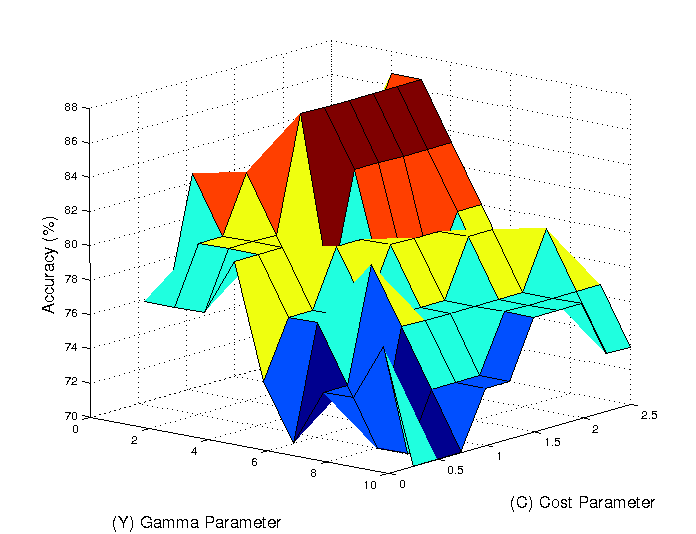
\includegraphics[scale=0.7]{./img/gridsearch.png} 
  \caption{\textit{Grid-Search} - Acurácia da Classificação}
 \label{fig:gridaccuracy}
\end{figure}

 
Como pode ser analisado na Figura~\ref{fig:gridaccuracy}, nós conseguimos uma classificação nos dados em que a pior predição obteve uma acurácia de 70,00\% e a melhor, de 86,67\%. Conseguimos também um baixo valor de \textit{FpRate}, com 6,67\% no melhor dos casos (Figura~\ref{fig:gridfprate}). Usando o método \textit{grid-search}, nós encontramos como melhor valor para os parâmetros: $C = 2$ and $\gamma = 3$. Como podemos analisar nos nossos resultados, por meio do método \textit{grid-search}, foi possível identificar parâmetros para o classificador~\ac{svm} com uma boa generalização e capaz de identificar a maior \textit{acurácia} e o menor \textit{FpRate}.


\begin{figure}[!h]
 \centering
 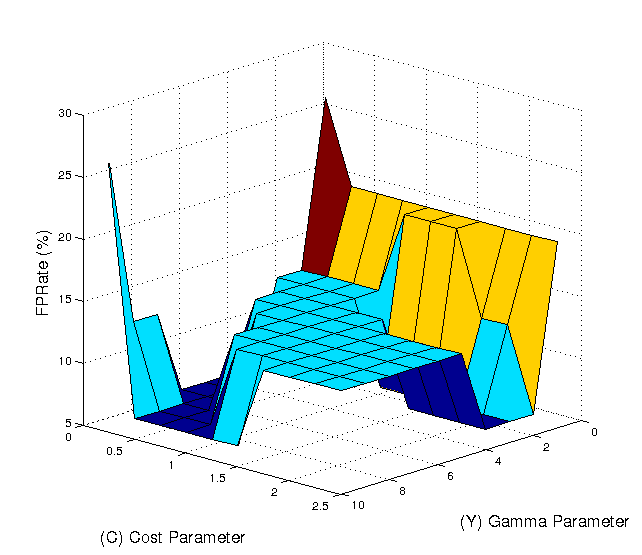
\includegraphics[scale=0.7]{./img/gridsearchfprate.png}
 % matrixargseg.png: 296x162 pixel, 100dpi, 7.52x4.11 cm, bb=0 0 213 117
 %\caption{Estágio desenvolvimento de jogos ~\cite{fullerton2008game}}
\caption{\textit{Grid-Search} - \textit{FpRate}}
%  \caption{Estágio desenvolvimento de jogos}
 \label{fig:gridfprate}
\end{figure}


\subsubsection{Resultados Obtidos}\label{sec:resultado_obtido_svm}


A Matriz de Confusão obtida indica que existem três indivíduos classificados como ``Controle'', mas que possuem a doença (FN); no entanto, analisando as características do movimento dos indivíduos com~\ac{dp}, percebemos que eles apresentaram uma amplitude de movimento e uma velocidade angular bastante próximas dos indivíduos do Grupo Controle. Logo, estes não apresentam o sintoma de bradicinesia, o que pode indicar que o indivíduo esteja no início da doença, ou bem medicado, ou até mesmo não apresentar este sinal motor, o que corrobora com a sintomatologia do~\ac{dp}. 
%Um resultado, que não era esperado nesta pesquisa é a ocorrência de um indivíduo que não possui~\ac{dp} mas mesmo assim foi classificados com o sintoma. Analisando seus dados foi percebido que ele possuía sinais muito próximos do grupo dos indivíduos com~\ac{dp}, logo ele possivelmente apresenta algum déficit motor o que condiz com o resultado da classificação.

\begin{table}[!htbp] 
\caption{Resultado da Matriz de Confusão SVM}
\label{table:resultadomatrizconfusaosvm}
\centering
\begin{tabular}{l|c|c|}
\cline{2-3}
\multicolumn{1}{c}{}                         & \multicolumn{2}{|c|}{\textit{\textbf{Classe Preditiva}}} \\ \cline{2-3} 
                                             & \textbf{Parkinson}      & \textbf{Controle}         \\ \hline
\multicolumn{1}{|l|}{\textbf{Parkinson}} & 12       & 3           \\ \hline
\multicolumn{1}{|l|}{\textbf{Controle}}     & 1           & 14     \\ \hline
\end{tabular}

\end{table}

O sinal da bradicinesia presente no~\ac{dp} foi quantificado pela amplitude do movimento de abdução dos braços e sua respectiva velocidade angular. Na análise destes sinais, foi possível extrair os vetores de características para a classificação dos dados~\cite{kantardzic2011data}. Na Tabela~\ref{table:amplitude}, podemos demonstrar a severidade do sinal motor causado pela bradicinesia, em que o Grupo com~\ac{dp} apresentou amplitudes bem menores ante os indivíduos do Grupo Controle. Notamos também que o indivíduo ``Controle 10'' apresentou uma amplitude muito semelhante aos do Grupo com~\ac{dp}. Neste caso, nós identificamos que ele apresentava um problema motor e isso ocasionou uma classificação incorreta por parte da~\ac{svm}. Além disso, 3 indivíduos do Grupo com~\ac{dp} (3,8 e 12) não apresentavam o sinal da bradicinesia durante a coleta. Nestes casos, podemos assumir que eles não possuem a bradicinesia, ou o sinal estava suprimido pela medicação.


\begin{table}[!htp]
\centering
\caption{Média da Amplitude do Movimento de Abdução do Braço}
\label{table:amplitude}
\begin{tabular}{|l|l|l|l|}
\hline
\textbf{Indivíduo} & \textbf{\begin{tabular}[c]{@{}l@{}}Média da\\ Amplitude \\ Braço Esquerdo(º)\end{tabular}} & \textbf{\begin{tabular}[c]{@{}l@{}}Média da\\ Amplitude\\ Braço Direito(º) \end{tabular}} & \textbf{\begin{tabular}[c]{@{}l@{}}Classe\\ Preditiva\end{tabular}} \\ \hline
Controle 1         & \multicolumn{1}{r|}{153.62}                                                          & \multicolumn{1}{r|}{151.14}                                                          & Controle                                                            \\ \hline
Controle 2         & \multicolumn{1}{r|}{165.31}                                                          & \multicolumn{1}{r|}{151.84}                                                          & Controle                                                            \\ \hline
Controle 3         & \multicolumn{1}{r|}{155.44}                                                          & \multicolumn{1}{r|}{163.31}                                                          & Controle                                                            \\ \hline
Controle 4         & \multicolumn{1}{r|}{169.12}                                                          & \multicolumn{1}{r|}{169.39}                                                          & Controle                                                            \\ \hline
Controle 5         & \multicolumn{1}{r|}{157.20}                                                          & \multicolumn{1}{r|}{162.72}                                                          & Controle                                                            \\ \hline
Controle 6         & \multicolumn{1}{r|}{162.99}                                                          & \multicolumn{1}{r|}{167.25}                                                          & Controle                                                            \\ \hline
Controle 7         & \multicolumn{1}{r|}{166.90}                                                          & \multicolumn{1}{r|}{166.93}                                                          & Controle                                                            \\ \hline
Controle 8         & \multicolumn{1}{r|}{154.68}                                                          & \multicolumn{1}{r|}{159.13}                                                          & Controle                                                            \\ \hline
Controle 9         & \multicolumn{1}{r|}{162.31}                                                          & \multicolumn{1}{r|}{158.17}                                                          & Controle                                                            \\ \hline
Controle 10         & \multicolumn{1}{r|}{135.22}                                                          & \multicolumn{1}{r|}{131.85}                                                          & \textbf{Parkinson}                                                            \\ \hline
Controle 11         & \multicolumn{1}{r|}{162.13}                                                          & \multicolumn{1}{r|}{167.61}                                                          & Controle                                                            \\ \hline
Controle 12         & \multicolumn{1}{r|}{161.69}                                                          & \multicolumn{1}{r|}{166.78}                                                          & Controle                                                            \\ \hline
Controle 13         & \multicolumn{1}{r|}{160.47}                                                          & \multicolumn{1}{r|}{155.05}                                                          & Controle                                                            \\ \hline
Controle 14         & \multicolumn{1}{r|}{174.37}                                                          & \multicolumn{1}{r|}{167.66}                                                          & Controle                                                            \\ \hline
Controle 15         & \multicolumn{1}{r|}{155.08}                                                          & \multicolumn{1}{r|}{167.83}                                                          & Controle                                                            \\ \hline
Parkinson 1         & \multicolumn{1}{r|}{125.80}                                                          & \multicolumn{1}{r|}{119.73}                                                          & Parkinson                                                            \\ \hline
Parkinson 2         & \multicolumn{1}{r|}{131.28}                                                          & \multicolumn{1}{r|}{123.49}                                                          & Parkinson                                                            \\ \hline
Parkinson 3         & \multicolumn{1}{r|}{156.66}                                                          & \multicolumn{1}{r|}{149.46}                                                          & \textbf{Controle}                                                            \\ \hline
Parkinson 4         & \multicolumn{1}{r|}{139.90}                                                          & \multicolumn{1}{r|}{142.83}                                                          & Parkinson                                                            \\ \hline
Parkinson 5         & \multicolumn{1}{r|}{147.37}                                                          & \multicolumn{1}{r|}{153.13}                                                          & Parkinson         \\ \hline
Parkinson 6         & \multicolumn{1}{r|}{115.32}                                                          & \multicolumn{1}{r|}{123.56}                                                          & Parkinson                                                            \\ \hline
Parkinson 7         & \multicolumn{1}{r|}{129.75}                                                          & \multicolumn{1}{r|}{133.04}                                                          & Parkinson                                                            \\ \hline
Parkinson 8         & \multicolumn{1}{r|}{166.62}                                                          & \multicolumn{1}{r|}{165.63}                                                          & \textbf{Controle}                                                            \\ \hline
Parkinson 9         & \multicolumn{1}{r|}{143.95}                                                          & \multicolumn{1}{r|}{140.45}                                                          & Parkinson                                                            \\ \hline
Parkinson 10         & \multicolumn{1}{r|}{136.86}                                                          & \multicolumn{1}{r|}{151.03}                                                          & Parkinson                                                            \\ \hline
Parkinson 11         & \multicolumn{1}{r|}{156.87}                                                          & \multicolumn{1}{r|}{142.93}                                                          & Parkinson                                                            \\ \hline
Parkinson 12         & \multicolumn{1}{r|}{166.59}                                                          & \multicolumn{1}{r|}{157.81}                                                          & \textbf{Controle}                                                            \\ \hline
Parkinson 13         & \multicolumn{1}{r|}{147.99}                                                          & \multicolumn{1}{r|}{142.02}                                                          & Parkinson                                                            \\ \hline
Parkinson 14         & \multicolumn{1}{r|}{141.95}                                                          & \multicolumn{1}{r|}{150.60}                                                          & Parkinson                                                            \\ \hline
Parkinson 15         & \multicolumn{1}{r|}{125.69}                                                          & \multicolumn{1}{r|}{140.62}                                                          & Parkinson                                                            
\\ \hline
\end{tabular}
\end{table}

Para demonstrar a avaliação do modelo de forma quantitativa, usou-se um conjunto de métricas derivadas da matriz de confusão~\cite{kantardzic2011data}.
 \begin{description}
 	\item [\textit{TpRate}] taxa de acerto obtido: $ TpRate = TP/P $\ ;
 	\item [\textit{FpRate}]: taxa de falso alarme obtido: $ FpRate = FP/N $\ ;
 	\item [\textit{Precision}]: taxa de acerto de uma instância em determinada classe: $ Precision =  TP/(TP +FP) $\ ;
 	\item [\textit{Accuracy}]: taxa de acerto de todo o classificador: $ Accuracy = (TP+TN)/(P+N) $\ ;
 	\item [\textit{F-Measure}]: análise de classificador binário que mede a acurácia do teste, considerando a média harmônica da taxa de \textit{precision} e do \textit{tp rate}: $ F-Measure = 2 * (Precision * TpRate)/(Precision + TpRate) $\ .
 \end{description}



\begin{table}[!htbp]
\label{table:metricasmatrizconfusao}
\caption{Métricas da Matriz de Confusão}
\centering
\begin{tabular}{|l|r|}





\hline
\multicolumn{2}{|l|}{\textbf{Métricas}} \\ \hline
\textbf{TpRate}                    & 80,00$\%$\                 \\ \hline
\textbf{FpRate}                    & 6,67$\%$\                \\ \hline
\textbf{Precision}                 & 92,31$\%$\                \\ \hline
\textbf{Accuracy}                  & 86,67$\%$\                \\ \hline
\textbf{F-Measure}                 & 85,71$\%$\                \\ \hline
\end{tabular}
\end{table}








\section{ETAPA 3 - Avaliação Da Aceitação Da Abordagem Junto aos Pacientes com~\ac{dp} Utilizando \textit{Goal Question Metric}}\label{gqm_usuarios}


Com o objetivo de averiguar a possibilidade de integrar o monitoramento da saúde do jogador através de jogos eletrônicos à sua rotina diária, foi utilizada a abordagem \textit{Goal, Question, Metric} (GQM)~\cite{van1999goal}. Essa abordagem é um paradigma de pesquisa utilizado na Engenharia de Software para medição de processos de software e melhoria contínua dos produtos ~\cite{saraiva2006,elicquest05}. A qualidade do produto de software~\cite{saraiva2006} pode ser compreendida como a adequação a um conjunto de características atingidas em maior ou menor grau para que o produto final venha atender as necessidades do usuário, identificadas na fase de elicitação de requisitos~\cite{elicquest05}.

O~\ac{gqm} é um paradigma de avaliação orientado por metas e tem como componentes elementares: objetivos, questionamentos e métricas~\cite{saraiva2006}. Nesse paradigma de pesquisa é definido um objetivo principal, em que as perguntas são refinadas para que se venha extrair as métricas da pesquisa. De posse das respostas baseadas em métricas, estas são comparadas com o objetivo da pesquisa no intuito de identificar se ele foi alcançado. Logo, o paradigma~\ac{gqm} busca definir métricas partindo de uma perspectiva de ``de cima para baixo'', e analisa, interpreta e mensura dados de maneira ``de baixo para cima'', como pode ser graficamente visualizado na Figura~\ref{fig:gqm} ~\cite{van1999goal}. 

\begin{figure}[!htbp]
 \centering
 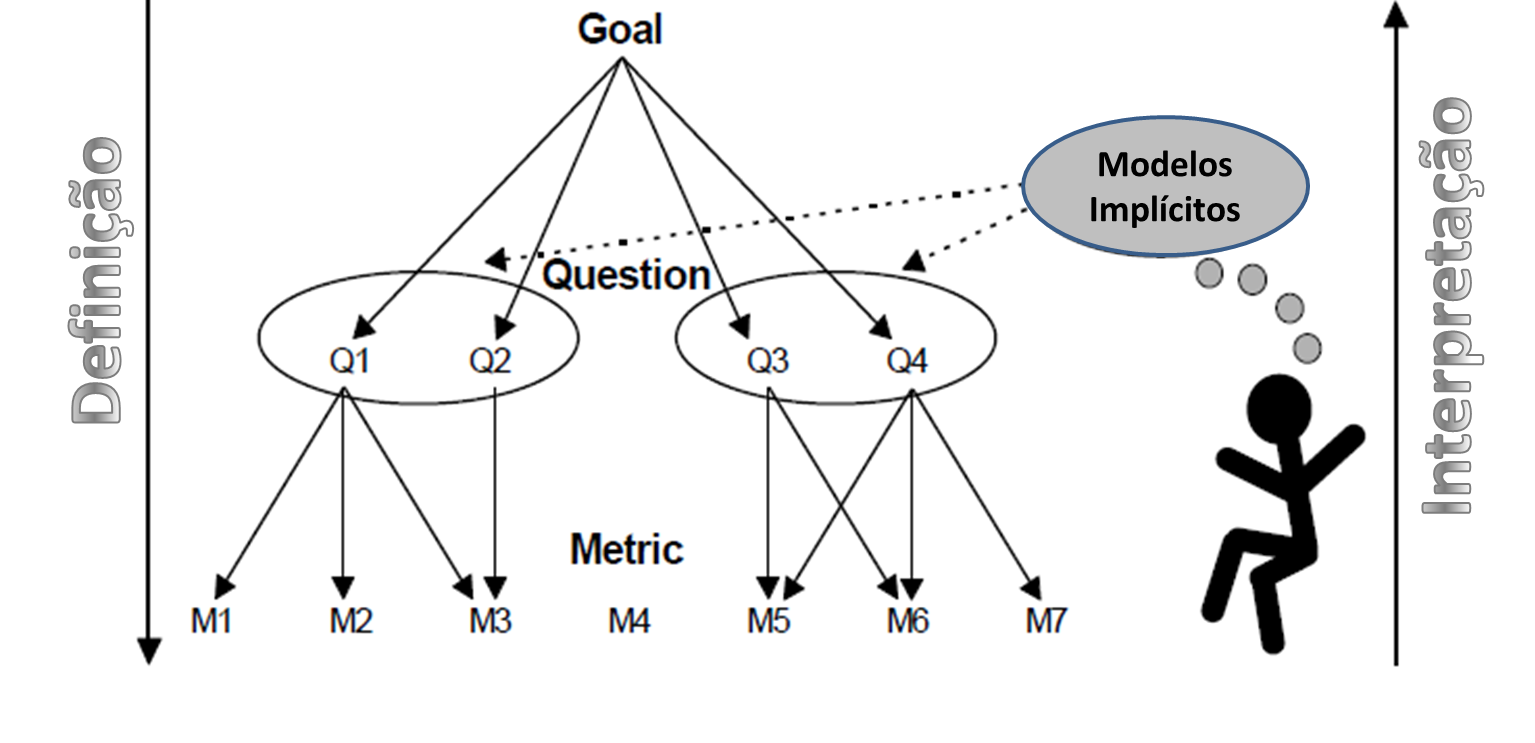
\includegraphics[scale=0.50]{./img/gqm.png}
 \caption[O Paradigma GQM \copyright]{O Paradigma GQM \copyright~\cite{van1999goal}}
 \label{fig:gqm}
\end{figure}

Segundo Saraiva ~\cite{saraiva2006}, numa análise da aplicação do método de ~\ac{gqm} para o contexto de avaliação de usabilidade de software, os componentes elementares do paradigma ~\ac{gqm} são:

\begin{itemize}
	\item \textbf{Objetivo}: Sua definição envolve o propósito da avaliação, o que deve ser avaliado, a perspectiva e o ambiente proposto.
	\item \textbf{Questão}: A questão anuncia a necessidade de se obter informações em linguagem natural, podendo formular uma ou mais questões para cada categoria. Logo, sua resposta deve estar condicionada ao objetivo proposto.
	\item \textbf{Métrica}: Sua função é especificar os dados que se deseja obter durante as avaliações em termos quantitativos, podendo ter mais de uma métrica para cada questão.	
\end{itemize}

Baseado nos componentes elementares do paradigma, foi elaborado um questionário~\ac{gqm} (Apêndice~\ref{apend:gqm}), com o objetivo principal de avaliar a possibilidade de monitorar dados motores, de forma não invasiva e integrada à rotina diária dos usuários. Para elaboração de métricas para atingir esse objetivo foram formuladas duas questões de pesquisa, com o intuito de avaliar:
\begin{enumerate}
	\item se o usuário integraria a abordagem~\ac{jogue-me} à sua rotina diária;
	\item se a segurança com a integridade física está de acordo com a faixa etária do usuário.
\end{enumerate}

O questionário consistiu de um conjunto de 10 questões de resposta fechada (quantitativa) ~\cite{elicquest05}, e o entrevistado teve de escolher uma resposta dentre as alternativas dadas. Esse método foi escolhido para contribuir por uma maior uniformidade nas respostas e, consequentemente, facilitar sua análise. Porém, este método impede a expressão das opiniões dos entrevistados~\cite{elicquest05}. 


\subsection{Aplicação do Método}
Nessa etapa da pesquisa foram avaliados 30 sujeitos, dos seguintes locais: Hospital Universitário da UFAL, Fundação Pestalozzi e clínica de Fisioterapia do CESMAC. Os usuários foram selecionados para jogar o \emph{Catch the Spheres} (Seção ~\ref{jogo_catch}), testaram e responderam o questionário para verificar a aceitabilidade da abordagem. 


\subsection{Resultados}
Os resultados do questionário são apresentados na Tabela~\ref{table:resultados_gqm}, contendo as respostas binárias ``Sim/Não'', e nas Figuras~\ref{fig:question1}, \ref{fig:question3} e \ref{fig:question10}, com a reposta das perguntas de questões com múltipla escolha.

\textit{Questão 1 - O usuário poderia integrar a abordagem~\ac{jogue-me} à sua rotina diária ?}: os 24 usuários deram as seguintes respostas nas Métricas (1.1, 1.2, 1.3,1.4,1.5 e 1.6): 75\% dos usuário atribuíram ao menos nota 4 (de 1 a 5) ao grau de diversão do jogo; 91,67\% sentiram-se motivados com o jogo; 58\% dos usuários jogariam 3 vezes por semana, 25\% jogariam todos os dias e apenas 17\% jogariam uma vez por semana. 

Então, tem-se um percentual de 83\% de usuários que poderiam integrar o monitoramento motor a sua rotina; 91,67\% consideraram o jogo simples e de fácil entendimento, e isso permite o uso de um maior número de usuários. Uma métrica desfavorável foi que apenas 41,67\% dos usuários possuem o costume de usar jogos casuais em casa. Mas, devido à expectativa de melhora do estado de saúde, 75\% dos usuários responderam que agregariam o jogo a sua rotina diária.

\textit{Questão 2 - A segurança com a integridade física está de acordo com a faixa etária do usuário
?}: nesta questão, percebe-se uma grande preocupação dos usuários quanto ao risco de quedas. Inicialmente, a pesquisa seria destinada para o movimento de braços e pernas. Devido aos riscos, foi modificada para a movimentação somente dos braços, reduzindo a preocupação dos usuários. Mesmo assim, as métricas obtidas demonstraram que o jogo é seguro para crianças e adultos. No caso dos idosos, 75\% dos usuários consideraram o jogo seguro para essa faixa etária, muito embora os mesmos usuários classificaram o jogo com a faixa etária ``livre'', com 88\% de ocorrência.

% Please remember to add \use{multirow} to your document preamble in order to suppor multirow cells
\begin{table}[h]
\caption{Métricas Avaliadas do \textit{GQM}}
\centering
\begin{tabular}{|p{10cm}|p{1.2cm}|p{1.2cm}|}
\hline
\textbf{Métrica} & \textbf{Sim} & \textbf{Não} \\ \hline
1.2: O jogo traz motivação ao usuário? & 91,67\% & 8,33\% \\ \hline
1.4: O usuário considera o jogo simples, sem muitas regras e de fácil entendimento? Ele pode ser aplicado em diferentes idades? & 91,67\% & 8,33\% \\ \hline
1.5: O usuário tem o costume de jogar esses jogos casuais em casa? & 41,67\% & 58,33\% \\ \hline
1.6: O usuário agregaria um jogo desse estilo em sua rotina diária? & 75\% & 25\% \\ \hline
2.1: Uma criança estaria segura jogando esse jogo, ao efetuar os movimentos dos braços? & 100\% & 0\% \\ \hline
2.2: Um adulto estaria seguro ao jogar esse jogo, ao efetuar os movimentos dos braços? & 100\% & 0\% \\ \hline
2.3: Um idoso estaria seguro ao jogar esse jogo, ao efetuar os movimentos dos braços? & 75\% & 25\% \\ \hline
\end{tabular}
\label{table:resultados_gqm}
\end{table}


\begin{figure}[!htb]
     \centering
     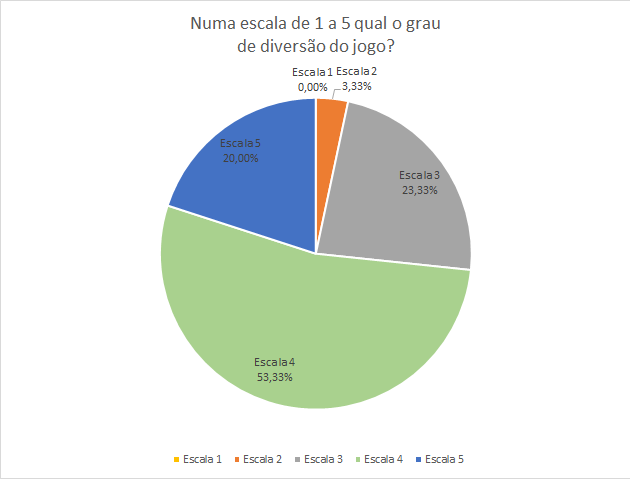
\includegraphics[scale=0.7]{./img/chart_1-.png}
     \caption{Resultado da Pergunta 1}
     \label{fig:question1}
\end{figure}


\begin{figure}[!htb]
     \centering
     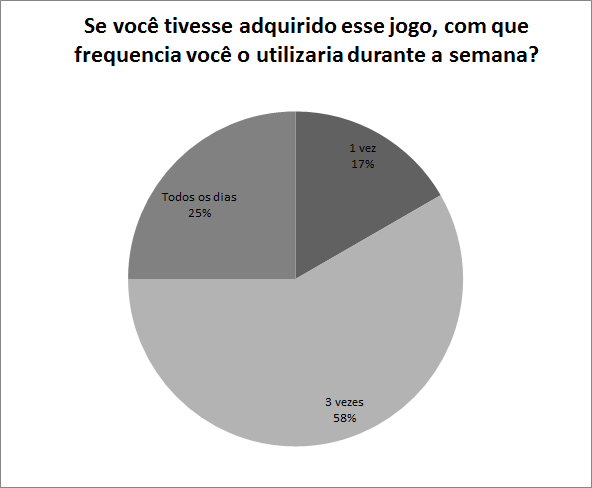
\includegraphics[scale=0.7]{./img/chart_3-.png}
     \caption{Resultado da Pergunta 3}
     \label{fig:question3}
\end{figure}
cathocatho

\begin{figure}[!htb]
     \centering
     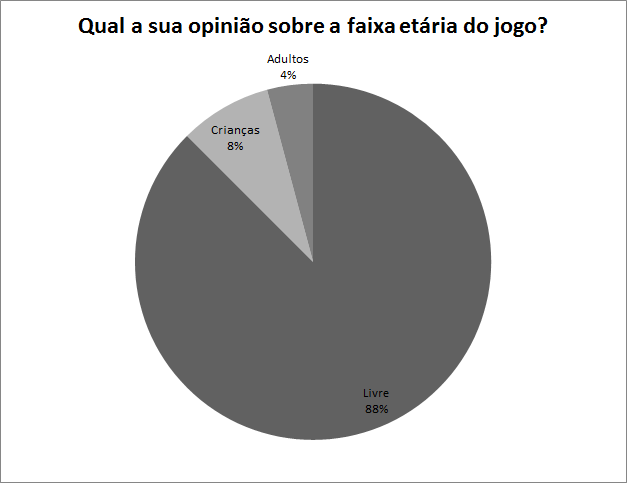
\includegraphics[scale=0.7]{./img/chart_10-.png}
     \caption{Resultado da Pergunta 10}
     \label{fig:question10}
\end{figure}
\FloatBarrier

De acordo com o resultado da avaliação dos usuários usando~\ac{gqm}, identificamos que a abordagem de um~\ac{sms} dos sinais motores usando jogos, como interface de entrada de dados, conseguiu motivar o usuário  a fornecer sinais motores e permite o acompanhar o tratamento a partir dos dados biomecânicos adquiridos. Logo, conseguimos atingir o principal objetivo da tese, ao demonstrar o monitoramento dos pacientes com~\ac{dp} de uma maneira não invasiva e no conforto de seus lares.

%\subsection{Conclusão} 
%Nessa etapa, buscou-se demonstrar que podemos desenvolver um jogo com mecanismos de captura de dados motores embutidos e que permita monitorar e quantificar sinais do Parkinson de uma maneira não-invasiva. 





\chapter{Conclusões e Trabalhos Futuros}\label{chapter:conclusoes_futuros}
Neste capítulo são apresentadas as conclusões sobre o trabalho apresentado e propostos trabalhos.  

%Já na Seção~\ref{sec:trab_futuros} são propostos possíveis trabalhos futuros. Por fim, no final do capítulo apresentamos as considerações finais na Seção~\ref{sec:cons_finais}.

Nos experimentos realizados, conseguimos demonstrar junto à comunidade de saúde (Seção~\ref{sec:entrevista_semi_estruturada}), a importância do acompanhamento dos sinais motores integrados à rotina diária do paciente. Identificou-se também, a importância de acompanhar a amplitude do movimento e a sua respectiva velocidade angular para acompanhamento da saúde motora.

Os estudos de aprendizagem de máquina com os dados motores adquiridos por meio de sensores de movimento usados em jogos eletrônicos, identificou a viabilidade do desenvolvimento de jogos para o monitoramento, pois, obtivemos uma taxa de acurácia de 86,67\% e falsos positivos de 6,67\% . A~\ac{svm} foi a técnica estatística de aprendizagem utilizada para distinguir os movimentos executados por indivíduos diagnosticados com~\ac{dp} ante os indivíduos de grupo controle. Esse estudo não teve a pretensão de estabelecer um diagnóstico da \ac{dp}, ou até mesmo provar que os movimentos utilizados pelos participantes da pesquisa servem para um diagnóstico. Contudo, este trabalho demonstrou que as diferenças nos movimentos, entre essas duas classes, permitem a identificação do sinal da bradicinesia, e que essas diferenças podem ser adquiridas por um sensor de movimento usado em jogos eletrônicos. A presente abordagem pode ser aplicada a outras doenças motoras; no entanto, testamos somente com indivíduos com~\ac{dp} e grupo controle.

Para identificar a possibilidade de integrar o monitoramento da saúde do jogador através de jogos eletrônicos à sua rotina diária, foi utilizada a análise \textit{Goal, Question, Metric} (GQM)~\cite{basili94} para avaliar a possibilidade de monitorar dados motores de forma não invasiva e integrada a rotina diária das pessoas. As métricas da análise quantificaram que um percentual de 90\% de usuários integrariam em sua rotina a solução de monitoramento proposta. Deve-se levar em consideração, também, que as métricas obtidas nessa pesquisa foram extraídas de um protótipo de jogo, e, caso este fosse aperfeiçoado é possível que a aceitabilidade da abordagem seja ainda maior. Desta maneira, conseguimos atingir o principal objetivo deste trabalho, ao permitir que indivíduos com comprometimento motor pudessem ser monitorados de maneira não-invasiva e no conforto de seus lares.




\subsubsection{Publicações}
Foram publicados três artigos, em conferências internacionais, relacionados à tese: 
  \begin{itemize}
   \item \textit{Abstract}: \textit{Monitoring Parkinson related Gait Disorders with Eigengaits}, no, \textit{XX World Congress on Parkinson's Disease and Related Disorders} (2013)~\cite{lmmeigengaits2013};
   \item \textit{Full Paper}: \textit{A Game-Based Approach to Monitor Parkinson’s Disease: The bradykinesia symptom classification}, no, \textit{International Symposium on Computer-Based Medical Systems} (CBMS 2016)~\cite{lmmcbmsgame2016};
   \item \textit{Full Paper}: \textit{A Gait Analysis Approach to Track Parkinson’s Disease Evolution Using Principal Component Analysis}, no, \textit{International Symposium on Computer-Based Medical Systems} (CBMS 2016)~\cite{lmmcbmsgait2016}.
  \end{itemize}

A partir dos resultados apresentados nesta tese e extensão da mesma, alguns trabalhos futuros são propostos para contribuição científica.

Como foi explanado na Seção~\ref{section:escalas_avaliacao}, a abordagem permite monitorar a progressão da doença e a eficácia do tratamento medicamentoso~\cite{updrs87,goul05}. Desta forma, é importante coletar uma amostra maior de pacientes com~\ac{dp}, agrupá-los de acordo com o estágio da doença~\cite{goul05}, e aplicar técnicas de multi-classificação de dados~\cite{multisvm2011} para identificar o progresso do~\ac{dp} de acordo com as escalas de avaliação. Em decorrência das ``Flutuações Motoras''~\footnote{Referente a respostas motoras flutuantes ao tratamento medicamentoso, com encurtamento da duração de seu efeito (fenômeno do \textit{wearing off}) e interrupção súbita de sua ação.}~\cite{protpar010},  é necessário comparar o sinal da bradicinesia em diferentes momentos do dia, para verificar a eficácia do tratamento medicamentoso~\cite{protpar010}.

Nos estudos realizados com os sinais adquiridos pelo MS-Kinnect, foi possível identificar a amplitude como apresentamos no estudo do movimento de abdução e adução do braço (Seção~\ref{sec:resultado_obtido_svm}). Todavia, a captura de um movimento mais sutil como um tremor é um desafio. Por esse motivo, foi desenvolvido e testado um jogo para celular que pudesse adquirir o sinal de tremor (Seção~\ref{sec:tremor}). Contudo, como o tremor do~\ac{dp} é de repouso~\cite{protpar010}, não foi possível quantificar o sinal. No entanto, ao analisarmos os vídeos dos pacientes com~\ac{dp}, identificamos, que ao levantar um dos membros, alguns indivíduos iniciavam o sinal de tremor no membro parado. Desta maneira, pode ser possível quantificar o sinal de tremor na análise do membro em repouso. No entanto, devido ao ruído existente na aquisição do sinal pelo MS-Kinnect~\cite{kinnect2013} pode-se inviabilizar a quantificação deste sinal. Como trabalhos futuros, uma investigação aprofundada destas questões podem gerar maiores contribuições para a área.













%%%%%%%%%%%%%%%%%%%%%%%%%%%%%%%%%%%%%%%%%%%%%%%%%%%%%%%%%%%%%%%%%%%%%%%%%%%%%%%%
%% Bibliografia
%% Coloque suas referencias no arquivo ref.bib e descomente as proximas duas linhas
%\bibliographystyle{plain}
%\bibliographystyle{unsrt}
\bibliographystyle{babplain}


%\bibliographystyle{plain}
\bibliography{biblmmcor}

%%%%%%%%%%%%%%%%%%%%%%%%%%%%%%%%%%%%%%%%%%%%%%%%%%%%%%%%%%%%%%%%%%%%%%%%%%%%%%%%
%% Apendice
% Caso seja necessario algum apendice, descomente a proxima linha.
\appendix

\chapter{Projeto do Comitê de Ética} \label{sec:comite}
\section{Resumo}
Com os recentes avanços na tecnologia de sensores sem fio, é possível incorporá-los na roupa ou no corpo (\textit{wearable}) do usuário e isso proporciona uma monitorização contínua dos sinais vitais. Contudo a concepção de um sistema de monitoramento \textit{wearable} que não seja invasivo ainda é um grande desafio. Por outro lado, a necessidade de integrar diferentes sensores em uma única solução dificulta essa atividade, pois os dispositivos são considerados pesados, visíveis e estereotipados pelos próprios usuários ~\cite{aarhus_negotiating_2010}, por esse motivo esses dispositivos são refutados, inviabilizando o monitoramento contínuo da saúde nesses casos. Contudo, desde 2005 os jogos eletrônicos fazem uso de dispositivos como acelerômetros, giroscópio, dispositivos de captura de movimento possibilitando ao usuário estivesse uma maior imersão no universo do jogo através da análise de seus movimentos. Esses sensores usados em jogos eletrônicos permitem capturar sinais  de tremores ~\cite{synnott_wiipd_
2012,lemoyne2010} 
e posturais que são sintomas presentes no \ac{dp}. Como o uso desses dispositivos já está embutido no contexto do jogo, possivelmente o usuário não iria sentir desconforto caso fossem usados para monitorar os sintomas do \ac{dp} enquanto estivesse num momento de descontração ao usar um jogo eletrônico. 

\section{Introdução}
A \ac{dp} é uma das doenças mais comum nos idosos. Apesar dos sintomas clássicos o diagnóstico clínico não é específico, não há exames laboratoriais, diagnósticos e existem outras doenças que se manifestam como o \ac{dp} ~\cite{vedolin2003,tolosa06}. O \ac{dp} é uma afecção do sistema nervoso central, a qual é expressa de forma crônica e progressiva. Ela é causada pela degeneração dos neurônios produtores de dopamina presente na substância negra e caracterizada pelos sintomas parkinsonianos: tremor em repouso (que diminui durante movimentos voluntários); bradicinesia ou hipocinesia (lentidão e escassez de movimentos, além de dificuldade na marcha), rigidez muscular (aumento da resistência ao movimento passivo dos membros), perda de reflexos posturais que leva a alteração da marcha e aumenta a ocorrência de queda ~\cite{tolosa06,rodrigues2006}. 

Parkinsonismo é um termo genérico que designa uma série de doenças com causas diferentes e que têm em comum a presença de sintomas frequentemente encontrados no~\ac{dp}. Esta doença é uma das muitas formas de parkinsonismo, correspondendo a cerca de 75$\%$ dos casos. A evolução da doença a gravidade e a progressão dos sintomas variam de um paciente para outro. No momento não existe teste diagnóstico para a doença e estudos comprovam dificuldade na diferenciação clínica entre \ac{dp} e outras formas de parkinsonismo. A maioria dos neurologistas concorda que o diagnóstico do \ac{dp} requer a identificação de alguma combinação de sinais motores cardinais (tremor de repouso, bradicinesia, rigidez tipo roda denteada, alterações posturais), porém uma classificação clínica padrão ainda não foi obtida ~\cite{protpar010}. Além do mais, um diagnóstico auxiliar importante é a resposta dos pacientes aos medicamentos antiparkinsonianos tal como a levodopa ~\cite{protpar010}. Os pacientes com~\ac{dp} quase 
sempre apresentam uma resposta satisfatória a esse medicamento, e no caso de não responder satisfatoriamente à levodopa, é provável que o diagnóstico seja de outra forma de parkinsonismo. Porém, na literatura ~\cite{rowlandtratado} uma resposta à levodopa não confirma o diagnóstico do \ac{dp} porque existem muitos casos de parkinsonismo sintomático e muitas formas de síndrome de Parkinson em seus estágios iniciais que também respondem à levodopa. 

O \ac{dp} é uma doença mais comum em idosos, porém existem casos precoces de início da doença em indivíduos antes dos 40 anos ou até mesmo abaixo dos 21 ~\cite{menezes2003}. A incidência da doença é estimada de 100 a 200 casos por 100.000 habitantes, com o avanço da idade a probabilidade do desenvolvimento da doença tende a aumentar. Por se tratar de uma doença progressiva, sua evolução acarreta em incapacidade grave após 10 a 15 anos, ocasionando em impacto social e financeiro, principalmente na população mais idosa. Estima-se que o custo anual mundial com medicamentos antiparkinsonianos esteja em torno de 11 bilhões de dólares, sendo o tratamento cerca de 3 a 4 vezes mais caro para pacientes na fase avançada da doença ~\cite{protpar010}.

Com o surgimento do tratamento para o \ac{dp} torna possível manter uma boa mobilidade funcional durante anos e aumenta a expectativa de vida dos pacientes tratados ~\cite{rodrigues2006}. Os fármacos do grupo dos antiparkinsonianos como a levodopa permitiram restaurar a atividade dopaminérgica que pode se encontrar reduzida, desta forma as drogas utilizadas são bem sucedidas no alívio de sintomas característicos da doença. Entretanto, devido aos efeitos colaterais frequentes induzidos pelos fármacos, é preciso iniciar o tratamento com esses medicamentos somente quando os sintomas estiverem prejudicando o desempenho profissional ou das atividades diárias do paciente ~\cite{rodrigues2006}.

A natureza progressiva do \ac{dp} e suas manifestações clínicas (motoras e não motoras),  associadas a efeitos colaterais precoces e tardios da intervenção terapêutica, tornam o tratamento da doença bastante complexo ~\cite{protpar010} e estima-se que a taxa de morte dos neurônios dopaminérgicos da substância negra situa-se  ao redor de 10$\%$ ao ano~\cite{national2006parkinson}. Consequentemente, com o passar do tempo a sintomatologia parkinsoniana piora necessitando aumentar as doses da medicação, logo com a progressão da doença, a eficácia do tratamento diminui e os pacientes passam a não responder ao tratamento medicamentoso ~\cite{protpar010}. 

Alternar entre os estados \textit{on} (``normal'') e \textit{off} (``com os sintomas parkisonianos''). As mudanças dos estados \textit{on} para \textit{off} dependerá do horário da ingestão do medicamento que tornará previsível a mudança para o estado \textit{on}. Contudo, alguns pacientes podem ter mudanças abruptas para o estado \textit{off}, sem qualquer correlação com o tempo em que a medicação foi ingerida. Essa irregularidade de não conseguir determinar o momento em que o paciente entrará no estado \textit{on} ou \textit{off} impacta diretamente nas avaliações objetivas do profissional que irá avaliar a evolução da doença ~\cite{kostek12,patel_monitoring_2009}. 

Outro efeito colateral no uso do medicamento bastante conhecido é o surgimento da discinesia (movimentos involuntários de contorção) em 80$\%$ dos pacientes que recebem a levodopa como tratamento prolongado. Esse sintoma pode ser aliviado com a diminuição da dose, por outro lado, os sintomas da doença tendem a retornar. Com o surgimento de discinesia intensa é necessário otimizar o gerenciamento do tratamento medicamentoso, levando a adicionar novos medicamentos para reduzir os sintomas incapacitantes a longo prazo ~\cite{rodrigues2006}. 

A partir dos tratamentos para o \ac{dp}, foram criadas escalas de avaliação do progresso da doença ~\cite{updrs87,Hoehn_Yahr_2001}. Essas escalas permitem avaliar: a condição clínica geral, incapacidades, funções motoras e mentais e até mesmo a qualidade de vida dos pacientes. Esses instrumentos são importantes tanto no nível clínico quanto no científico, pois permitem monitorar a progressão da doença e a eficácia do tratamento medicamentoso ~\cite{updrs87,goul05}.  Sendo assim, foi criada em 1987 a Escala Unificada de Avaliação da  Doença de Parkinson (Unified Parkinson’s Disease Rating Scale – UPDRS) ~\cite{updrs87} que é amplamente utilizada para monitorar a progressão da doença e a eficácia do tratamento, sendo considerada confiável, válida e qualificada como um método adequado para a avaliação do~\ac{dp} ~\cite{goul05}. 

% 
% Atualmente a evolução da \ac{dp} é avaliada através de escalas, que permitem avaliar a eficácia do tratamentos e sua aplicabilidade nas práticas fisioterápicas. Segundo um trabalho de Goulart ~\cite{goul05} as escalas de estágios de incapacidade representadas por Hoehn/Yahr ~\cite{Hoehn_Yahr_2001} e a UPDRS ~\cite{updrs87} são consideradas as de maior confiabilidade, podendo ser usadas por fisioterapeutas para melhor avaliação do estado clínico-funcional do  paciente.

Na UPDRS a evolução do~\ac{dp} é classificada nas seguintes fases ~\cite{updrs87}:
  \begin{itemize}
    \item \textbf{ESTÁGIO 0:} Nenhum sinal da doença;
    \item \textbf{ESTÁGIO 1:} Doença unilateral;
    \item \textbf{ESTÁGIO 1,5:} Envolvimento unilateral e axial;
    \item \textbf{ESTÁGIO 2:} Doença bilateral sem déficit de equilíbrio;
    \item \textbf{ESTÁGIO 2,5:} Doença bilateral leve, com recuperação no “teste do empurrão”;
    \item \textbf{ESTÁGIO 3:} Doença bilateral leve a moderada; alguma instabilidade postural; capacidade para viver independente;
    \item \textbf{ESTÁGIO 4:} Incapacidade grave, ainda capaz de caminhar ou permanecer de pé sem ajuda;
    \item \textbf{ESTÁGIO 5:} Confinado à cama ou cadeira de rodas a não ser que receba ajuda.
  \end{itemize}

A UPDRS é composta por 42 itens, divididos em quatro partes (atividade mental, comportamento e humor, atividades de vida diária e exploração motora e complicações da terapia medicamentosa) e através da avaliação desses sintomas, por intermédio do auto-relato e da observação clínica, é possível classificar em que estágio da doença o paciente se encontra. Contudo, justamente por ser baseada em auto-relato e observação clínica a qual é realizada eventualmente com a presença de um profissional, pesquisadores questionam a efetividade da avaliação do estágio da doença e propõem alternativas para avaliação dos itens motores de forma quantitativa através de sensores, os quais permitem monitorar o estágio do paciente ~\cite{kostek12,synnott_wiipd_2012,patel_monitoring_2009}.


A identificação dos sintomas do \ac{dp} durante a rotina diária permite um diagnóstico mais precoce da doença e consequentemente obter seus benefícios de um tratamento mais duradouro. Além disso, o monitoramento dos efeitos da medicação usada pelo paciente permite um gerenciamento da medicação e consequentemente reduz os sintomas indesejáveis da doença e prolongando a qualidade de vida do paciente.

Com os recentes avanços na tecnologia de sensores sem fio, é possível incorporá-los na roupa ou no corpo (\textit{wearable}) do usuário e isso proporciona uma monitorização contínua dos sinais vitais. Contudo a concepção de um sistema de monitoramento \textit{wearable} que não seja invasivo ainda é um grande desafio ~\cite{alemdar}. Por outro lado, a necessidade de integrar diferentes sensores em uma única solução dificulta essa atividade, pois os dispositivos são considerados pesados, visíveis e estereotipados pelos próprios usuários ~\cite{aarhus_negotiating_2010}, por esse motivo esses dispositivos são refutados, inviabilizando o monitoramento contínuo da saúde nesses casos. Contudo, desde 2005 os jogos eletrônicos fazem uso de dispositivos como acelerômetros, giroscópio, dispositivos de captura de movimento possibilitando ao usuário estivesse uma maior imersão no universo do jogo através da análise de seus movimentos. Como visto na literatura científica, esse sensores usados em jogos eletrônicos permitem 
capturar sinais de tremores~\cite{synnott_wiipd_2012,lemoyne2010} e posturais que são sintomas presentes no \ac{dp}. Como o uso desses dispositivos já está embutido no contexto do jogo, possivelmente o usuário não iria sentir desconforto caso fossem usados para monitorar os sintomas do \ac{dp} enquanto estivesse num momento de descontração ao usar um jogo eletrônico. 

Os jogos eletrônicos não são usados somente por crianças e adolescente, em uma pesquisa da Entertainment Software Association, associação formada pelas principais fabricantes americanas de jogos eletrônicos \textit{``Essential Facts About the Computer and Video Game Industry"}~\cite{esa2011} demonstra que em 2011 os jogadores de videogame dos Estados Unidos possuem, em média, 37 anos e 29$\%$ dos jogadores de videogame possuem mais de 50 anos. Logo, temos uma parcela bastante significativa de usuários que podem ser beneficiados com o monitoramento de dados de saúde por intermédio dos jogos eletrônicos.

%fazer a figura
Como visto, o objetivo principal deste trabalho é possibilitar meios de monitorar o usuário e tentar identificar sintomas do \ac{dp} em diferentes momentos do dia com o propósito de possibilitar um diagnóstico precoce e melhorar no gerenciamento da dosagem medicamentosa contribuindo para um prolongamento da qualidade de vida dos pacientes com \ac{dp}.

% 
\section{Problemática}
Alinhar a jogabilidade e a possibilidade de monitoramento dos dados de saúde não é uma tarefa trivial. Pois deve ser levado em consideração o uso dos dispositivos e pensar na execução de movimentos ou ações que permitam esse monitoramento. Os movimentos não podem ser repetitivos pois, levaria o usuário jogar por um curto período e como consequência abandonaria o monitoramento ~\cite{Suhonen:2008:SFE:1457199.1457204}. Para propor um jogo que consiga obter um monitoramento dos dados de saúde, deve ser realizado um estudo sobre quais os movimentos e ações que o usuário deve executar. Posteriormente, na posse dessas ações, deverá ser testada a execução dessas atividades e sua captura e possível classificação conforme os trabalhos já existentes que realizam essas atividades~\cite{Ballegaard:2008:HEL:1357054.1357336,albanese2012,bachlin_parkinsons_2009,visionbased2009,patel_monitoring_2009}. De posse dos movimentos e da captura dos dados será feito um levantamento de um \textit{game design} que permita executar os 
movimentos em  um ambiente lúdico e divertido como um jogo para entretenimento ~\cite{sweetser2005-gameflow}.


\section{Objetivo}
Essa pesquisa tem como objetivo identificar sintomas motores da doença de parkinson (tremores, bradicinesia e discinesia) através de um jogo eletrônico, dentro de um grupo de casos com doença de parkinson em diferentes estágios da doença segundo a UPDRS ~\cite{updrs87}.


\subsection{Específicos}
\begin{itemize}
 \item Capturar a  manifestação clínica de bradicinesia em casos de parkinson ao mover-se de um lado para o outro, levantar o braço e a perna através do uso de um dispositivo de captura de vídeo e reconhecimento de movimentos;
 \item Capturar os movimentos do grupo controle ao mover-se de um lado para o outro, levantar o braço e a perna através do uso de um dispositivo de captura de vídeo e reconhecimento de movimentos;
 \item Verificar a relação entre a manifestação do sintoma de bradicinesia em efeito com o medicamento antiparkinsoniano através do uso de um dispositivo de captura de vídeo e reconhecimento de movimentos;
\end{itemize}

\section{Material E Métodoo}

\subsection{Tipo de Estudo}
Estudo analítico de caso-controle.


\subsection{Local}
Grupo de pacientes da Clínica de Fisioterapia Dr. Rodrigo Ramalho pertencente ao Centro Universitário Cesmac.


\subsection{Amostra}
A técnica de amostragem utilizada para seleção, será por conveniência onde será composta por todos indivíduos que estejam diagnosticado com \ac{dp} e indivíduos da mesma faixa etária como grupo de controle.

\subsection{Formas de Recrutamento}
A forma de recrutamento deste protocolo será Circunscrita por intermédio de um profissional de saúde da própria Clínica de Fisioterapia. O profissional deverá conhecer a história clínica do paciente e obterá a permissão do mesmo para que a equipe de pesquisa possa entrar em contato.
A equipe de pesquisa deverá explicitar os riscos e benefícios da participação da pesquisa buscando a espontaneidade da decisão e depois fornecer o Termo De Consentimento Livre E Esclarecido.


\subsubsection{Critério de inclusão}
Casos com a \ac{dp} diagnosticada até o estágio 3 segundo a UPDRS ~\cite{updrs87}, sem distinção de sexo ou raça, que esteja com participação ativa na Clínica de Fisioterapia Dr. Rodrigo Ramalho e que aceitem participar do estudo.

\subsubsection{Critério de exclusão}
Pessoas com sintomas motores que não sejam do \ac{dp} e que tenham problemas em equilíbrio além daqueles que se neguem a participarem do estudo.

\subsection{Material}
Para a presente pesquisa serão testados dois jogos desenvolvidos por alunos do Instituto Federal de Alagoas (IFAL) e da Universidade Federal de Campina Grande (UFCG).

%\subsubsection{Jogo: Pinball World}
%O \textit{Pinball World}, é um jogo voltado para o entretenimento e pode ser usado por seus usuários em diferentes momentos do dia. O principal propósito do jogo é monitorar os sintomas de tremor das mãos do usuário por intermédio do acelerômetro usado como instrumento de controle. O usupário deverá movimentar o dispositivo para esquerda, direita e isso controlará a bola de \textit{pinball}, personagem principal do jogo. Durante o jogo o nível de tremor em movimento do usuário capturado e em outro momento em que o usuário precisa apenas visualizar o trajeto da bola, o jogador permanecerá parado e nesse momento será possível capturar o tremor de repouso. O jogo é composto por uma floresta e com  uma cachoeira e sua respectiva queda d'agua trazendo paz e tranquilidade ao jogador.
%
%O tremor de movimento é capturado durante os momentos em que o jogador precisa movimentar o dispositivo para controlar a bola e desviar de obstáculos. Em outro momento, quando o jogador mantém o dispositivo parado e precisa apenas visualizar o trajeto da bola, é possível capturar o tremor de repouso. As coordenadas do acelerômetro são capturadas a uma taxa de amostragem de 16Hz durante o curso do jogo. De acordo com a Tabela~\ref{tab:tremors}~\cite{albanese2012}, uma taxa de amostragem de 16Hz é suficiente para capturar os tipos de tremores que ocorrem nas mãos e membros. 
%
%
%\begin{figure}[!htb]
     %\centering
     %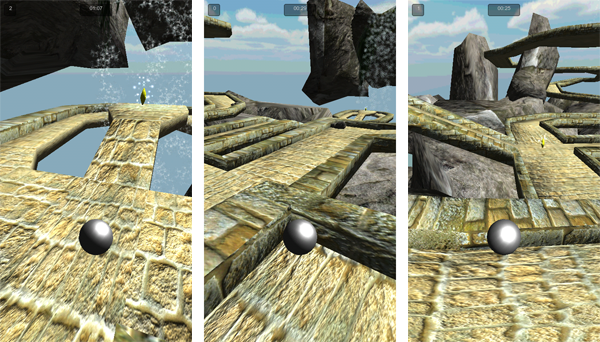
\includegraphics[scale=.6]{pinball_world.png}
     %\caption{O Jogo \emph{Pinball World}}
     %\label{img:pw1}
%\end{figure}
%
%\begin{table} 
%\centering 
%\caption{Tipos de tremor, diferenciados pela frequência, amplitude e início em relação a movimentos voluntários}
%\begin{center}
    %\begin{tabular}{ | l | p{2.5cm} | p{2.5cm} | p{2.5cm} | p{3.5cm} | }
        %\hline
        %Frequência & Tipo de tremor & Amplitude & Lado predominante & Relação com movimento voluntário \\ \hline
        %1-4 Hz & Cerebelar & Média-Alta & Membros & Postural, ação \\ \hline
        %3-5 Hz & Específico de tarefa & Baixa-Média & Mão & Escrita, segurar talheres, tocar instrumentos \\ \hline
        %4-5 Hz & Parkinsoniano & Média-Alta & Membros, mandíbula & Repouso \\ \hline
        %5-8 Hz & Essencial & Média-Alta & Membros, cabeça, voz & Postural \\ \hline
        %8-12 Hz & Fisiológico & Média & Membros & Postural \\ \hline
        %14-16 Hz & Ortostático & Baixa-Média & Pernas, tronco & Ficar de pé \\ \hline
    %\end{tabular}
%\end{center}
%\label{tab:tremors}
%\end{table}

\subsubsection{Jogo: \textit{Catch the Spheres}}
O jogo \textit{Catch the Spheres} é em terceira pessoa no qual o jogador, por meio de seu personagem, deverá capturar ou desviar de bolas que vêm em sua direção. Existem dois tipos de bolas: azuis e vermelhas. Inicialmente, todas as bolas são vermelhas e algumas destas mudam para a cor azul ao se aproximarem do jogador. O tempo para a bola mudar de cor pode ser menor ou maior, a depender do nível de dificuldade selecionado. Um personagem no centro do cenário replica todos os movimentos executados pelo jogador e capturado através do dispositivo de captura de vídeo. Deve-se tocar as bolas azuis com os pés ou as mãos e desviar das bolas vermelhas.

%\begin{figure}[!htb]
     %\centering
     %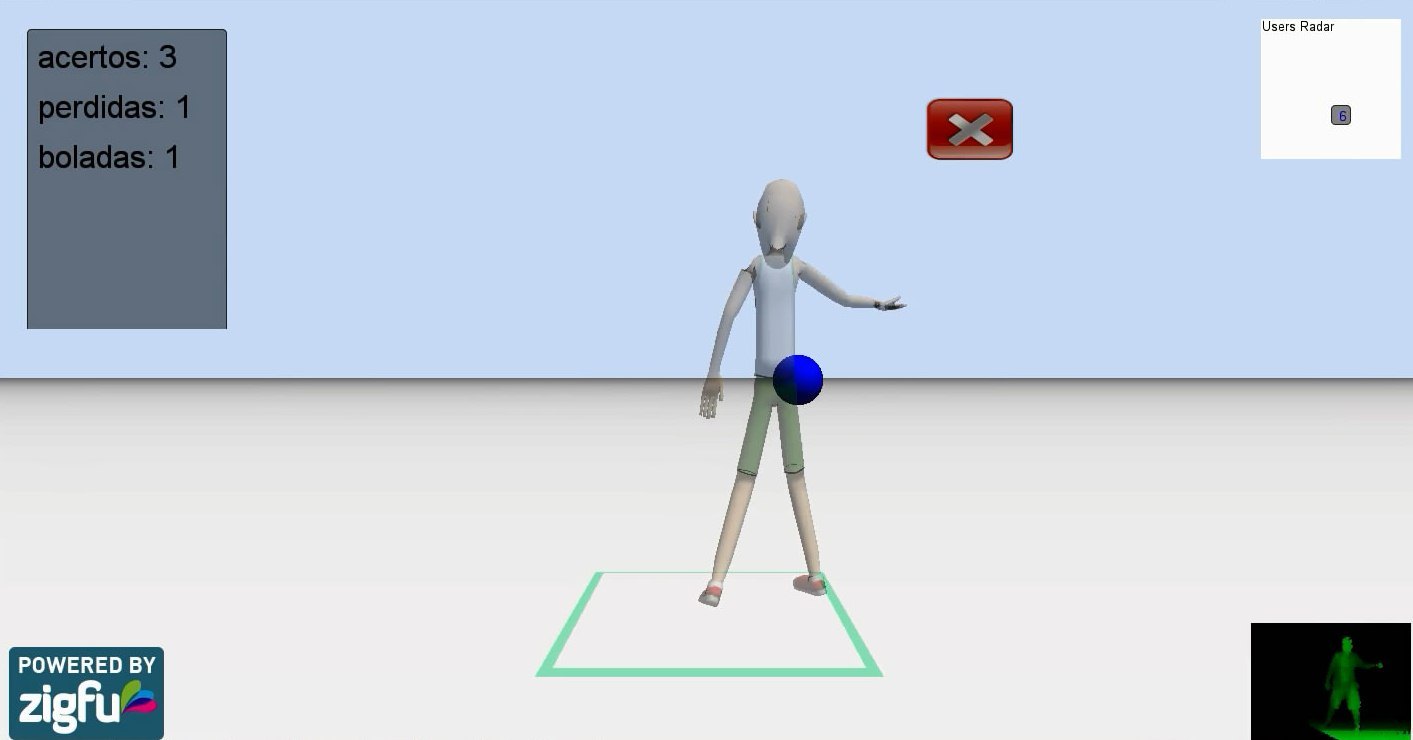
\includegraphics[width=.8\textwidth]{catch-the-spheres.jpg}
     %\caption{O jogo \emph{Catch the Spheres}}
     %\label{img:catch}
%\end{figure}

\begin{figure}[!htb]
     \centering
     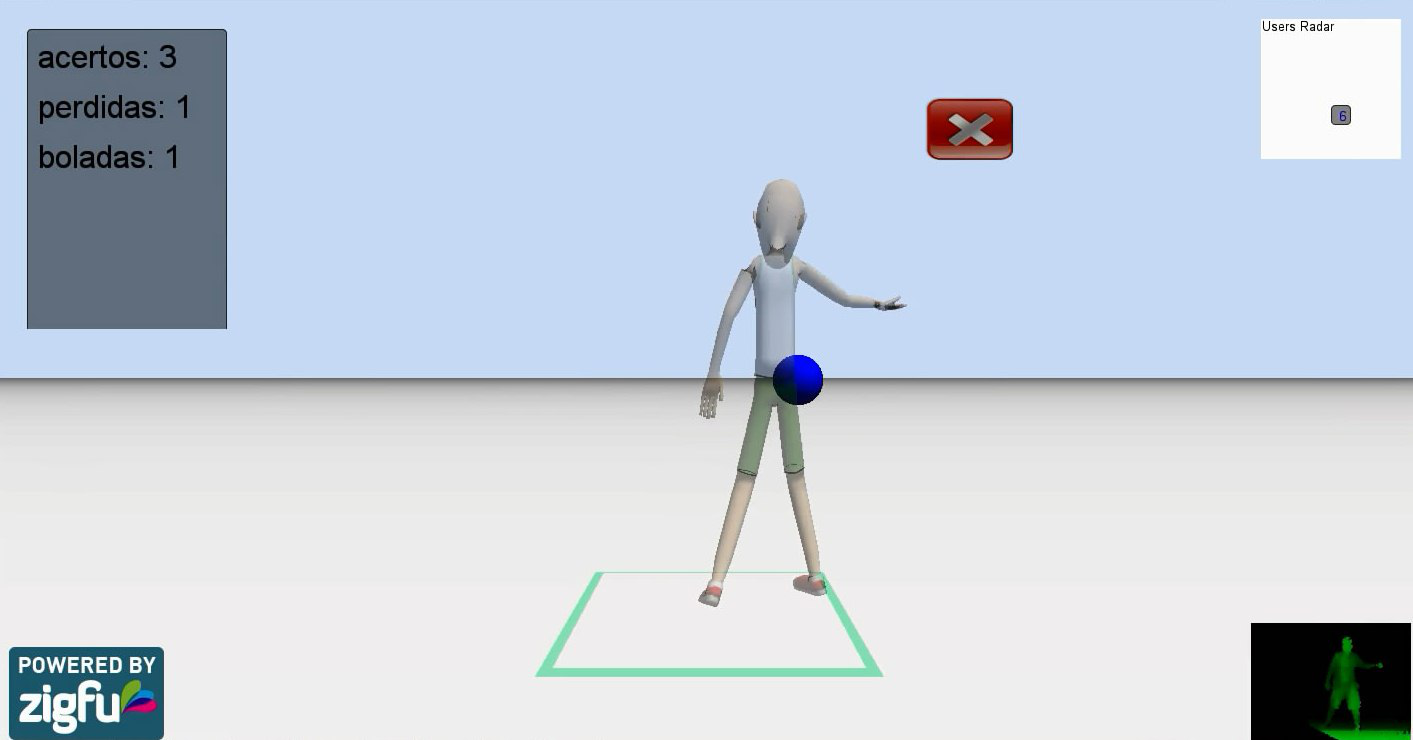
\includegraphics[width=.8\textwidth]{./img/catch-the-spheres.png}
     \caption{O jogo \emph{Catch the Spheres}}
     \label{img:catch}
\end{figure}

A finalidade do jogo é capturar dados do movimento do jogador enquanto ele executa as ações específicas do jogo. O intervalo de tempo entre o momento em que a bola muda de cor e o momento em que a bola é capturada pelo jogador mede o reflexo do jogador, enquanto que a velocidade dos seus membros é calculada através da distância percorrida pelas mãos ou pés para capturar as bolas.
Com a execução desse jogo, pretende-se colher dados para conseguir identificar os sintomas do \ac{dp} como bradicinesia.



\subsection{Procedimentos}

Este protocolo de pesquisa será submetido à avaliação do Comitê de Ética em Pesquisa do Centro Universitário Cesmac, somente depois da aprovação deste é que os dados serão coletados.

Para identificar a possibilidade de integrar o monitoramento da saúde do jogador por intermédio de jogos eletrônicos à sua rotina diária, será utilizada a abordagem \textit{Goal, Question, Metric} (GQM). GQM é uma abordagem hierárquica que inicia com objetivo principal e o divide em atividades que podem ser mensuradas durante a execução do projeto. É uma abordagem para integrar objetivos a modelos de processos de software, produtos e perspectivas de qualidade de interesse, baseado nas necessidades do projeto e da organização~\cite{van1999goal}. Os participantes da pesquisa serão convidados a responder o questionário GQM para avaliar se o jogo permite monitorar dados motores de forma não invasiva podendo estar integrado a rotina diária das pessoas.

%Os resultados que se desejam alcançar será o descobrimento de mecanismos para a identificação e classificação dos sintomas de tremores. O tremor é o principal sintoma parkinsoniano e a diferença dos ciclos pode auxiliar no diagnóstico da doença; sua maior frequência é quando o membro está em repouso sendo chamado de tremor de repouso.
Essa pesquisa também fará uma análise de jogos que fazem uso de sensores de movimento e avaliará as possibilidades de aquisição de dados de saúde baseada na Cinemática Angular do Movimento Humano. Através dos resultados obtidos pretendemos avaliar e classificar a normalidade e dificuldade na %execução de movimentos como levantar um braço, esticar uma perna ou balançar o corpo.
execução de movimentos como levantar um braço.

A coleta de dados será feita no próprio espaço sendo realizada em local reservado e de forma individual e permitindo sua participação por meio do Termo de Consentimento.

Os voluntários da pesquisa deverão executar os seguintes procedimentos:
\begin{enumerate}
	\item O voluntário irá jogar o jogo \emph{Catch the Spheres} por aproximadamente 1 minuto e 30 segundos;
	%\item O voluntário irá jogar o jogo \emph{Pinball World} com apenas uma das mãos por aproximadamente 1 minuto e 30 segundos; 
	\item Responder o questionário GQM.
\end{enumerate}

\subsubsection{ANÁLISE DE DADOS}


\subsection{Base de Dados}
Todos os dados coletados através do acelerômetro e dispositivos de vídeo serão disponibilizados para pesquisa futura, permitindo o uso para pesquisa a todas Instituições envolvidas (CESMAC, UFCG, UFAL e IFAL). Contudo, conforme informado no Termo de Consentimento Livre e Esclarecido, será preservada a identidade do participante na pesquisa e todos os dados que possibilitem sua identificação serão omitidos.


\subsection{Termo de Consentimento Livre e Esclarecido (TCLE)}
O participante consentirá com sua participação através da assinatura do Termo de Consentimento Livre e Esclarecido. O mesmo receberá todas as informações necessárias quanto à realização do estudo em todas as suas etapas. Estará cientificado de que sua participação será de acordo com sua vontade, podendo desistir quando lhe aprouver. O termo de consentimento livre e esclarecido se baseia na Resolução Nº 196/96, do Conselho Nacional de Saúde, do Ministério da Saúde (CNS/MS), devendo ser assinado pelo mesmo antes de ser inserido no estudo, procedimento este realizado pelo pesquisador responsável.

\subsection{Confidencialidade}
Os dados do estudo em questão serão considerados propriedade conjunta das partes envolvidas, não devendo ser comunicados a terceiros por uma das partes sem prévia autorização da outra parte interessada. No entanto, torna-se expresso, o comprometimento em tornar público os resultados da pesquisa, sejam eles favoráveis ou não.

\subsection{Critérios Para Interromper a Pesquisa}
Os critérios específicos de interrupção ocorrerão de forma individual para cada sujeito. A pesquisa será interrompida caso os participantes desistam de fazerem parte do estudo, ou caso seja desrespeitado algum preceito ético.

\subsection{Relação Risco Benefício da Pesquisa}
Os riscos inerentes podem decorrer da exposição de dados dos sujeitos da pesquisa, o que pode acarretar danos morais e/ou psicológicos. Assim, serão tomados todos os cuidados para que a identidade do sujeito da pesquisa não seja revelada, garantindo assim, privacidade e confidência das informações. Assim todos os dados do estudo serão manipulados apenas principais pesquisadores, todos os dados serão armazenados sob criptografia, mitigando a possibilidade de vazamento da informação.

Caso surja algum constrangimento por parte do sujeito da pesquisa, ao não conseguir realizar a pesquisa ou responder alguma pergunta devido ao comprometimento da doença. Os pesquisadores prestarão total assistência, orientando adequadamente os sujeito da pesquisa.

O risco se justifica pelos benefícios que a pesquisa poderá trazer com a possibilidade de monitoramento dos sintomas do \ac{dp}. A identificação dos sintomas motores e classificação desses dados através do computador permitirá avanços para um melhor acompanhamento da evolução da doença além de permitir que os pacientes possam ser monitorados de forma não invasiva através de um jogo eletrônico. Os pacientes deverão ter o seu estágio do \ac{dp} previamente diagnosticada por um médico para ser possível comparar os dados do monitoramento com o diagnóstico obtido.

\subsection{Infra-Estrutura}
A pesquisa será realizada na Clínica de Fisioterapia Dr. Rodrigo Ramalho, onde são realizados tratamentos fisioterápicos juntamente com estudantes do curso de fisioterapia do CESMAC. O espaço físico oferece condições favoráveis e adequadas para aplicação dos jogos e também resposta do questionário GQM propostos para este estudo. Para a realização da pesquisa serão utilizados:
\begin{itemize}
  %\item Jogo rodando em celular \textit{smartphone} com Sistema Operacional Android 4.0;
  \item Jogo rodando em notebook com Sistema Operacional Windows 7.0 e Unity 3d 3.0;
  \item Caneta esferográfica;
  \item Papel;
  \item Pranchetas;
  \item Pastas arquivadoras;
\end{itemize}


\section{Etapas da Pesquisa e Cronograma} 

\subsection{Etapa da Pesquisa}
\begin{table}
 \centering
	\begin{tabular}{|c|c|}
		\hline Etapa I & Elaboração Projeto \\ 
		\hline Etapa II & Entrega à Coordenação para análise do Comitê de Ética \\ 
		\hline Etapa III & Coleta dos dados* \\ 
		\hline Etapa IV & Apuração e análise dos dados* \\ 
		\hline Etapa V & Identificação e Classificação dos Sintomas* \\ 
		\hline Etapa VI & Disponibilização dos Resultados* \\ 
		\hline 
	\end{tabular} 
	\label{etapas}
	\caption{Etapas da Pesquisa}
\end{table}

$\*$As datas previstas neste cronograma estão sujeitas a modificação, a depender da aprovação do CEP, onde só após esta serão iniciadas.

\subsection{Cronograma}
\begin{table}
	\centering
	\begin{tabular}{|c|c|c|c|c|c|c|}
		\hline Abril & X &  &  &  &  &     \\ 
		\hline Maio &  & X &  &  & &      \\ 
		\hline Junho &  &  & 0 & 0 &  &     \\ 
		\hline Junho &  &  &  & 0 & 0 &     \\ 
		\hline Julho &  &  &  &  & 0 &     \\ 
		\hline Agosto &  &  &  &  & 0 &    \\ 
		\hline Setembro &  &  &  &  &  & 0 \\ 
		\hline 
	\end{tabular} 
	\label{crono}
	\caption{Cronograma}
\end{table}
\textbf{Legenda: [0] Planejado [X] Executado}

\section{Orçamento Estimado} 
Todo o material permanente que será utilizado nesta pesquisa já é de posse do pesquisador principal. O material de consumo será adquirido com recursos próprios dos pesquisadores, que não irão honorários específicos para esta pesquisa.

\begin{table}
	\centering
	\begin{tabular}{|c|c|c|}
		\hline \textbf{ITEM} & \textbf{VALOR UNITÁRIO(R$\$$)} & \textbf{VALOR TOTAL (R$\$$)}\\ 
		\hline 1 Smartphone Samsung Gallaxy S3 & 1200,00 & 1200,00 \\ 
		\hline 1 Notebook com Windows 7 & 2000,00 & 2000,00 \\ 
		\hline 
	\end{tabular} 
	\label{material_permanente}
	\caption{Material Permanente}
\end{table}


\begin{table}
	\centering
	\begin{tabular}{|c|c|c|}
		\hline \textbf{ITEM} & \textbf{VALOR UNITÁRIO(R$\$$)} & \textbf{VALOR TOTAL (R$\$$)}\\ 
		\hline 1 Resma de Papel & 17,00 & 17,00 \\ 
		\hline 1 Tonnner Impressora a Laser & 50,00 & 50,00 \\ 
		\hline 4 Canetas esferográficas & 2,00 & 8,00 \\
		\hline 2 Pranchetas & 10,00 & 20,00 \\
		\hline 1 Pasta Arquivadora & 3,00 & 3,00 \\
		\hline 
	\end{tabular} 
	\label{material_permanente}
	\caption{Material de Consumo}
\end{table}

\textbf{TOTAL R$\$$: 1.782,00} \\
Todos os gastos acima relacionados serão custeados pelos pesquisadores responsáveis pelo estudo.


\chapter{Questionário Entrevista Semiestruturada} \label{apendice:entrevista-semi-estruturada}
% Palavras-chave do resumo em Português
%\begin{keywords}
%projetos de pesquisa, processo de desenvolvimento, processo de
%requisitos.
%\end{keywords}

\section{Entrevista com Profissionais de Neurologia}

Esse documento contém um conjunto de perguntas a serem respondidas em entrevistas semi-estruturadas, a profissionais que trabalham diretamente com doenças neurológicas envolvidos no acompanhamento de pacientes com a doença de parkinson. A pretensão dessa pesquisa é a identificação de mecanismos que auxiliem no monitoramento dos sintomas da doença para auxiliar os neurologistas no gerenciamento da dosagem do medicamento antiparkinsoniano.

\subsection{Sintomas da Doença de Parkinson}
\begin{itemize}
    \item Como é realizado o diagnóstico da doença de parkinson ?
		\item Quais são os sintomas mais frequentes ?
		\item Quais sintomas são amenizados pela dosagem medicamentosa ?
\end{itemize}

\subsection{Monitoramento de dados Motores}
\begin{itemize}
    \item O movimento  de adução e abdução do braço, é um movimento relevante para a identificação da doença de parkinson.
		\item É importante que o profissional de saúde acompanhe a amplitude máxima desses movimentos?
		\item Quão importante é monitorar a velocidade angular do movimento de adução em º/s para a avaliação do sintoma de bradicinesia da doença de parkinson ? Esse sintoma pode ser avaliado em outras doenças ? Cite exemplos.
		\item A doença de parkinson apresenta assimetria do movimento como um dos seus sintomas. Ou seja um lado do braço tem uma amplitude maior do que o outro lado.
		\item Demonstrar a amplitude máxima do movimento de abdução poderia ser aplicado para outras doenças que impactam na mobilidade? Cite exemplos ?		
		\item Um mecanismo que pudesse monitorar os sintomas da doença de parkinson como: tremor, bradicinesia e discinesia. Poderia auxiliar na eficácia da medicação?
		\item Qual a relação do tremor com o uso dos medicamentos antiparkinsonianos ?
		\item A bradicinesia e discinesia são influenciadas pelos medicamentos antiparkinsonianos ?
		\item As diretrizes médicas citam tabelas de evolução da doença de Parkinson como a UPDRS, você as utiliza na sua prática clínica?		
\end{itemize}

\subsection{Benefícios}
\begin{itemize}
    \item A literatura informa que a doença de parkinson é progressiva e devido ao uso de medicamentação estas passam a não surtir efeito necessitando aumentar a dosagem medicamentosa além de efeitos colaterais incapacitantes causados pelo uso da medicação. Diante desses problemas como a dosagem medicamentosa é definida para o paciente ?
		\item Como profissional,seria importante acompanhar: amplitude do movimento, velocidade angular de abdução, velocidade angular de adução?
		\item Esses valores permitiriam visualizar a melhora ou o comprometimento do paciente?
		\item Você acha interessante ser auxiliado por uma máquina de aprendizagem que análise esses dados para facilitar o seu trabalho e melhorar na avaliação dos pacientes ?
		\item Sabendo que muitos indivíduos usam jogos eletrônicos em sua rotina, supondo que dentro desses jogos que são usados em momentos de descontração ou para entretenimento. Se dentro desses jogos houvesse mecanismos de monitoramento de sintomas de parkinson como tremor, bradicinesia e discinesia. Será que o monitoramento desses sintomas identificados durante a rotina diária viria auxiliar na melhora da qualidade de vida do paciente, já que o profissional teria acesso ao surgimento dos sintomas ao longo do dia?
		\item Qual a importância do uso de uma dosagem mínima dos medicamento antiparkinsonianos na qualidade de vida do paciente ?				
		\item Dado que a doença de parkinson é incapacitante, qual a importância de um diagnóstico precoce da doença de parkinson? 
\end{itemize}


\chapter{Critérios Estabelecidos de Diagnóstico da Doença de Parkinson} \label{apendice:diagnostico_parkinson}
Critérios estabelecidos para diagnóstico da Doença de Parkinson pela \text{National Hospital for Neurology and Neurosurgery} de Londres ~\cite{national2006parkinson}. O paciente será diagnosticado com \ac{dp} se apresentar lentidão no movimento (bradicinesia) e pelo menos 3 critérios de suporte positivo.
\begin{itemize}
	\item Critérios necessários para diagnóstico de DP	
		\begin{itemize}
			\item bradicinesia (e pelo menos um dos seguintes sintomas abaixo);
			\item rigidez muscular;
			\item tremor de repouso (4-6 Hz) avaliado clinicamente
			\item instabilidade postural não causada por distúrbios visuais, vestibulares, cerebelares ou proprioceptivos.
		\end{itemize}
	\item Critérios negativos (excludentes) para DP
		\begin{itemize}
			\item história de AVC de repetição;
			\item história de trauma craniano grave;
			\item história definida de encefalite;
			\item crises oculogíricashistória de AVC de repetição;
			\item história de trauma craniano grave;
			\item história definida de encefalite;
			\item crises oculogíricas;
			\item tratamento prévio com neurolépticos;
			\item remissão espontânea dos sintomas;
			\item quadro clínico estritamente unilateral após 3 anos;
			\item paralisia supranuclear do olhar;
			\item sinais cerebelares;
			\item sinais autonômicos precoces;
			\item demência precoce;
			\item liberação piramidal com sinal de Babinski;
			\item presença de tumor cerebral ou hidrocefalia comunicante;
			\item resposta negativa a altas doses de levodopa;
			\item exposição a metilfeniltetraperidínio.
		\end{itemize}
	\item Critérios de suporte positivo para o diagnóstico de DP (3 ou mais são necessários para o diagnóstico)
		\begin{itemize}
			\item início unilateral;
			\item presença de tremor de repouso;
			\item doença progressiva;
			\item persistência da assimetria dos sintomas;
			\item boa resposta a levodopa;
			\item presença de discinesias induzidas por levodopa;
			\item resposta a levodopa por 5 anos ou mais;
			\item evolução clínica de 10 anos ou mais.
		\end{itemize}
\end{itemize}
\chapter{Questionário GQM}\label{apend:gqm}
Para identificar a possibilidade de integrar o monitoramento da saúde do jogador através de jogos eletrônicos à sua rotina diária, foi utilizada a abordagem \textit{Goal, Question, Metric} (GQM). GQM ~\cite{basili94} é uma abordagem hierárquica que inicia com objetivo principal e o divide em atividades que podem ser mensuradas durante a pesquisa. É uma abordagem para integrar objetivos a produtos e perspectivas de qualidade de interesse, baseado nas necessidades do produto~\cite{van1999goal}. 
Foi preparado o questionário GQM mostrado na Tabela~\ref{tab:gqm} para avaliar a possibilidade de monitorar dados motores de forma não invasiva e integrada a rotina diária das pessoas.

\begin{longtable}{|p{\textwidth}|}
\caption{O Questionário GQM}\\
\hline
\endfirsthead
\multicolumn{1}{c}%
{\tablename\ \thetable\ -- \textit{Continuação da página anterior}} \\
\hline
\endhead
\hline \multicolumn{1}{r}{\textit{Continua na próxima página}} \\
\endfoot
\hline
\endlastfoot
\textbf{\textit{Objetivo principal}}: Avaliar a possibilidade de monitorar dados motores de forma não invasiva e integrada a rotina diária das pessoas. \\ \hline
\textbf{\textit{Questão 1}}: O usuário poderia integrar a abordagem \textit{JOGUE-ME} à sua rotina diária ?\\ \hline
\textit{Métrica 1.1}: Numa escala de 1 a 5 qual o grau de diversão do jogo? \\ \hline
\textit{Métrica 1.2}: O jogo traz motivação ao usuário (Sim/Não) \\ \hline
\textit{Métrica 1.3}: Se o usuário tivesse adquirido esse jogo, com que frequência o utilizaria durante a semana? (1 vez/3 vezes/Todos os dias/Nunca usaria) \\ \hline
\textit{Métrica 1.4}: O usuário considera o jogo simples, sem muitas regras e de fácil entendimento ? Ele pode ser aplicado em diferentes idades? (Sim/ Não) \\ \hline
\textit{Métrica 1.5}: O usuário tem o costume de jogar esses jogos casuais em casa? (Sim/ Não) \\ \hline
\textit{Métrica 1.6}: Você agregaria um jogo desse estilo em sua rotina diária? (Sim/ Não) \\ \hline
\textbf{\textit{Questão 2}}: A segurança com a integridade física está de acordo com a faixa etária do usuário ? \\ \hline
\textit{Métrica 2.1}: Uma criança estaria segura jogando esse jogo, ao efetuar os movimentos dos braços? \\ \hline
\textit{Métrica 2.2}: Um adulto estaria seguro ao jogar esse jogo, ao efetuar os movimentos dos braços? \\ \hline
\textit{Métrica 2.3	}: Um idoso estaria seguro ao jogar esse jogo, ao efetuar os movimentos dos braços? \\ \hline
\textit{Métrica 2.4}: Qual opinião do usuário sobre a faixa etária do jogo? (Livre/Crianças/Adultos/Idosos)
\label{tab:gqm}
\end{longtable}


A preocupação principal dessa pesquisa  é avaliar se os uso grau de entretenimento dos jogadores, a possibilidade de integrar jogos para monitoramento na rotina dos jogadores, motivação para jogar, segurança e opinião do jogador em relação ao monitoramento da saúde.
%
%\begin{enumerate}
  %\item Numa escala de 1 a 5 qual o grau de diversão do jogo?
  %\item Você agregaria um jogo desse estilo em sua rotina diária? (Sim/Não)
  %\item Se você tivesse adquirido esse jogo, com que frequência você o utilizaria durante a semana? (1 vez/3 vezes/Todo dia/Nunca)
  %\item Você considera o jogo simples, sem muitas regras, de fácil entendimento e para diferentes idades? (Sim/Não)
  %\item Você sentiria motivado a jogar esse jogo? (Sim/Não)
  %\item Você tem o costume de jogar esses jogos casuais? (Sim/Não)
  %\item Uma criança estaria segura jogando esse jogo, ao efetuar os movimentos dos braços e das pernas (Sim/Não)
  %\item Um adulto estaria seguro ao jogar esse jogo, ao efetuar os movimentos dos braços e das pernas (Sim/Não)
  %\item Um idoso estaria seguro ao jogar esse jogo, ao efetuar os movimentos dos braços e das pernas (Sim/Não)
  %\item A qual faixa etária você acha o jogo é direcionado? (Livre/Crianças/Adultos/Idosos)
%\end{enumerate}

%\begin{description}
	%\item[Objetivo 1] Avaliar se o usuário integraria o jogo à sua rotina diária.
	%\item[Objetivo 2] Avaliar a segurança com a integridade física; identificar a faixa etária do usuário.
%\end{description}

\end{document}


